% !TeX program = pdflatex
% !TeX spellcheck = en_US
% !TeX encoding = UTF-8

% update
% v.1.2 - 2018-10-15
% - Felix: use Bibtex instead of Biblatex
% v1.10 - 2017-05-30
% - Erik: Refactor the file structure of the front pages
% - Erik: Fix double bibliography entry
% v1.9 - 2017-02-03
% - Dirk: fixed warning: Underfull \hbox (badness 10000) in paragraph main.tex
% - Dirk: fixed warning: "Data encoding is UTF8" -> style.tex 0.1.8
% v1.8 - 2017-02-02
% - Dirk: replaced titlesec package by KOMA-script commands.-> style.tex v0.1.7
% v1.7 - 2014-11-18
% - bib fixes: now using biber instead of bibtex (thanks felix)
% - compile now with pdflatex -> biber -> pdflatex
% v1.6 - 2013-05-13
% - bibliography headers fixed - thanx lorenz lehmann
% - high quality titlepage - thanx thomas graf
% - removed separation of online and offline references -> style 1.4a
% v1.5 - 2013-01-16

\documentclass[twoside,11pt,titlepage,a4paper,english,bibliography=totocnumbered,listof=numbered]{scrbook}
%
% Template Style
% =========================================================================
% = SNET THESIS TEMPLATE STYLE
% =========================================================================

% http://www.snet.tu-berlin.de
% ------------------------
% Adapted version from http://hci.rwth-aachen.de/karrer_thesistemplate (Thorsten Karrer)
% Further adaptions for http://www.elearn.rwth-aachen.de (Sascha Hoellger)
% Further adaptions for SNET @ TU Berlin by Sebastian Göndör (sebastian.goendoer@tu-berlin.de)


% =========================================================================
% = CHANGELOG
% =========================================================================
% [0.1.9]
% - Fixed styling for chapters and toc using Komascript
% - Remove double bibliography TOC entry
%
% [0.1.8]
% - fixed "warning UFT8 is used". biblatex requires ascii encoding; by Dirk
%
% [0.1.7]
% replaced "Titelsec" commands (and whole package) by appropriate KOMA-Script commands; by Dirk
%
% [0.1.6]
% replaced deprecated \rm commands with \rmfamily commands; by Dirk
%
% [0.1.4b]
% backend=biber added in line 139
%
% [0.1.4a]
% title page: image logo sizes and margins adjusted to printable area
% removed separation of online and offline references
%
% [0.1.3]
% wider text body
% added "school" to the titlepage
% paragraph indents
% correctly placed footnote graphics
%
% [0.1.2]
% new titlepage
% some minor fixes
%
% [0.1.1]
% changed titlepage logo
% added listoffigures and listoftables
% excluded abstract from toc
% no (roman) numbering for frontmatter
%
% [0.1]
% adapted version 0.991b from sascha hoellger @ rwth aachen


% =========================================================================
% = MISC
% =========================================================================

\usepackage{a4wide}					%
\usepackage{verbatim}				%
\usepackage[toc,page]{appendix}			%
\usepackage[withpage]{acronym}			%
\usepackage{amsthm}				% Definitions


% =========================================================================
% = COLORS
% =========================================================================

\usepackage{xcolor}					% Colors
\definecolor{LightBlue}{rgb}{0.55,0.55,1}
\definecolor{DarkBlue}{rgb}{0.2,0.2,0.5}
\definecolor{DarkRed}{rgb}{0.71,0.12,0.07}

% =========================================================================
% = PAGE LAYOUT
% =========================================================================

\usepackage{geometry}
\geometry{inner=3cm, outer=2cm, bottom=4cm}

\newcommand{\setwidesite}				% changes the geometry to have less margin
{
	\fancyhfoffset[LE,RO]{0cm}
	\fancyheadoffset[LO,RE]{0cm}
	\fancyfootoffset[RE]{2cm}
	\newgeometry{inner=2cm, outer=2cm, bottom=4cm}
}

\usepackage{style/noindent}				%do not indent at new paragraphs but add a vertical offset

\setlength{\parindent}{4mm}
\setlength{\parskip}{1.5mm }


% =========================================================================
% = TYPESETTING
% =========================================================================

\usepackage[hyphens]{url}				% url
\usepackage{hyphenat}				% hyphenation. use \hyphenation{}

\righthyphenmin=5
\lefthyphenmin=5


% =========================================================================
% = TABLE OF CONTENTS
% =========================================================================

\setcounter{secnumdepth}{4}
\setcounter{tocdepth}{3}

\addtokomafont{disposition}{\rmfamily}


% =========================================================================
% = FONTS
% =========================================================================

\usepackage{mathpazo}
\usepackage[scaled=.95]{helvet}
\usepackage{courier}


% =========================================================================
% = SYMBOLS
% =========================================================================

%\usepackage{gensymb}
\usepackage{textcomp} 				% for \textmu (non-italic $\mu$)
\makeatletter						% this makes "@" a regular letter


% =========================================================================
% = TABLES
% =========================================================================

\usepackage{tabularx}
\usepackage{booktabs}
\usepackage{multirow}
\usepackage{longtable}				% tables spanning over more than one page

%%\setlength{\fboxsep}{0mm}			% spacing between \fbox border and content

\usepackage{amsmath}				% math fonts
\usepackage{amssymb}				% math symbols
\usepackage{setspace}				% line spacing


% =========================================================================
% = BIBILOGRAPHY
% =========================================================================

% 2018-10-16 - changed to use Bibtex instead

%\usepackage[style=numeric,natbib=true,backend=biber]{biblatex}

% apparently no effect?
%\renewcommand{\bibsetup}{
%	\markboth{
%		\MakeUppercase{Bibliography}
%	}{}
%}

%\ifdefined\bibheadingonline
%  \defbibheading{online}{\section*{\bibheadingonline}}
%\else
%  \defbibheading{online}{\section*{Online References}}
%\fi
%\ifdefined\bibheadingoffline
%  \defbibheading{offline}{\section*{\bibheadingoffline}}
%\else
%  \defbibheading{offline}{\section*{Printed References}}
%\fi
%
%\defbibfilter{online}{%
%  \( \type{online} \)}
%
%\defbibfilter{offline}{%
%  \( \not \type{online} \)}
%
%\bibliography{Bibliography}


% =========================================================================
% = LANGUAGE & ENCODING
% =========================================================================

\usepackage[english]{babel}				% \usepackage[ngerman]{babel}

\selectlanguage{english}				% \selectlanguage{ngerman}

\usepackage[T1]{fontenc}
\usepackage[utf8]{inputenc}				% can use native umlauts

% \usepackage[babel,german=quotes]{csquotes}	% provides \enquote{Blupp} => "`Blupp"'
\usepackage[babel,english=american]{csquotes}	% provides \enquote{Blupp} => "`Blupp"'

%\SetCiteCommand{\parencite}			% Changed for biblatex

\usepackage{units}					% unified way of setting values with units

\usepackage{appendix}


% =========================================================================
% = CODE LISTINGS
% =========================================================================

\usepackage{listings}

% Listings Styles from Max

\definecolor{violet}{cmyk}{0.45,0.97,0.27,0.21}
\definecolor{lstblue}{cmyk}{1,0.80,0,0}
\definecolor{lstgreen}{cmyk}{0.71,0.21,0.65,0.22}
\definecolor{bluegrey}{cmyk}{0.56,0.24,0.11,0.05}
\definecolor{javadoc}{cmyk}{0.88,0.59,0,0}
\definecolor{lstgrey}{cmyk}{0.55,0.44,0.42,0.32}

\lstdefinelanguage{SQL}{
     keywords={},
     keywordstyle=\color{bluegrey}\bfseries,
     morekeywords=[2]{CREATE,TABLE,IF,NOT,EXISTS,NULL,SET,DEFAULT,PRIMARY,KEY,COLLATE,CHARACTER,AUTO_INCREMENT,ENGINE,CHARSET},
     keywordstyle={[2]\color{violet}\bfseries},
     otherkeywords={int,varchar,double,text,tinyint},
     sensitive=false,
     morecomment=[l][\color{lstgreen}]{//},
     morecomment=[s][\color{lstgreen}]{/*}{*/},
     morecomment=[s][\color{javadoc}]{/**}{*/},
     morestring=[b]',
     morestring=[b]"
  }
\lstdefinelanguage{PHP}{
     keywords={},
     keywordstyle=\color{bluegrey}\bfseries,
     morekeywords=[2]{static,function,if,return,pow,sin,cos,asin,min,sqrt,int},
     keywordstyle={[2]\color{violet}\bfseries},
     otherkeywords={@param, @returns, @author, @type, @link, @see},
     sensitive=false,
     morecomment=[l][\color{lstgreen}]{//},
     morecomment=[s][\color{lstgreen}]{/*}{*/},
     morecomment=[s][\color{javadoc}]{/**}{*/},
     morestring=[b]',
     morestring=[b]"
  }
\lstdefinelanguage{JavaScript}{
     keywords={},
     keywordstyle=\color{bluegrey}\bfseries,
     morekeywords=[2]{attributes, class, classend, do, empty, endif, endwhile, fail, function, functionend, if, implements, in, inherit, inout, not, of, operations, out, return, set, then, types, while, use},
     keywordstyle={[2]\color{violet}\bfseries},
     otherkeywords={@param, @returns, @author, @type, @link, @see},
     sensitive=false,
     morecomment=[l][\color{lstgreen}]{//},
     morecomment=[s][\color{lstgreen}]{/*}{*/},
     morecomment=[s][\color{javadoc}]{/**}{*/},
     morestring=[b]',
     morestring=[b]"
  }
\lstdefinelanguage{Java}{
     keywords={},
     keywordstyle=\color{bluegrey}\bfseries,
     morekeywords=[2]{abstract,boolean,break,byte,case,catch,char,class,
      const,continue,default,do,double,else,extends,false,final,
      finally,float,for,goto,if,implements,import,instanceof,int,
      interface,label,long,native,new,null,package,private,protected,
      public,return,short,static,super,switch,synchronized,this,throw,
      throws,transient,true,try,void,volatile,while},
     keywordstyle={[2]\color{violet}\bfseries},
     morekeywords=[3]{@SuppressWarnings, @Capability, @Override},
     keywordstyle={[3]\color{lstgrey}},
     otherkeywords={@param, @return, @returns, @author, @link, @see},
     sensitive,
     morecomment=[l]//,
     morecomment=[s]{/*}{*/},
     morecomment=[s][\color{javadoc}]{/**}{*/},
     morestring=[b]",
     morestring=[b]',
  }[keywords,comments,strings]

% some listings styles from Gregor Aisch
% http://vis4.net/blog/2009/09/noch-mehr-sprach-definitionen-fuer-latex-listings/

\lstdefinelanguage{HTML5} {morekeywords={a, abbr, address, area, article, aside, audio, b, base, bb, bdo, blockquote,  body, br, button, canvas, caption, cite, code, col, colgroup, command, datagrid, datalist, dd, del, details, dialog, dfn, div, dl, dt, em, embed, eventsource, fieldset, figure, footer,  form,  h1, h2,  h3,  h4, h5,  h6,  head,  header,  hr, html,  i, iframe,  img,  input,  ins, kbd,  label,  legend,  li,  link,  mark,  map,  menu,  meta,  meter,  nav,  noscript,  object,  ol,  optgroup,  option,  output,  p,  param,  pre,  progress,  q,  ruby,  rp,  rt,  samp,  script,  section,  select,  small,  source,  span,  strong,  style,  sub,  sup,  table,  tbody,  td,  textarea,  tfoot,  th,  thead,  time,  title,  tr,  ul,  var,  video},
sensitive=false, morecomment=[s]{<!--}{-->}, morestring=[b]", morestring=[d]'}

\lstdefinelanguage{CSS} {morekeywords={azimuth,  background-attachment,  background-color,  background-image,  background-position,  background-repeat,  background,  border-collapse,  border-color,  border-spacing,  border-style,  border-top, border-right, border-bottom, border-left,  border-top-color, border-right-color, border-bottom-color, border-left-color,  border-top-style, border-right-style, border-bottom-style, border-left-style,  border-top-width, border-right-width, border-bottom-width, border-left-width,  border-width,  border,  bottom,  caption-side,  clear,  clip,  color,  content,  counter-increment,  counter-reset,  cue-after,  cue-before,  cue,  cursor,  direction,  display,  elevation,  empty-cells,  float,  font-family,  font-size,  font-style,  font-variant,  font-weight,  font,  height,  left,  letter-spacing,  line-height,  list-style-image,  list-style-position,  list-style-type,  list-style,  margin-right, margin-left,  margin-top, margin-bottom,  margin,  max-height,  max-width,  min-height,  min-width,  orphans,  outline-color,  outline-style,  outline-width,  outline,  overflow,  padding-top, padding-right, padding-bottom, padding-left,  padding,  page-break-after,  page-break-before,  page-break-inside,  pause-after,  pause-before,  pause,  pitch-range,  pitch,  play-during,  position,  quotes,  richness,  right,  speak-header,  speak-numeral,  speak-punctuation,  speak,  speech-rate,  stress,  table-layout,  text-align,  text-decoration,  text-indent,  text-transform,  top,  unicode-bidi,  vertical-align,  visibility,  voice-family,  volume,  white-space,  widows,  width,  word-spacing,  z-index},
sensitive=false, morecomment=[s]{/*}{*/}, morestring=[b]", morestring=[d]'}

\lstdefinelanguage{JavaFX} {morekeywords={abstract, after, and, as, assert, at, attribute, before, bind, bound, break, catch, class, continue, def, delete, else, exclusive, extends, false, finally, first, for, from, function, if, import, indexof, in, init, insert, instanceof, into, inverse, last, lazy, mixin, mod, new, not, null, on, or, override, package, postinit, private, protected, public-init, public, public-read, replace, return, reverse, sizeof, static, step, super, then, this, throw, trigger, true, try, tween, typeof, var, where, while, with },
sensitive=false, morecomment=[l]{//}, morecomment=[s]{/*}{*/}, morestring=[b]", morestring=[d]'}

\lstdefinelanguage{MXML} {morekeywords={mx:Accordion, mx:Box, mx:Canvas, mx:ControlBar, mx:DividedBox, mx:Form, mx:FormHeading, mx:FormItem, mx:Grid, mx:GridItem, mx:GridRow, mx:HBox, mx:HDividedBox, mx:LinkBar, mx:Panel, mx:TabBar, mx:TabNavigator, mx:Tile, mx:TitleWindow, mx:VBox, mx:VDividedBox, mx:ViewStack, mx:Button, mx:CheckBox, mx:ComboBase, mx:ComboBox, mx:DataGrid, mx:DateChooser, mx:DateField, mx:HRule, mx:Image, mx:Label, mx:Link, mx:List, mx:Loader, mx:MediaController, mx:MediaDisplay, mx:MediaPlayback, mx:MenuBar, mx:NumericStepper, mx:ProgressBar, mx:RadioButton, mx:RadioButtonGroup, mx:Spacer, mx:Text, mx:TextArea, mx:TextInput, mx:Tree, mx:VRule, mx:VScrollBar, mx:Application, mx:Repeater, mx:UIComponent, mx:UIObject, mx:View, mx:FlexExtension, mx:UIComponentExtension, mx:UIObjectExtension, mx:Fade, mx:Move, mx:Parallel, mx:Pause, mx:Resize, mx:Sequence, mx:WipeDown, mx:WipeLeft, mx:WipeRight, mx:WipeUp, mx:Zoom, mx:EventDispatcher, mx:LowLevelEvents, mx:UIEventDispatcher, mx:CurrencyFormatter, mx:DateFormatter, mx:NumberFormatter, mx:PhoneFormatter, mx:ZipCodeFormatter, mx:CursorManager, mx:DepthManager, mx:DragManager, mx:FocusManager, mx:HistoryManager, mx:LayoutManager, mx:OverlappedWindows, mx:PopUpManager, mx:SystemManager, mx:TooltipManager, mx:CreditCardValidator, mx:DateValidator, mx:EmailValidator, mx:NumberValidator, mx:PhoneNumberValidator, mx:SocialSecurityValidator, mx:StringValidator, mx:ZipCodeValidator, mx:DownloadProgressBar, mx:ArrayUtil, mx:ClassUtil, mx:Delegate, mx:ObjectCopy, mx:URLUtil, mx:XMLUtil, mx:CSSSetStyle, mx:CSSStyleDeclaration, mx:CSSTextStyles, mx:StyleManager, mx:HTTPService, mx:RemoteObject, mx:Service},
sensitive=false, morecomment=[s]{<!--}{-->}, morestring=[b]", morestring=[d]'}

\lstdefinelanguage{LZX} {morekeywords={a, alert, animator, animatorgroup , attribute, audio , axis, axisstyle , b, barchart, basebutton , basebuttonrepeater , basecombobox , basecomponent , basedatacombobox , basedatepicker , basedatepickerday , basedatepickerweek , basefloatinglist , basefocusview , baseform , baseformitem , basegrid , basegridcolumn , baselist , baselistitem , basescrollarrow , basescrollbar , basescrollthumb , basescrolltrack , baseslider , basestyle , basetab , basetabelement , basetabpane , basetabs , basetabsbar , basetabscontent , basetabslider , basetrackgroup , basetree , basevaluecomponent , basewindow , br , button , canvas , chart , chartbgstyle , chartstyle , checkbox , class , columnchart , combobox , command , connection , connectiondatasource , constantboundslayout , constantlayout , datacolumn , datacombobox , datalabel , datamarker , datapath , datapointer , dataselectionmanager , dataseries , dataset , datasource , datastyle , datastylelist , datatip , datepicker , debug , dragstate , drawview , edittext , event , face , floatinglist , font , font , form , frame , grid , gridcolumn , gridtext , handler , hbox , horizontalaxis , hscrollbar , i , image , img , import , include , inputtext , javarpc , label , labelstyle , layout , legend , library , linechart , linestyle , list , listitem , LzTextFormat , menu , menubar , menuitem , menuseparator , method , modaldialog , multistatebutton , node , p , param , piechart , piechartplotarea , plainfloatinglist , plotstyle , pointstyle , pre , radiobutton , radiogroup , rectangularchart , regionstyle , remotecall , resizelayout , resizestate , resource , reverselayout , richinputtext , rpc , script , scrollbar , security , selectionmanager , sessionrpc , simpleboundslayout , simpleinputtext , simplelayout , slider , soap , splash , stableborderlayout , state , statictext , style , submit , swatchview , SyncTester , tab , tabelement , tabpane , tabs , tabsbar , tabscontent , tabslider , Test , TestCase , TestResult , TestSuite , text , textlistitem , tickstyle , tree , u , valueline , valuelinestyle , valuepoints , valuepointstyle , valueregion , valueregionstyle , vbox , verticalaxis , view , view , vscrollbar , webapprpc , window , windowpanel , wrappinglayout , XMLHttpRequest , xmlrpc , zoomarea},
sensitive=false, morecomment=[s]{<!--}{-->}, morestring=[b]", morestring=[d]'}

\lstset{
  numbers=left,
  numberstyle=\tiny,
  numbersep=5pt,
  breaklines=true,
  stepnumber=1,
  tabsize=2,
  basicstyle=\ttfamily\small,
  frame=none,
  numberfirstline=true,
  firstnumber=1,
  keywordstyle=\color{violet}\bfseries,
  ndkeywordstyle=\color{bluegrey}\bfseries,
  identifierstyle=\color{black},
  commentstyle=\color{lstgreen}\ttfamily,
  stringstyle=\color{lstblue}\ttfamily,
  showstringspaces=false
}


% ========================================================================
% = CHANGE LIST DEFINITIONS
% ========================================================================

% change color of item list
\renewcommand{\labelitemi}{\color{DarkRed}$\bullet$}
\renewcommand{\labelitemii}{\color{DarkRed}$\circ$}
\renewcommand{\labelitemiii}{\color{DarkRed}$\ast$}
\renewcommand{\labelitemiv}{\color{DarkRed}$\diamond$}

% change color of enum list
\renewcommand{\labelenumi}{\color{DarkRed}\arabic{enumi}.}
\renewcommand{\labelenumii}{\color{DarkRed}\alph{enumii})}
\renewcommand{\labelenumiii}{\color{DarkRed}\roman{enumiii}.}
\renewcommand{\labelenumiv}{\color{DarkRed}\Alph{enumiv}.}

% change color of description list
\usepackage{enumitem}
\setdescription{font=\color{DarkRed}\rmfamily\itshape}
% \renewenvironment{description}{\list{font=\color{DarkRed}\itshape}}{\endlist}


% ========================================================================
% = FOOTNOTES
% ========================================================================

% change color of footnotes
\renewcommand{\thefootnote}{\color{DarkRed}\arabic{footnote}}

% use nice footnote indentation
\deffootnote[1em]{1em}{1em}{\textsuperscript{\thefootnotemark}\,}


% =========================================================================
% = GRAPHICS AND IMAGES
% =========================================================================

\usepackage{graphicx}
\graphicspath{{images/}}				% path to your image folder

\usepackage{eso-pic}					% needed for the full-face titlepage
\usepackage{chngpage}				% we need this to determine if a figure is on an odd or even page
\usepackage{tikz}					% tikz pictures

% captions of tables and images
\usepackage[hang,small,sf]{caption}
\renewcommand{\captionfont}{\sffamily\small}
\renewcommand{\captionlabelfont}{\bfseries}

\usepackage{float}
\usepackage{placeins}
% \floatstyle{ruled}
%\floatplacement

\renewcommand{\floatpagefraction}{0.85}		% if a figure takes more than 85% of a page it will be typeset on a separate page
\usepackage[it,bf,tight,hang,raggedright]{subfigure}

%\numberwithin{figure}{section}
%\numberwithin{table}{section}


% =========================================================================
% = HEADER
% =========================================================================

\newcommand{\STYLEfootnotetext}
{
  \begin{minipage}
  {.2\textwidth}
    
\includegraphics[width=0.9\textwidth]{images/snet/snet_footer.png}
  \end{minipage}
}

% Change page headers and footers:
\usepackage{calc}
\usepackage{fancyhdr}
\pagestyle{fancy}
\fancyhfoffset[RO,LE]{0.1cm} %{\marginparsep+\marginparwidth}
\fancyhfoffset[RE,LO]{0.1cm}
%\fancyheadoffset[RE,LO]{\hoffset + \oddsidemargin}
\renewcommand{\headrule}{{\color{DarkRed}%
  \hrule width\headwidth height\headrulewidth \vskip-\headrulewidth}}
\fancyhf{}
\fancyhead[RE]{\slshape \nouppercase{\leftmark}}    % Even page header: "page   chapter"
\fancyhead[LO]{\slshape \nouppercase{\rightmark}}   % Odd  page header: "section   page"
\fancyhead[RO,LE]{\bfseries \thepage}

%- \fancyfoot[LE]{\STYLEleftpicture}
%- \fancyfoot[RO]{\STYLErightpicture}
\fancyfoot[LE]{\STYLEfootnotetext}

\renewcommand{\headrulewidth}{1pt}    % Underline headers
\renewcommand{\footrulewidth}{0pt}

% =========================================================================
% = SECTIONS THEMING
% =========================================================================

\newcommand{\allsectionformat}{\color{DarkRed}\rmfamily\normalfont}

% Font style and colors
\addtokomafont{part}{\Huge\allsectionformat}
\addtokomafont{chapter}{\Huge\allsectionformat}
\addtokomafont{section}{\allsectionformat}
\addtokomafont{subsection}{\allsectionformat}
\addtokomafont{subsubsection}{\allsectionformat}
\addtokomafont{paragraph}{\allsectionformat}
\addtokomafont{subparagraph}{\allsectionformat}

% Spacing before and after the section titles
\RedeclareSectionCommand[
  beforeskip=-.75\baselineskip,
  afterskip=.5\baselineskip]{section}

\RedeclareSectionCommand[
  beforeskip=-5\baselineskip,
  afterskip=.5\baselineskip]{chapter}


% =========================================================================
% = TYPESETTING - TWEAKES
% =========================================================================

\addtokomafont{section}{\LARGE}
\addtokomafont{subsection}{\large}

% instead of sloppy
%\tolerance 1414
%\hbadness 1414
%- \tolerance 2414
%- \hbadness 2414
%- \emergencystretch 1.5em
%- \hfuzz 0.3pt
%- \widowpenalty=10000     % Hurenkinde r
%- \clubpenalty=10000      % Schusterjungen
%- \brokenpenalty=10000
%- \interlinepenalty=9000 % seitenumbruch im absatz
%- \vfuzz \hfuzz
%- \raggedbottom


% =========================================================================
% =  USER DEFINED COMMANDS
% =========================================================================

\newcommand{\chapterquote}[2]{
    \begin{quotation}
    \begin{flushright}
    \noindent\emph{``{#1}''\\[1.5ex]---{#2}}
    \end{flushright}
    \end{quotation}
}


% custom hyphenation					% add words to this list to prevent hyphenation
\hyphenation{
ASCII
TCP
}

%make readable references
\usepackage[pdftex,pdfpagelabels=true]{hyperref}
\hypersetup{%
	pdftitle={Unsupervised node segmentation in financial transaction networks},
	pdfauthor={Ksenia Legostay},
	pdfkeywords={Financial Networks, User Segmentation, Unsupervised Learning},
	pdfsubject={Unsupervised Learning}
}

%custom packages
\usepackage{wrapfig}
\usepackage{multirow}
\usepackage{textcomp}
\usepackage{subcaption}
\usepackage{graphicx}
\usepackage{ctable} % for \specialrule command
\usepackage{float} % for inlite figures

% Adding a finite stretch on the page suppresses "Underfull \vbox (badness 10000)" warnings.
\makeatletter
\def\@textbottom{\vskip \z@ \@plus 1pt}
\let\@texttop\relax
\makeatother
\DeclareUnicodeCharacter{2212}{-}
\begin{document}

%--------------------------------------------------------------
% FRONT PAGE AND DOCUMENT METADATA
%--------------------------------------------------------------
\frontmatter

\begin{titlepage}
	\AddToShipoutPicture*{
		\put(0,0){
			
\includegraphics[width=\paperwidth,height=\paperheight,keepaspectratio=false]{images/snet/titlepage.pdf}
		}
	}
	\strut
	\hfill
	\begin{center}
	\vspace{1cm}
		\Huge
		\begin{spacing}{.9}
			\textcolor{DarkRed}{\textbf{Unsupervised node segmentation in financial transaction networks}}\\
		\end{spacing}
		\vspace{0.8cm}
		\large
		by\\
		\vspace{0.8cm}
		\textbf{Ksenia Legostay}\\
		\vspace{0.8cm}
		\textbf{Matriculation Number 384289}\\
		\vspace{2cm}
	 	A thesis submitted to\\
		\vspace{0.5cm}
		Technische Universität Berlin\\
		School IV - Electrical Engineering and Computer Science\\
		Department of Telecommunication Systems\\
		Service-centric Networking\\
		\vspace{0.5cm}
		Master's Thesis\\
		\vspace{2.2cm}
		\today\\
		\vspace{2.0cm}
		\large
		Supervised by:\\
		Prof. Dr. Axel Küpper\\
		Prof. Dr.-Ing. Sebastian Möller\\
		\vspace{1cm}
		Assistant supervisor:\\
		Friedhelm Victor M.Sc.
		\end{center}
         		%
\includegraphics[scale=1.0]{images/watermark.png}
\end{titlepage}

% Clear two pages after the title
\shipout\null
\shipout\null

\chapter*{\LARGE Eidestattliche Erklärung / Statutory Declaration}
Hiermit erkläre ich, dass ich die vorliegende Arbeit selbstständig und eigenhändig sowie ohne unerlaubte fremde Hilfe und ausschließlich unter Verwendung der aufgeführten Quellen und Hilfsmittel angefertigt habe.
\vspace{2em}

\noindent I hereby declare that I have created this work completely on my own and used no other sources or tools than the ones listed.

\vspace{30 mm}
\begin{flushright}

\rule{90mm}{1pt}

Berlin, \today \hspace{15 mm} Ksenia Legostay
\end{flushright}

\chapter*{Abstract}
\label{cha:abstract}

The relations between parties in the finance industry is commonly modelled by a complex financial network with different participants connected by edges representing transactions. For example, in retail banking participants are consumers and enterprises, in interbank networks – individuals and legal entities. Due to the sensitive nature of data and strong privacy regulations, such participants are almost always lacking characteristics for a comprehensive multivariate analysis of financial data. Fortunately, structural features remain available and facilitate the exploration of anonymized financial networks. Modern fast network embedding frameworks derive structural features based on nodes' local neighbourhoods within a network. They find a mapping function which converts network's node to a low-dimensional latent representation. However, the majority of the network embedding methods process only static networks, while real-world financial networks are dynamic.

The current thesis presents a concept for unsupervised node segmentation in financial networks. It exploits network embedding framework for structural feature learning from dynamic networks. The concept is implemented in the form of the data processing pipeline, which produces several outputs for one input data set. The result is the best-evaluated set of groups of users similar in the sense of defined structural and time features.

This work consists of a compilation of background study, the development of a concept, prototypical implementation, description of experiments on real-world data and evaluation of the concept on a dynamic financial network. The experiments demonstrated the capability of the pipeline to reveal new insights about the input network based on a combination of features.					% EN Abstract
\chapter*{Zusammenfassung}
\label{cha:zusammenfassung}
Die Beziehungen zwischen verschiedenen Beteiligten der Finanzindustrie werden häufig in einem komplexen finanziellen Netzwerk modelliert. Solche Netzwerke bestehen aus Teilnehmer, die miteinander mit Kanten, die die Transaktionen repräsentieren, verbunden sind. Die Teilnehmer sind beispielweise Kunden und Firmen im Kontext des Privatkunden-Bankings oder Individuen und juristische Personen im Kontext der Interbankennetze. Weil die finanziellen Daten sensibel sind, ist der Umgang damit streng reguliert, was fast immer die umfassende multivariate Analyse der Finanzdaten durch Mangel an Charakteristiken vermeidet. Trotzdem bleiben die strukturellen Merkmale dieser Daten zugreifbar, was die Exploration anonymisierter finanziellen Daten motiviert. Moderne Frameworks für schnelles Network Embedding leiten strukturelle Eigenschaften von lokalen Knotennachbarschaften ab und finden eine Funktion, die die Knoten in die niedrigdimensionalen Räume abbildet. Jedoch verarbeitet die Mehrheit der Network Embedding Methoden nur statische Netzwerke, wenn die meisten finanziellen Netzwerke dynamisch sind.

Diese Masterarbeit präsentiert ein Konzept der unbeobachteten Knotensegmentation in finanziellen Netzwerken. Das nutzt das Framework des Network Embedding für das Lernen struktureller Merkmale dynamischer Netzwerke. Dieses Konzept wurde in der Form einer Datenverarbeitung-Pipeline, die für ein Eingabe-Dataset mehrere Zwischenergebnisse erzeugt, wobei jedes Zwischenergebnis eine Menge der Teilnehmergruppen darstellt. Jede Teilnehmergruppe beinhaltet die Teilnehmer, die ähnlich im Sinne der definierten Merkmale sind. Aus diesen Ausgaben wird ein Ergebnis anhand einer Evaluation der Zwischenergebnisse ausgewählt.

Diese Arbeit besteht aus der Zusammenfassung früherer Studien, Entwicklung eines Konzeptes und prototypischen Implementierung, Beschreibung der Experimente mit echten Daten und Evaluierung des Konzepts auf einem dynamischen finanziellen Netzwerk. Die Experimente zeigen die Fähigkeit der Pipeline, neue Kenntnisse aus dem Eingabenetzwerk basierend auf den strukturellen Merkmalen zu gewinnen.
	% DE Abstract

\tableofcontents{}

%--------------------------------------------------------------
% MAIN CONTENT
%--------------------------------------------------------------
\mainmatter

%\part{}						% optional: use parts to structure your thesis
\chapter{Introduction}
\label{cha:introduction}

A network is a set of objects structured such that some pairs of the objects are related in some sense. Networks provide a ubiquitous way to organize a diverse set of real-world information from social relationships to generating stations in a power grid. 

A financial network concept originated for describing and modelling complex systems of financial relationships between financial institutions to resist financial turmoil and maintain financial stability efficiently.  The concept has proven to be valid on a broad set of tasks such as contagion and system risk, the formation of interbank markets and characterization of current financial systems since it allows to keep track and foresee adverse spillover effects within the network.

Complex financial networks can describe a variety of real-world scenarios. For example, in retail banking network's participants are consumers and enterprises of different size and purpose, who establish relationships by transferring assets to each other. Participants of the interbank networks are individuals and legal entities. The current thesis considers a financial transaction network where nodes are anonymous users/accounts/companies and edges are committed transactions. 

A node segmentation is of the main challenges in network analysis. The traditional node segmentation approach is usually based on explicitly determined network's attributes.
However, either such segmentation might provide limited explanations, or there might be no available attributes of a network. One prominent example of recent years is a cryptocurrency financial transaction network, where participants are represented by accounts, and their personal information is securely encrypted. The traditional analysis approach for node segmentation here would be to calculate common graph metrics such as in-degree, out-degree, clustering coefficient, etc. and use them as attributes. Unfortunately, these traditional metrics do not consider the local neighbourhood structures of the nodes in a network and therefore neglect valuable information. 

This thesis presents a concept for node segmentation in financial transaction networks. The concept leverages network local structural information, time attribute, and one of the common graph metric - degree. The concept is implemented in the form of a data science pipeline and utilizes the state-of-the-art unsupervised machine learning techniques. The pipeline combines neural networks and the advantages of financial network concept for financial data analysis. The outcome of the pipeline are segments of nodes (users) grouped according to the combination of user-selected features:
\begin{enumerate}
  \item network local structural information,
  \item edges-associated time attribute,
  \item nodes-associated degree attribute. 
\end{enumerate}
Real-World financial transaction networks are typically dynamic networks where each edge (transaction) has a timestamp of emergence. It is considered as a time attribute characterizes a network evolution.

Such segmentation might become useful in some research areas as it provides an overview of financial network participants in terms of their local structures, times of activity, and global structural roles. For instance, it can serve for fraud detection to reveal such notorious fraud techniques as Ponzi schemes and Pyramid schemes which once have been flourishing until they have been disclosed and declared illegal. The fraudsters usually proceed according to the same scenario and were characterized by similar behaviour, which can be observed in the financial network structure and, thus, captured by the proposed method. Another potential application scenario might be appealing for financial authorities who can provide their customers with new business opportunities according to their mined network segment.

Overall, this work addresses the problem of segmentation participants in a dynamic financial transaction network. The ultimate value of this work is designing the method which finds segments of nodes grouped by a similar local neighbourhood structure, the global structural attribute - degree, and an overlapping time of activity.

\section{Motivation}
\label{Motivation}
The incentive to create a method for financial network studying was the utter privacy of the financial transaction data worldwide. Only rarely such data became public and, therefore, available for research. Sometimes financial transaction data become disclosed without personally identifiable information~\footnote{\textbf{Personally identifiable information} is any information relating to an identifiable person or can be used to de-anonymizing anonymous data~\cite{McCallister:2010:SGP:2206206}.} (some examples are mentioned in the~\ref{Financial Networks}). Generally, a financial transaction is a pair of users: a sender - a party who sent an asset and a receiver - a party who received this asset. Some parties can be senders and receivers in different transactions. It allows to model anonymized financial transaction data as a directed graph, where vertices are users and edges are transactions between pairs of users from a sender to a receiver (~\autoref{fig:Fig27}). 

\begin{figure}[!ht]
	\centering
	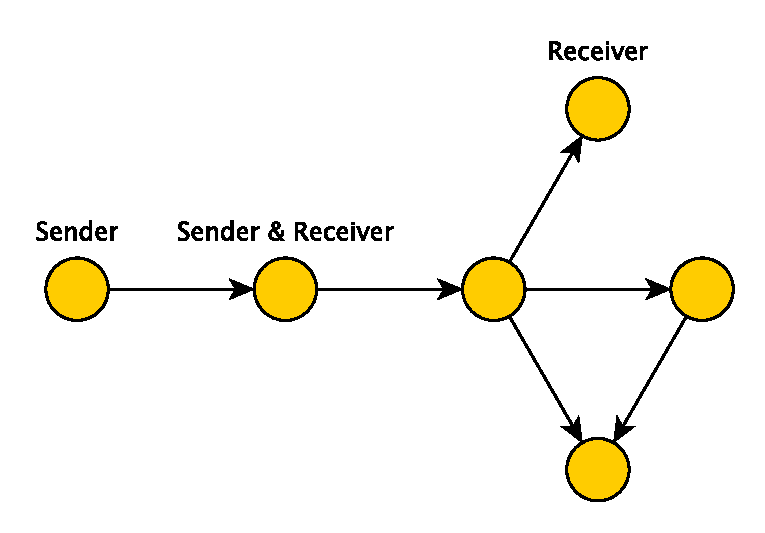
\includegraphics[width=0.48\textwidth]{images/Fig27.pdf}\\
	\caption{Directed graph built on transaction data}
	\label{fig:Fig27}
\end{figure}

Despite the lack of parties' characteristics in the original data, a graph representation is yet powerful, as it provides information about the interaction between parties and reveals the structure of established relationships in the form of a financial network. Having data represented as a graph, it can be exposed to all state-of-the-art network analysis approaches which exploit a network structure. Thus, the financial transaction data with limited information can be extensively studied based on its network structure.
Time is another crucial component of a real-world anonymized financial transaction data which is usually available for analysis. It transforms the underlying network from static to dynamic and allows to cluster users based on both structural and their activity time components.

The opportunity to represent sensitive financial data in a way enabling additional feature retrieval in order to study such data became the motivation for the creation of the current concept.

\section{Idea}
Considering the fact of the high sensibility of financial data and, therefore, its common limited accessibility, the idea of this thesis is splitting financial transaction network participants into segments according to their local structural similarity, global structural similarity and time of activity within the network. 
A number of financial network studies engage traditional Network Analysis approaches to obtain structure-based features including the computation degree, clustering coefficient, PageRank centrality etc. for each node~\cite{ContagionFinNets} ~\cite{StatisticAnalysisFinNetworks}. Although this manual feature engineering provides an insightful outcome in some cases, in others it may be not really helpful or computationally feasible. A method designed in this thesis determines similar participants of a network by their local neighbourhood structures, a global degree attribute, and time attribute. It forms respective segments of nodes making use of an automated feature engineering for networks with semi-supervised algorithms. The method consists of tree main stages: automated feature learning from a network, reducing the dimensionality of the learned continuous space, cluster analysis of nodes' representations in the low-dimension space. 

\subsection{Network feature engineering}
A traditional approach to obtain the structure-based features includes the computation of each network participants' in-degree, out-degree, clustering coefficient, etc. Clustering the nodes based on such features can help in determining segments of similar nodes, but it does not consider the local neighbourhoods of the nodes, which can play an essential role for user segmentation in financial networks and reveal hidden similarities among the participants. Another drawback of the traditional approach is a computation expense. A modern fast alternative to a network feature engineering is network embedding - general method, that aims at learning a low-dimensional latent representation of nodes in a network. Specifically, each node is assigned a dense vector representation based on its local neighbourhood in the feature space and encode community structure as had been shown in ~\cite{chen2018tutorial}. The major advantages over traditional network feature extraction approach are the ability to process large-scale networks in a shorter time, community aware feature learning, producing continuous feature representation space with a number of standard distance metrics and thereby allowing smooth decision boundaries between communities. The network embedding approach is the core of automated feature learning in this master thesis.

Real-world financial networks are constantly evolving, therefore, it is crucial to consider a time component in the network feature learning. However, the majority of the network embedding methods process only static networks, while real-world problems require to preserve both structural information about nodes' neighbourhoods and its operating dynamics. A Node2vec framework developed by Grover and Leskovec ~\cite{node2vec} pioneered alongside some others in the efficient automated feature learning. The analytical usefulness of Node2vec is in building vector representation for a node exploiting the unique flexible neighbourhood sampling strategy, the benefits of which will be discussed in details in \ref{Node2vec}. Originally the framework is intended for static networks. This fact limits its practical application. This master thesis presents a new modification of Node2vec framework which can process a dynamic network and learn features benefiting from its sampling strategy and a time component.

\subsection{Dimensionality reduction}
Dimensionality reduction is the transformation of high-dimensional data into a meaningful representation of reduced dimensionality. Such techniques gained popularity because they help to mitigate undesired properties of high-dimensional space.

The reference linear methods of dimensionality reduction such as PCA or LDA remain ubiquitously used since the last century because of their simplicity and clear interpretability. However, a number of nonlinear dimensionality reduction techniques have been proposed recently in order to better handle real-world data (e.g. t-distributed stochastic neighbor embedding ~\cite{maaten2008visualizing}, uniform manifold approximation and projection ~\cite{mcinnes2018umap}). A concept developed in the current thesis exploits three different linear and nonlinear dimensionality reduction techniques interchangeably. They are described in \ref{Dimensionality Reduction} and used to produce a low-dimensional representation of high-dimensional feature space.

\subsection{Cluster analysis}
The purpose of a cluster analysis is to divide input data into meaningful groups (clusters) so that the objects within a group are similar or related to one another and different from or unrelated to the objects in other groups. Resulting clusters capture the "natural" structure of the data. Clustering is very sensitive to the dimensionality of a processed space. In 1961 Richard Bellman in his book ~\cite{bellman2015adaptive} first identified the term 'curse of dimensionality' referring to the impossibility of optimizing a function of many variables by a brute force search on a discrete multidimensional grid (the number of grid points increases exponentially with dimensionality). Therefore, clustering is applied after the dimensionality reduction step in the frame of the concept in this work. Two clustering techniques - density-based and partitional clustering - are performed interchangeably at the final stage of the concept and described in~\ref{Cluster Analysis}.

\section{Aim and objective}
There is a variety of supervised machine learning methods for Network Analysis based on a set of explicitly given features and/or set of labels. As mentioned above, it is not always possible to have such data or to rely on its authenticity dealing with financial networks. Over recent years, the unsupervised machine learning methods demonstrated their efficiency upon a condition of deficiency of input information. 
One of the bases for feature extraction in unsupervised learning is an item context. For instance, in the case of Semantic Analysis, item context allows to distinguish between the same words having different semantic meaning (Word2vec~\cite{SKIP-GRAM-MODEL}). In case of Network Analysis, a structure of a nearest neighbourhood of a node provides contextual information. 
Though real-world cases in the financial domain are not based on data described by exhaustive feature set, network embedding approach opens up various ways to derive sense out of the raw data that can be represented as a network. Thereby, having no explicit features or data labels, it is still possible to apply network embedding unsupervised learning and derive clusters of nodes which are similar in terms of their neighbourhood structure. It may be highly relevant for the purposes below.
\begin{enumerate}
\item User segmentation based on local neighbourhoods structural similarities and other available graph attributes.
\item Fraud detection based on groups of participant, which are interacted within the similar local neighbourhoods, during the same time period and with roughly the same number of users. Ones one from a group was implicated in fraud, it is worth to pay close attention to other group's participants.
 \end{enumerate}
Unsupervised methods are on high demand for exploring financial transaction data sets since they require minimal number of features such as transfers between a sender and receiver and timestamps of these transfers. This information is usually available the real-world cases.

Various researchers have contributed to the subject by exploring the inherent structure of networks. Lei Tang and Huan Liu in ~\cite{tang2011leveraging} developed a framework for studying heterogeneous social media network based on the network structure. Huang et al in ~\cite{DeepEmbeddingNetworkforClustering} attempted to mine network representations most suitable for cluster analysis and evaluated their approach against the most common cluster techniques and benchmarking data sets. In fact, it is difficult to choose the best network embedding and clustering techniques for segmentation of network participants. Therefore, the developed concept provides a choice among several techniques at each data processing stage. The final results from every possible sequence of techniques are compared to each other. The result with the best score points to the best choice of techniques and their hyperparameters. Only the first stage for the network embeddings learning do not provide a choice of techniques, instead, it allows to choose the relevant graph attributes for learning. 

The majority of existing network embedding methods such as Node2vec~\cite{node2vec}, LINE~\cite{tang2015line}, DeepWalk~\cite{perozzi2014deepwalk} generally exploit a random walk model to learn each node's local neighbourhood. As network nodes are uniquely identified within a network, methods fulfil a homophily hypothesis~\cite{fortunato2010community}: placing embeddings for nodes that are highly interconnected and belong to similar network communities close to each other. An important attribute of real-world networks is time, which describes a network evolution and can contribute a lot to a feature learning. Some dynamic network embedding methods have been recently proposed, e.g. DynamicTriad~\cite{zhou2018dynamic} learns embedding via triadic closure process. The method processes a network by snapshots in every time period and may be slow on large networks.

The overall goal of the work is to present a concept for a users segmentation which reveals new similarities among nodes (users) of a network based on combination of their local neighbourhood structures, time and/or global structural attribute. The contributions of the thesis are:
\begin{itemize}
\item An overview of the state-of-the-art methods for network embedding learning, dimesionality reduction, and clustering.
\item A novel sampling strategy for network embedding, which incorporates local neighbourhoods' structures, time attribute, and global structural attribute (degree) .
\item Implementation of the proposed concept in the form of a multi-staged data science pipeline, which can process any network.
\item The performance evaluation strategy designed for the implemented pipeline
\item Interpretation of the final results produced by the pipeline on a real-world financial data set.
 \end{itemize}
 
\section{Application scenario}
The central concept as well as its implementation in general  can be applied to any kind of networks consisted of nodes connected by edges. The approach itself is domain-independent and does not require any specific adjustment to a subject area. The difference comes in the result interpretation as the revelling patterns are based on user-specific information within a given network.

From mathematical prospective, the concept is able to consume undirected/directed, unweighted/weighted dynamic/static multigraphs with loops. However, in the current work, it will be tested and evaluated on the undirected, unweighted dense multigraph.

A crucial limitation of the concept relates to network density. As the sampling strategy of the feature engineering method uses a random walk on local neighbourhoods of nodes in a network, it implies to process network which nodes are sufficiently connected by edges. In case of a network consists of many disconnected one-node components, a random walk is not able to traverse their local neighbourhoods through adjacent edges and derive representative samples to generate vector representations for such nodes. 

The developed method serves for analysis of real-world networks which are usually characterized by a short average shortest path and a high clustering coefficient comparing to a random network. A network feature learning will not extract any valuable features in case of the initial network structure is uniform across the network. Therefore, the concept is evaluated on a real-world dynamic network.

\section{Summary}
This chapter introduced the thesis, outlined the main idea behind the current work and set up the main motivations and objectives.

The following chapter presents a brief overview of the state-of-the-art approaches used in the present concept. It provides insights into recent literature describing current scientific achievements in the network embedding, dimensionality reduction, and cluster analysis. After that, a reader will find the description of the central concept along with its prototypical implementation details. The rest of the thesis is devoted to results evaluation, interpretation following by a brief summary in conclusion.
\chapter{Background and related work}
\label{cha:background}

This chapter provides an overview of the state-of-the-art approaches for data analysis, which underlay the central concept for user segmentation in financial transaction networks. The major limitations and application restrictions of the methods are discussed here in order to justify future motivations behind the concept in~\ref{cha:conceptanddesign}.

\section{Network Embedding}
Over recent years, network representation learning (NRL) has gained increasing popularity in Network Analysis. NRL or network embedding learning aims to extract features from complex networks and map them into a low-dimensional space. Traditionally, a feature engineering challenge on large networks was solving by tedious manual heuristics such as degree statistics, centrality metrics calculation. However, the recent network embedding approaches can learn feature representations from networks of billions of nodes and edges. Such feature representations come to the more significant result on basic classification and prediction tasks and proved their utility~\cite{node2vec}, ~\cite{perozzi2014deepwalk}, ~\cite{tang2015line}. The ultimate goal of network embedding frameworks is to build a mapping of nodes to a low-dimensional space of features that maximizes a likelihood of preserving network neighbourhoods of nodes.  To learn such mapping, it is necessary to pick an appropriate objective and solve the corresponding optimization problem.  As it will be discussed in~\ref{Skip-gram_Model}, the direct optimization of a downstream prediction task will fail due to the inflatable number of parameters that need to be estimated. The idea of the network-specific objective function came from natural language processing. Tomas Mikolov et al. in~\cite{SKIP-GRAM-MODEL} proposed architecture for computing continuous vector representations of words from very large data sets, which was later adopted by the most well-known frameworks to derive network embeddings.
Generally, the network feature extraction process consists of two main steps: unique sampling procedure which derives subgraphs from the network and skip-gram model for the transformation of the sampled subgraphs into low-dimensional feature vectors. The second step is characteristic for most of the network embedding frameworks. The primary difference is in the sampling strategy.

\subsection{Node2vec}
\label{Node2vec}
Node2vec ~\cite{node2vec} is a framework for the automated semi-supervised scalable feature representation learning in networks. A top-down architecture of Node2vec framework solves a maximum likelihood optimisation problem and learns network embeddings from (un)directed, (un)weighted network. The first step of Node2vec framework is generating sequences of nodes from an input network of arbitrary size according to the specific sampling strategy.

\subsubsection{Sampling strategy}
\label{Sampling strategy}

An appropriate way of network sampling is a critical factor affecting performance and results accuracy of common machine learning tasks in network analysis. Although the idea of NRL has been initially adopted from word representation learning in natural language processing (NLP) domain~\cite{Mikolov:Word2vec}, the sampling strategy for network data could not be inherited from the word sampling strategy within a corpus. Thus, many network embedding frameworks have recently come out competing in the most effective approach for network sampling.
A random walk process is widely used in network embedding methods. Substantially, it is a special case of a Markov chain stochastic model which describes a sequence of possible states with the respective probability depending only on the previous state.
An intuitive heuristic behind the Node2vec sampling lays in understanding properties of the small-world network that the majority of real-world networks demonstrate.
At the very end of the $20^{th}$ century Duncan Watts and Steven Strogatz showed that graphs representing real-world networks usually have a small average shortest path length and a high clustering coefficient in comparison to the Erdős–Rényi random graph where each edge has a fixed probability of being present or absent, independently of the other edges~\cite{watts1998collective}. Therefore, real-world networks demonstrate a tendency of nodes grouping in communities. 
According to Grover and Leskovec, a good sampling strategy strikes a flexible balance between a breadth-first and a depth-first sampling~\cite{node2vec}. A breadth-first sampling considers immediate neighbours of the source and a depth-first sampling aims to sample nodes at increasing distances from the source. Their balance allows to sort out the nodes belonging to the same community closer than the others in the learned low-dimensional space. This is what the Node2vec sample strategy is intended to do. However, the implication of "No free lunch theorem"~\cite{wolpert1997no} is true for a feature learning in networks and there is no optimal sampling strategy that performs best across all networks from different domains and all prediction tasks.

\begin{figure}[H]
	\centering
	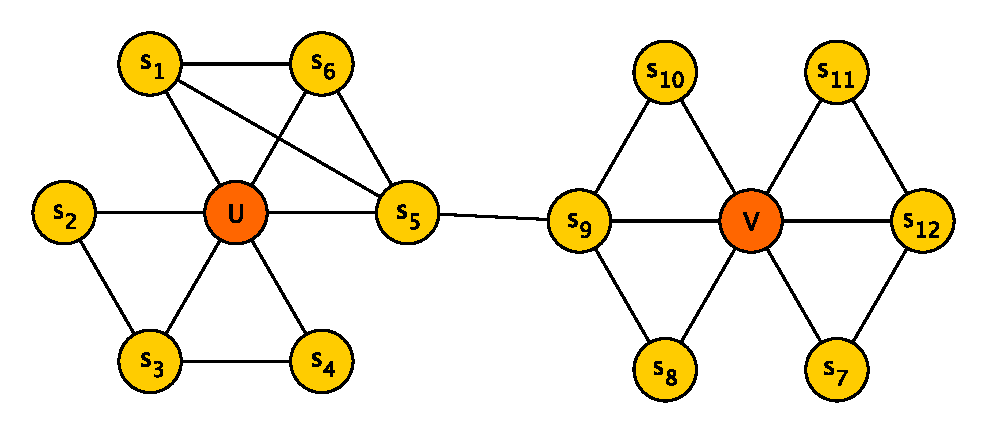
\includegraphics[width=0.5\textwidth]{images/Fig1.pdf}\\
	\caption{Nodes U and V are structurally equivalent; nodes V and s9 belong to the same community}
	\label{fig:Fig1}
\end{figure}

Consider a graph at the~\autoref{fig:Fig1}. A structural equivalence concept states that nodes U and V have the same structural role as a common connection mediating the short path lengths between other nodes. But at the same time, they belong to different communities unlike nodes V and $s_9$, that share the same community - a homophily concept. Due to the structural equivalence hypothesis, nodes U and V should be embedded closely together while nodes V and $s_9$ should be also embedded closely together due to the homophily hypothesis as they belong to the same community.

The unique sampling strategy of Node2vec uses a random walk approach in a graph. It is a stochastic process aimed to describe a path through the successive nodes linked by edges chosen at random. Such technique allows flexible neighbourhoods which can capture at some extent nodes’ structural equivalence along with homophily. The transitions from previous to the next node in a path simulated by random walk process obeys the following distribution law (parameters are explained in the~\autoref{tab:tab1}): 

\begin{equation}
  P(c_i=x | c_{i-1}=v) =
    \begin{cases}
      \frac{\pi_{vx}}{Z} & \text{if $(v,x) \in E$} \\
      0 & \text{otherwise}
    \end{cases}
    \label{eq:equat1}
\end{equation}

\begin{table}
\begin{center}
\begin{tabular}{ | m{1em} | m{2cm}| m{11cm} |} 
\hline
\textbf{\#} & \textbf{parameter} & \textbf{description} \\ 
\hline
1 & $G =(V,E)$ & graph of nodes $V$ and edges $E$ \\ 
\hline
2 & $d_{tx}$ & the shortest path distance between nodes $t$ and $x$ \\
\hline
3 & $l$ & walk length \\
\hline
4 & $u$ & source node \\
\hline
5 & $c_i$ & $i$-th node in the walk \\
\hline
6 & $\pi_{vx}$ & unnormalized transition probability between nodes $v$ and $x$ \\
\hline
7 & $Z$ & normalizing constant \\
\hline
8 & $w_{vx}$ & $vx$ edge weight (=1 for unweighted graphs) \\
\hline
\end{tabular}
\caption {Parameter descriptions}
\label{tab:tab1}
\end{center}
\end {table}

Nove2vec uses a slightly modified~\autoref{eq:equat1} introducing the bias parameter $\alpha$. Assume the random walk process has just transitioned from node $t$ to node $v$ in the~\autoref{fig:Fig2}, the probability to transition from $v$ to any one of its neighbours is $w_{vx} *\alpha$ (normalized), where:

\begin{equation}
  \alpha_{pq}(t,x) = 
    \begin{cases}
      \frac{1}{p} & \text{if $d_{tx}=0$} \\
      1 & \text{if $d_{tx}=1$} \\
      \frac{1}{q} & \text{if $d_{tx}=2$}
    \end{cases}
    \label{eq:equat2}
\end{equation}
\begin{figure}[!hp]
    \vspace{0pt}
    \centering
    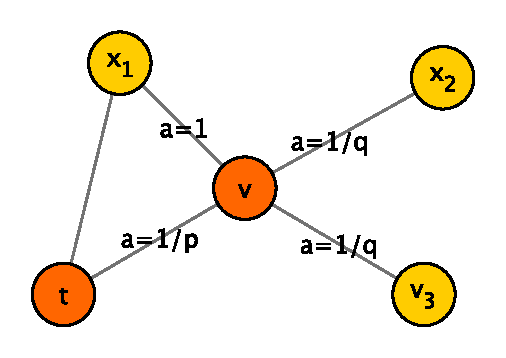
\includegraphics[width=0.4\textwidth]{Fig2.pdf}
    \caption{A random walk process has just traversed edge $(t,v)$. The probabilities of the next transit from $v$ to any node depend on the parameter $\alpha$}
    \label{fig:Fig2}
\end{figure}
As a shortest path $d_{tx} \in \{ 0, 1, 2 \} $ two parameters are sufficient to smoothly control a random walk: $q$ relates to a further neighbourhood exploration (transitions $(v, x_2), (v, x_3)$) and $p$ describes the likelihood of immediately revisiting a node in the walk (transitions $(v, t)$). Together they intuitively control the total speed of random walk in the network exploration in a way described in ~\autoref{tab:tab2}.
\begin{table}[!hp]
\begin{center}
\begin{tabular}{|c|c|c|}
    \hline
    Parameters & Value & Sampling intuitions \\
    \hline
    \multirow{2}{*}{Return parameter $p$} & $> max(q,1)$ & less likely to sample an already-visited node \\\cline{2-3}
    & $< min(q, 1)$ & keep the walk close to the source node \\
    \hline
    \multirow{2}{*}{In-out parameter $q$} & $> 1 $ & bias towards nodes close to source node \\\cline{2-3}
    & $< 1$ & bias towards nodes further away from source node \\
    \hline
\end{tabular}
\end{center}
\caption{Node2vec $p$ and $q$ parameters tuning}
\label{tab:tab2}
\end{table}
Essentially, the conditional transition probability $\pi_{vx}$ of the random walk process, given the present state and one state before, is a function of a preceding node $t$ in the walk ($t -> v -> x$), which makes the random walk a $2^{nd}$ order Markovian. 
The described above sampling algorithm for networks has effective time complexity $O(\frac{l}{k(l-k)})$ per sample~\cite{node2vec}, where a random walk of length $l>k$ can generate k samples for l−k nodes at once. Although a random partial sample reuse across different source nodes can shuttle it insignificantly. It is much better than the classic search-based sampling strategies like breadth-first sampling (BFS) and depth-first sampling (DFS)~\cite{node2vec}. 
The result of the sampling stage of Node2vec framework is a group of directed acyclic graphs generated from the input graph $G(V,E)$. Each of these graphs is a stochastic representation of the node’s neighbourhood. An analogy in NLP would be a text sentence where each word is a node and all words follow a certain order.

\textbf{Limitations. } 
\label{Limitations of Node2vec}
However, the usage of a random walk for sampling exposes some limitations. The set of learned features is unable to transfer to new nodes and graphs as they are tied to vertex identity. Furthermore, the structural hypothesis fails when nodes with similar neighbourhood structures are located within different graph components or sufficiently far from each other. The random walk sampling captures mostly proximity of the nodes in a graph rather than a structural similarity of their neighbourhoods. Goyal and Ferrara demonstrated it in their recent paper ~\cite{Goyal2018GraphET}. This comprehension comes from the fact that nodes are uniquely identified within a graph. Thus, two node embeddings will be placed closer to each other in a low-dimensional space if they have been derived from two overlapping random walk samples, precisely speaking - two samples that have a portion of the same nodes. These flaws and one of the possible solutions have been discussed in 2018 by Nesreen K. Ahmed et al.~\cite{role2vec}. 

\subsubsection{Skip-gram model}
\label{Skip-gram_Model}
At the next stage, the Node2vec framework like some other recent network embedding frameworks ~\cite{perozzi2014deepwalk}, ~\cite{tang2015line} uses a widely known Skip-gram model~\cite{SKIP-GRAM-MODEL} that came from NLP in order to learn continuous feature representations from gathered samples. The model was originally introduced by T. Mikolov et al. in ~\cite{SKIP-GRAM-MODEL} and initially served for learning vector representations of words in a text by optimizing a neighbourhood preserving likelihood objective. Later, it was adapted for feature learning in networks. The core principles of skip-gram model for network embedding will be discussed below.

\textbf{Model objective. }The skip-gram language model is an efficient method for learning high-quality vector representations of words from large amounts of unstructured text data. Specifically, skip-gram maximizes the co-occurrence probability among the words that appear within a window $w$ in a sentence. This intuition came from a hypothesis stated in 1954 by Zellig S. Harris that each language can be described in terms of a distributional structure~\cite{Zellig:DistributionalStructure}. It claims that words in similar contexts tend to have similar meanings, namely words tend to appear in similar contexts.
The~\autoref{fig:Fig3} represents the random walk paths for each node in a graph as a sampling result from \ref{Sampling strategy} where nodes constitute a vocabulary to train the skip-gram model.
\begin{figure}[!hp]
    \centering
    \begin{minipage}{0.45\textwidth}
        \centering
        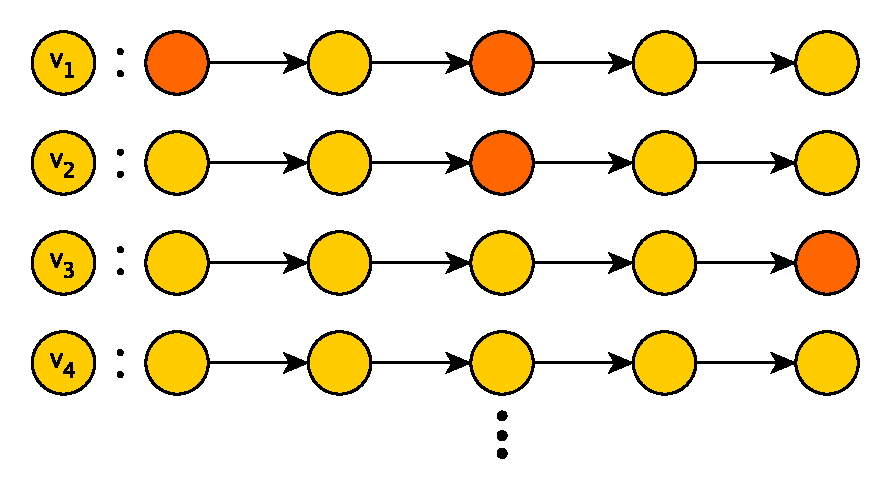
\includegraphics[width=0.9\textwidth]{Fig3.pdf}
        \caption{A group of the directed acyclic graphs sampled from an underlying network}
        \label{fig:Fig3}
    \end{minipage}\hfill
    \begin{minipage}{0.45\textwidth}
        \centering
        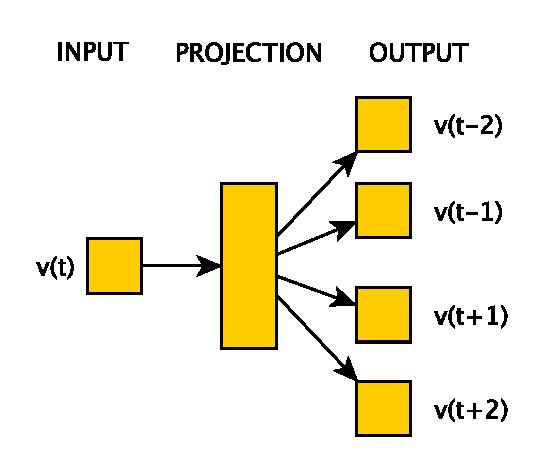
\includegraphics[width=0.9\textwidth]{Fig4.pdf} 
        \caption{Skip-gram model predicts surrounding nodes given the current node}
        \label{fig:Fig4}
    \end{minipage}
\end{figure}
A precise aim of the skip-gram as described in~\cite{SKIP-GRAM-MODEL} is to predict surrounding nodes given a current node. It is achieved by inputting each current node to a log-linear classifier with continuous projection layer, and by predicting nodes within a certain range before and after the current node~\autoref{fig:Fig4}.
Predictions are based on a node proximity to the source node within the sampling graph: more distant nodes get less weight, since they are usually less related to the source node (important: a sampling graph may include a source node more than once in different positions). It is worth to mention that an increasing range of prediction (the length of sample graphs) improves the resulting quality of node representations but at the same time increases computational complexity.
The algorithm estimates continuous representations of nodes by means of recurrent neural network (RNN). The current RNN model architecture was firstly proposed by Tomas Mikolov et al. in 2010 and later described in~\cite{mikolov2013linguistic} in the context of learning continuous word representations. Its adapted version for the network embeddings learning problem is illustrated in~\autoref{fig:Fig5}.

\begin{figure}[H]
    \centering
    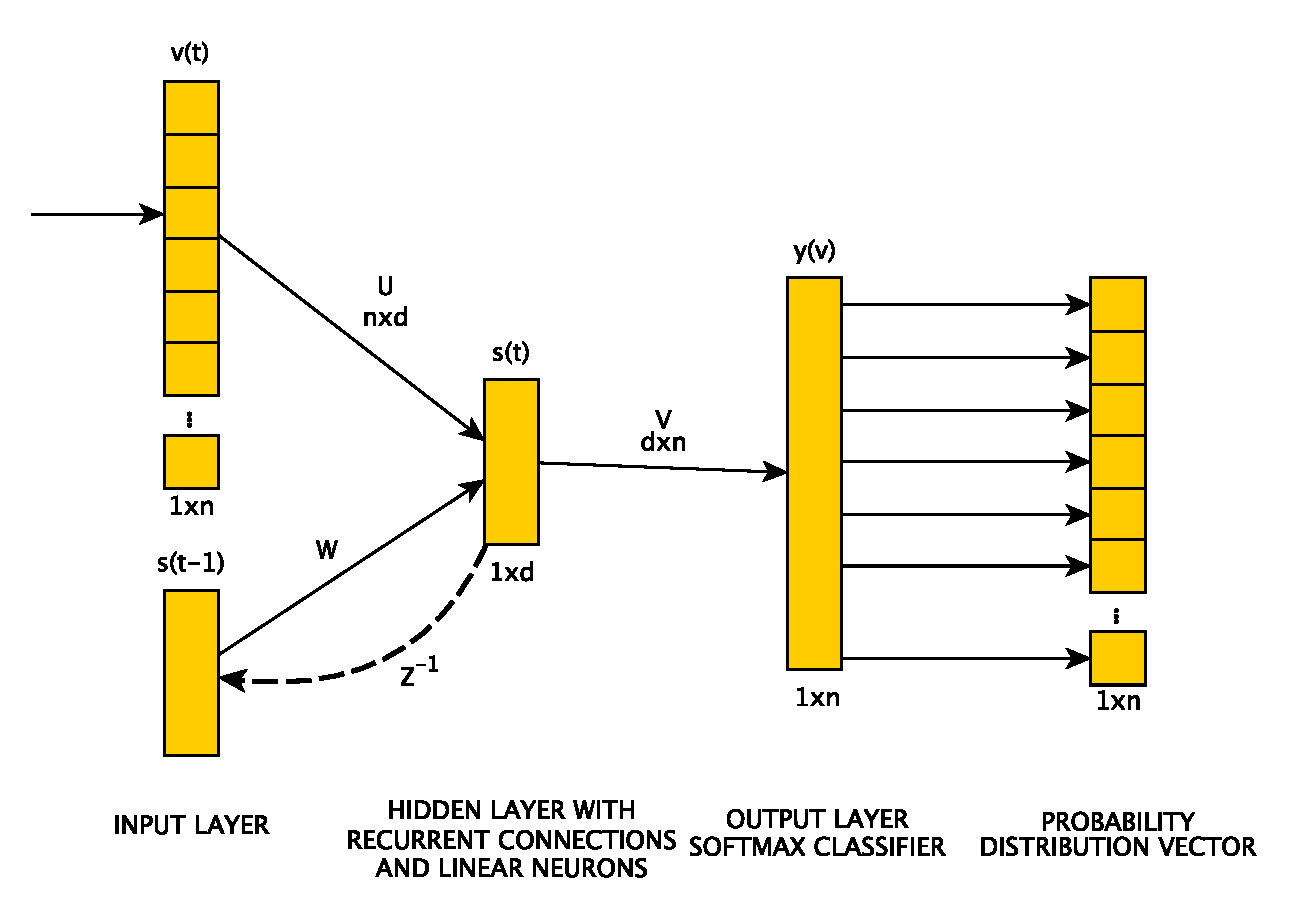
\includegraphics[width=0.7\textwidth]{Fig5.pdf}
    \caption{RNN architecture}
    \label{fig:Fig5}
\end{figure}
\begin{figure}[H]
    \centering
    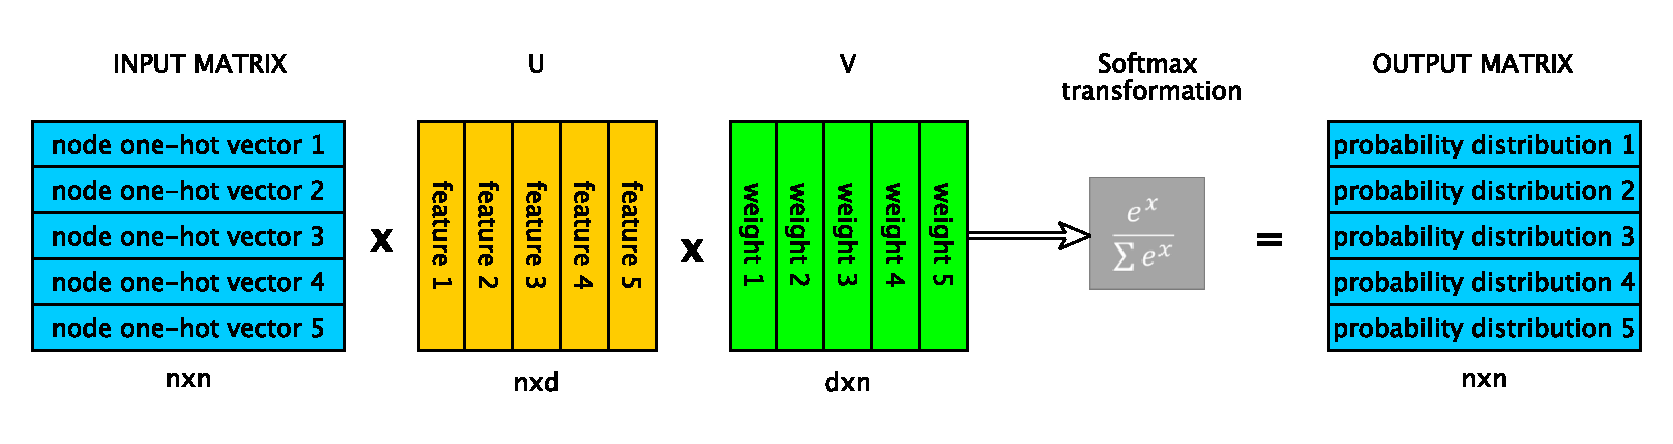
\includegraphics[width=0.7\textwidth]{Fig6.pdf}
    \caption{Probability vectors generation in a matrix notation}
    \label{fig:Fig6}
\end{figure}

Vector $v(t)$ represents an input node at time $t$ encoded using one-hot encoding (vector has “1” in the source node position and “0” in other positions). Vector $v$ has $n$ components, where $n$ is equal to the number of nodes in the underlying network. The output vector $y(v)$ of size $n$ produces a probability distribution over nodes in a network. A hidden layer has $d$ neurons and maps each input vector to its current representation maintaining it over time $t$ by maximizing the probability of source node’s neighbours:
\begin{equation}
  \textbf{s}(t) = f(\textbf{Uw}(t) + \textbf{Ws}(t-1))
    \label{eq:equat3}
\end{equation}
There is no activation function in the hidden layer neurons, and each neuron has a weight vector stored in $\textbf{V}$. Node vectors from the hidden layer $s(t)$ are multiplied with the weight vectors from $\textbf{V}$ and then are subjected to Softmax regression classifier. The last transformation is responsible for each output vector summing up to 1, as they represent some probability distributions. The result from neurons in the output layer is calculated as follows:
\begin{equation}
  \textbf{y}(t) = g(\textbf{Vs}(t)),\;\;\;
  where \;\; f(z)= \frac{1}{1+e^{-z}},\;\;\; g(z_m)=\frac{e^{z_m}}{\sum\limits_{j=1}^n e^{z_j}}
\label{eq:equat4}
\end{equation}
However Softmax classifier at the last step doesn't scale on very large networks. One solution of this problem is "Negative sampling", which will be discussed in \ref{Model training} subsection. ~\autoref{fig:Fig6} illustrates the calculations in a matrix notation. 

Once the RNN is trained via back-propagation, it is not supposed to be used directly for the task it has been trained. Instead, the goal is to learn the hidden layer weight matrix $\textbf{U}$. The columns of the $U$ matrix are the sought-for node representations.

\textbf{Model training. }
\label{Model training}
The described RNN is intended to take a high-dimensional one-hot node vector as an input and output the respective probability distribution as shown in~\autoref{fig:Fig7}.
To train the skip-gram network, one needs to supply it with training example and slightly adjust weights for all neurons in a way that it predicts training sample more accurately. The ultimate prediction task is given a source node to predict the probability for every node in the vocabulary being close to the source. ~\autoref{fig:Fig8} shows how training examples extracted from an underlying network are converted to distribution vectors.

\begin{figure}[H]
    \centering
    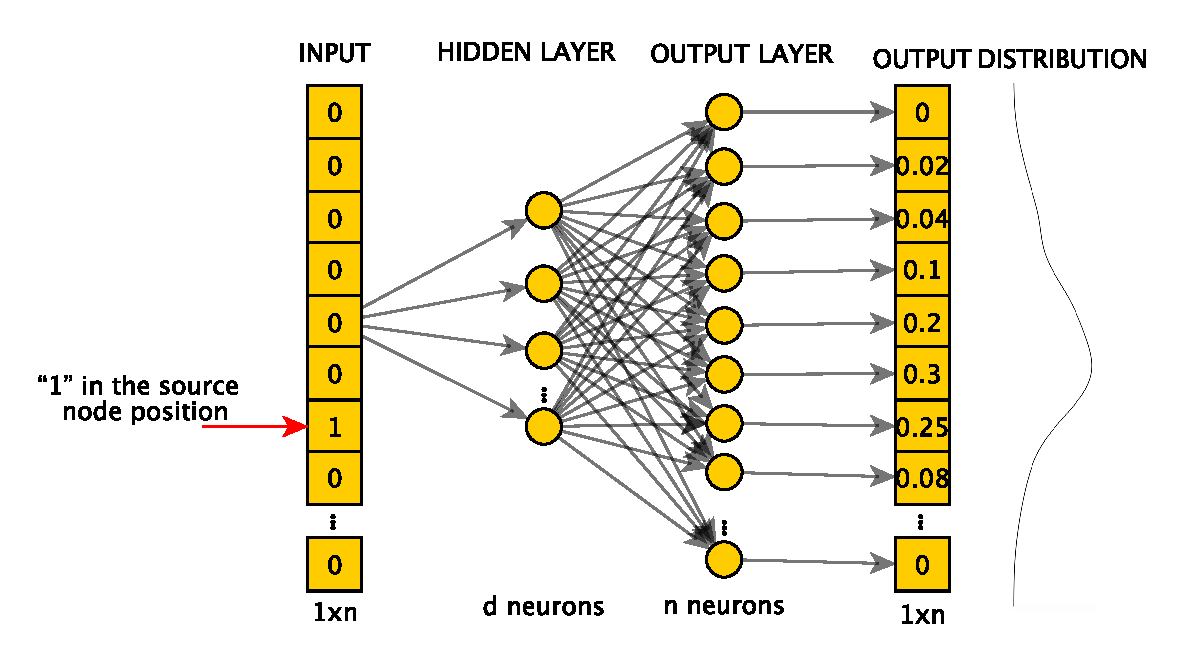
\includegraphics[width=0.7\textwidth]{Fig7.pdf}
    \caption{A group of the directed acyclic graphs sampled from an underlying network}
    \label{fig:Fig7}
\end{figure}
\begin{figure}[H]
    \centering
    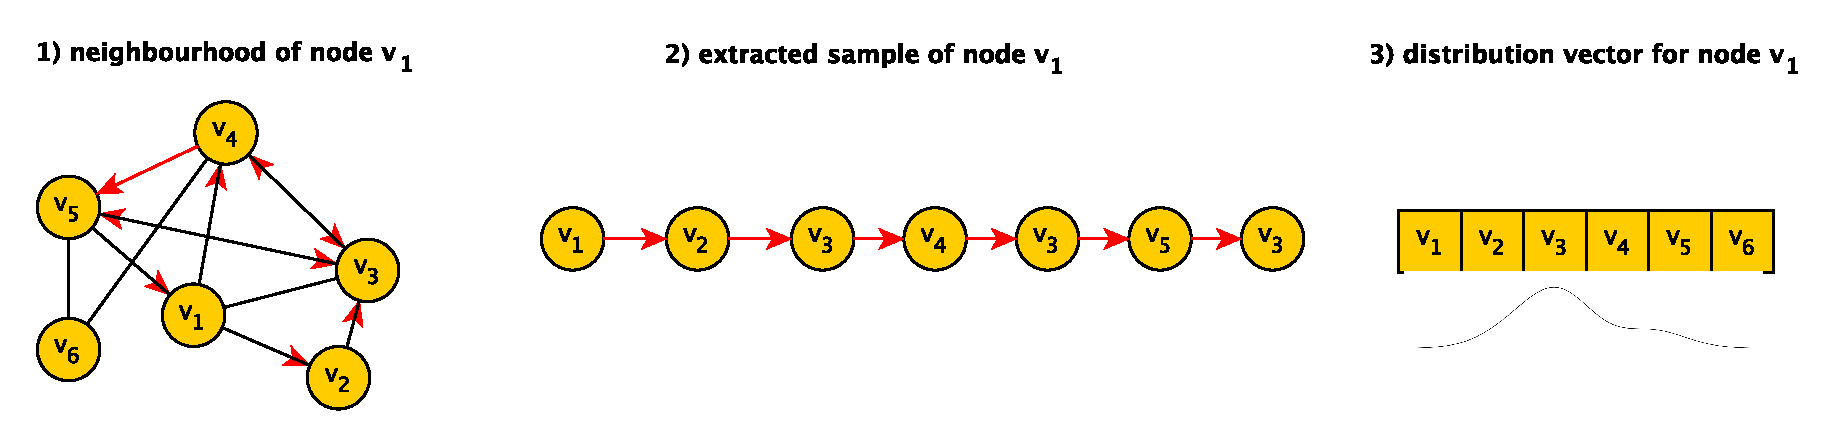
\includegraphics[width=0.7\textwidth]{Fig8.pdf}
    \caption{Skip-gram model predicts surrounding nodes given the current node}
    \label{fig:Fig8}
\end{figure}

Unfortunately, the direct model training for large networks of size $n$ and the number of hidden layer neurons $d$ is in general computationally inefficient as it has to generate $2*n*d$ weights for the hidden and output layers. At the same time, it requires an immense amount of training data to generate all the weights and avoid running into over-fitting. 
To facilitate the training process Mikolov et al. proposed a “Negative sampling” (NEG) in~\cite{gutmann2012noise}. This technique makes the training feasible. The intuition behind is to sample only $k$ negative nodes (negative nodes are those whose one-hot vector has 0 at the source node position) according to some noisy distribution $P_n(v)$ for each source node vector and modify only some weights rather than all of them. Applying NEG the SoftMax objective~\autoref{eq:equat4} transforms into a new one:
\begin{equation}
  \log{f(z_m)} + \sum\limits_{i=1}^k \mathbb{E}_{v_i\sim P_n(v)} [\log{f(z_i)}],\;\; 
  where \;\; f(z)= \frac{1}{1+e^{-z}}
    \label{eq:equat5}
\end{equation}

Running an asynchronous stochastic gradient descend on this modified objective speeds up the training process dramatically what was experimentally shown in~\cite{Mikolov:Word2vec}. Additionally, in this paper Mikolov et al. discussed the choice of $k$ – number of negative samples and $P_n(v)$ – node-specific distribution. In general, for large networks $k$ is supposed fluctuating from 2 to 5 negative node-vectors, drawn from $P_n(v)$ - a unigram term frequency distribution.

\begin{figure}[H]
    \centering
    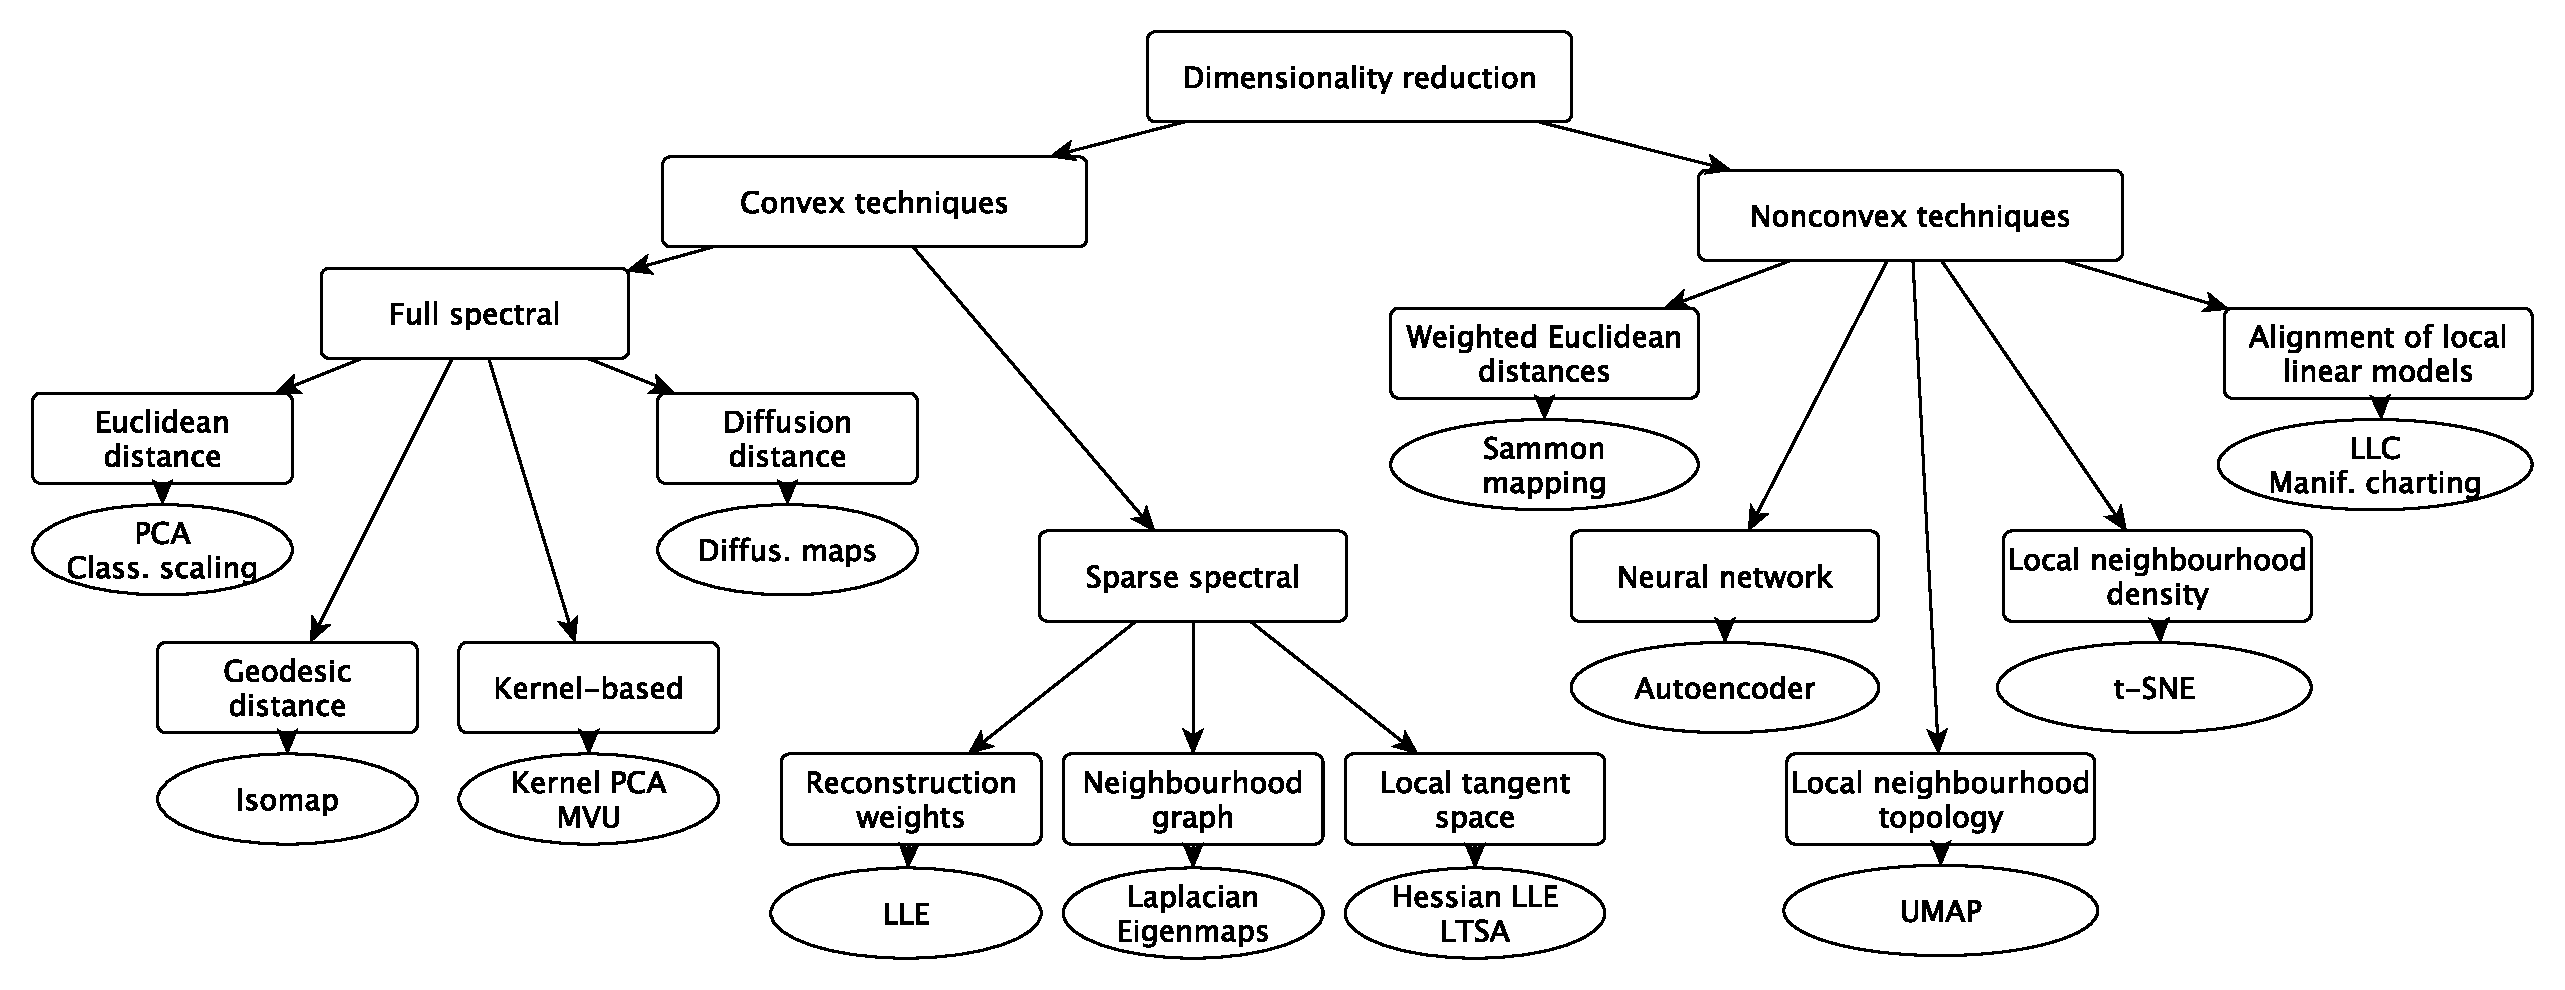
\includegraphics[width=1.0\textwidth]{Fig10.pdf}
    \caption{Taxonomy of dimensionality reduction techniques}
    \label{fig:Fig10}
\end{figure}

\section{Dimensionality Reduction}
\label{Dimensionality Reduction}
Dimensionality reduction is the transformation of high-dimensional data into a meaningful representation of reduced dimensionality. In the ideal case, a reduced representation should have a dimensionality equal to the data intrinsic dimensionality what means a minimum number of parameters needed to account for observed properties of the data. Dimensionality reduction is important to this work as it mitigates the "curse of dimensionality" which naturally occurs in high-dimensional feature space learned from a network at the previous pipeline stage.

~\autoref{fig:Fig10} exhibits an extended taxonomy of techniques for dimensionality reduction inspired by~\cite{van2009dimensionality}. The upper subdivision into convex and non-convex techniques comes from the objective function that has to be optimized. A convex techniques' objective function does not contain a local optima in the convex solution space and can be optimized by solving a generalized eigenproblem. The further subdivision of convex techniques is based on the performance of an eigendecomposition of a full matrix or a sparse matrix. An objective functions of non-convex techniques do contain local optima. The extensive overview of all techniques mentioned in the taxonomy could be found in ~\cite{van2009dimensionality}.

\subsection{Principal Components Analysis}
Although in the last decades many nonlinear dimensionality reduction techniques have been proposed, the linear PCA remains the most popular unsupervised method because of its simplicity and solid result interpretability. It transforms linearly the original input which is typically high-dimensional into new uncorrelated features. The ultimate goal is to find a low-dimensional representation of the data preserving as much of the variance in the input data as possible. The PCA became of great demand in machine learning as it cleans up the data from extraneous variables which in fact contain little information. Thus, it allows to speed up perceptibly machine learning algorithms performance at the cost of accuracy. Finally, another major application scenario of PCA is data visualization. It allows approximate visualization high-dimensional data in 1D, 2D or 3D space by taking the axes along the directions of the highest variances in the data. The concept consists of several steps, which will be described below.

\textbf{Concept. }
The first step of PCA is a standardization of the input data, what means to subtract from each feature its mean and divide by its standard deviation. The second step is to obtain the basis of orthogonal eigenvectors and spectrum from the covariance matrix of standardized data. The next is sorting the calculated eigenvalues in descending order and consider the first $k < n$ where $k$ is a desired number of dimensions and $n$ is dimensionality of the original space. After, construct the projection matrix from the eigenvectors that correspond to the chosen ordered $k$ eigenvalues. Finally, to obtain the new representation of the data in the reduced $k$-dimensional space transform the original data set by multiplying it by the projection matrix.
In mathematical terms, PCA solves the standard eigenproblem for covariance matrix in case of standardized data~\autoref{eq:equat6} (for correlation matrix in case of non-standardized data).

\begin{equation}
  cov(\textbf{X})\textbf{M} = \lambda \textbf{M}
    \label{eq:equat6}
\end{equation}

where $cov(\textbf{X})$ is the sample covariance matrix of the standardized data $\textbf{X}$ and $\textbf{M}$ is the linear basis of eigenvectors. The trick allows to reduce the output space in matrix $\textbf{M}$, that consists of the $k$ eigenvectors corresponded to the largest eigenvalues of the $cov(\textbf{X})$. Thus, the sought-for low-dimensional data representation is 

\begin{equation}
  \textbf{Y} = \textbf{X}\textbf{M}
    \label{eq:equat7}
\end{equation}

\textbf{Limitations. }The fact that nowadays the linear PCA remains at the peak of popularity among dimensionality reduction techniques in machine learning after more than a century from its first formulation by Karl Pearson proves its ubiquitous practical value. Nevertheless, a comparative review of dimensionality reduction techniques from 2009 ~\cite{van2009dimensionality} shows that nonlinear techniques outperform linear techniques on selected data sets that typically contain well-sampled smooth manifolds. But that does not guarantee anything regarding the real-world data. In fact, they show that most nonlinear techniques do not outperform linear PCA on natural data sets. 
In general, full spectral linear dimensionality reduction techniques like PCA suffer from the inability of modelling complex nonlinear manifolds. This idea has been clearly illustrated by Laurens van der Maaten in ~\cite{maaten2008visualizing} on a toy example - a “Swiss roll” data set ~\autoref{fig:Fig11}. This necessitates a search for other intuitions unlike preserving large pairwise distances to maximize variance like PCA does. Another drawback concerns the information loss: a new representation of the data will no longer contain the information from those features that have been excluded.

\begin{figure}[H]
    \centering
    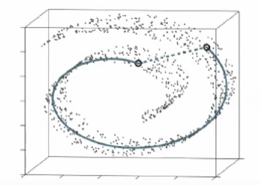
\includegraphics[width=0.5\textwidth]{Fig11.png}
    \caption{A Swiss Roll data set plotted in 3D space. PCA will fail to find non-linear circular path. Data source: http://people.cs.uchicago.edu/~dinoj/manifold/swissroll.html}
    \label{fig:Fig11}
\end{figure}

\subsection{t-Distributed Stochastic Neighbour Embedding}
t-Distributed Stochastic Neighbour Embedding is an unsupervised nonlinear dimensionality reduction technique that aims to preserve the local structure of data in a visualization task. It has been initially proposed by Laurens van der Maaten and Geoffrey Hinton in~\cite{maaten2008visualizing} as an optimisation of stochastic neighbour embedding ~\cite{hinton2003stochastic} to overcome its main flaw - an excessive crowding of objects while mapping them to low-dimensional space. L. van der Maaten and G. Hinton compared in their study seven most known nonlinear techniques against t-SNE and revealed that t-SNE outperforms others in visualisation of a MNIST data set \footnote{The MNIST data set contains 60,000 grayscale training images of handwritten digits and is publicly available from http://yann.lecun.com/exdb/mnist/index.html} and separates objects of different digits better than other techniques.
The t-SNE concept on a high level looks as follows: the algorithm calculates two similarity measures between pairs of instances in a high dimensional space and in low dimensional space and tries to optimize them using a cost function.

\textbf{Concept. }~\autoref{fig:Fig12} shows some points in a high dimensional space. To measure similarities between these points, t-SNE centres a Gaussian over a point $x_i$ and consider its local neighbourhood. Instead of calculating all pairwise distances between points like full spectral techniques do, t-SNE measures only local distances to nearby points. A conditional probability density function $p$ describes the probability of two points being close to each other and is constructed as follows:

\begin{equation}
  p_{j|i}=\frac{\exp{(-||x_i-x_j||^2/2\sigma_{i}^2)}}{\sum_{j`\neq i}\exp{(-||x_i-x_j`||^2/2\sigma_{i}^2)}}
    \label{eq:equat8}
\end{equation}

\begin{figure}[H]
    \centering
    \begin{minipage}{0.45\textwidth}
        \centering
        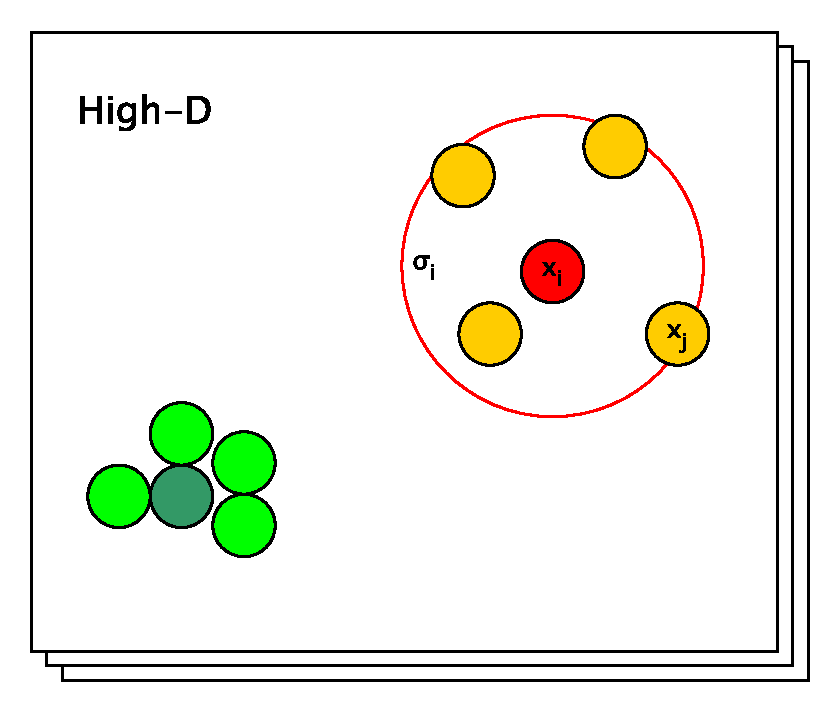
\includegraphics[width=0.9\textwidth]{Fig12.pdf}
        \caption{Points in a high dimensional space are not equally distributed. Perplexity parameter of t-SNE is responsible to scale bandwidth $\sigma_i$ to consider a roughly fixed number of points within each Gaussian.}
        \label{fig:Fig12}
    \end{minipage}\hfill
    \begin{minipage}{0.45\textwidth}
        \centering
        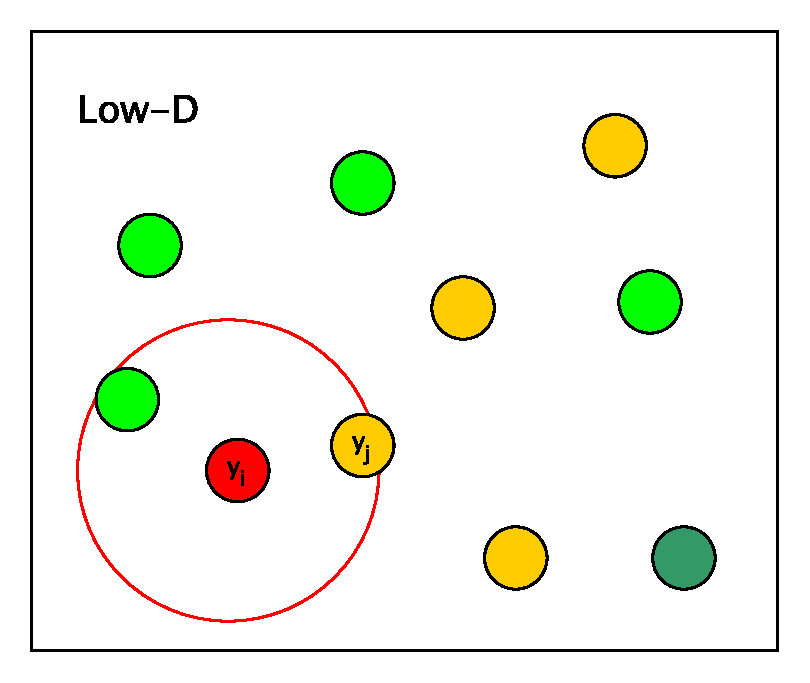
\includegraphics[width=0.9\textwidth]{Fig13.pdf} 
        \caption{Initial representations of points from a high-D space in a low-D space. The discrepancies between pairwise distances in a high-D and low-D are optimized by the gradient of the objective function.}
        \label{fig:Fig13}
    \end{minipage}
\end{figure}

$x_i$ is the fixed centre of the Gaussian and $x_j$ are other points under this gaussian. The bottom part of the equation is a normalization factor specific to this particular Gaussian that normalizes probabilities over pairs that involves point $x_i$. This way of normalization allows to set a different bandwidth of $\sigma_i$ for each point and thereby fix perplexity for the conditional distribution. ~\autoref{fig:Fig12} demonstrates the scaling of the bandwidths of the Gaussians depending on the number of points falls into the Gaussians. Points in the original space are typically distributed nonuniformly and this scaling technique enables to adapt to different densities.
The further assumption is the final joint probability $p_{ij}$ is a summarized average of the conditional probabilities $p_{j|i}$ and $p_{i|j}$:

\begin{equation}
  p_{ij}=\frac{p_{j|i} + p_{i|j}}{2N}
    \label{eq:equat9}
\end{equation}

In fact, the probability $p_{ij}$ is proportional to the similarity of points $x_i$ and $x_j$. A large magnitude for $p_{ij}$ signalizes two points $x_i$ and $x_j$ are close together in the original high-dimensional space and infinitely small $p_{ij}$ implies two points are far apart.
The next step is to build low-dimensional representations for each point from the high-dimensional space. Assume these representations are on the ~\autoref{fig:Fig13}. To come up with the similar probabilistic measure of points similarities, construct a function with a kernel distribution centered in $y_i$:

\begin{equation}
  q_{ij}=\frac{(1+||y_i-y_j||^2)^{-1}}{\sum_{k}\sum_{l\neq k}(1+||y_k-y_l||^2)^{-1}}
    \label{eq:equat10}
\end{equation}

the bottom part here is a normalization factor over all pairs of points in the low-D space. The probability $q_{ij}$ measures the similarity of $y_i$ and $y_j$. 
The ultimate goal of the algorithm is to minimize the difference between two probability functions $p$ and $q$ in a way that $q$ is a reflection of the ground truth $p$. A common measure of entropy - Kullback–Leibler divergence is used for this purpose:

The KL criterion is a "distance measure" of two probability distributions that is necessary to be minimized over all pairs of points via gradient descent for the current task. The asymmetry of the KL divergence facilitates to preserve local structure of points in the high-D space. Assume that $x_i$ and $x_j$ are close together and thus $p_{ij}$ value is large. In order to minimize the sum of the KL divergences in the ~\autoref{eq:equat11} the $q_{ij}$ has to be also a large value. That means that the corresponding points $y_i$ and $y_j$ in the low-D are also close together. Overall, the optimizing procedure of the KL divergences tries to model large values of $p_{ij}$ by corresponding large values of $q_{ij}$. Although, because of the asymmetry of the KL divergence, it does not guarantee the same for the inverse case: if two points are very dissimilar (small $p_{ij}$), then the corresponding contribution to the sum is very small and by this irrelevant regardless of a $q_{ij}$ value. This fact enables t-SNE to capture local structures of a high-D space.

One of the crucial enhancements over the antecedent Stochastic neighbour embedding approach (SNE) ~\cite{hinton2003stochastic} is a usage of Student t-distribution with one degree of freedom instead of normal for $q$ in the ~\autoref{eq:equat10}. ~\autoref{fig:Fig14} demonstrates the clear difference in the shapes of two distributions. Student t-distribution is a lot more heavy-tailed compared to a Gaussian. Assume the probability $q_{ij}$ is low and points $y_i$ and $y_j$ are dissimilar. Because of using a heavy-tailed distribution the points will be placed too far apart from each other and thereby will not crowd around the centre. The crowding problem of SNE under the Gaussian distribution has been clearly described in ~\cite{maaten2008visualizing}.

\begin{equation}
  C = \sum_{i}KL(P_i||Q_i)=\sum_{i}\sum_{i\neq j}p_{ij}\log{\frac{p_{ij}}{q_{ij}}}
    \label{eq:equat11}
\end{equation}

\begin{figure}[!hp]
    \centering
    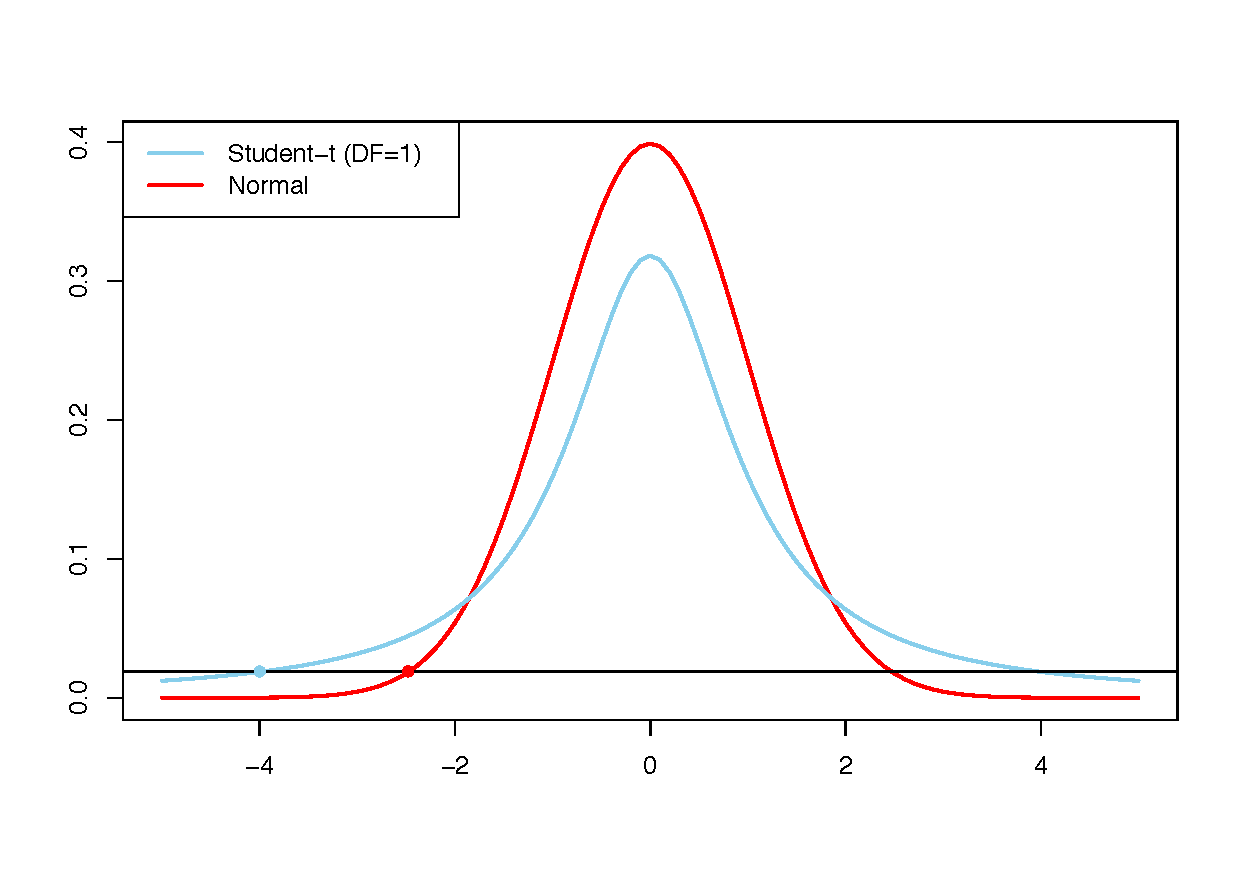
\includegraphics[width=0.5\textwidth]{Fig14.pdf}
    \caption{Heavy-tailed distribution allows two dissimilar points to be far apart from each other in the projected low-D space, as on the same low value of probability (referencing dissimilar points), the Student t-distribution places two points further apart.}
    \label{fig:Fig14}
\end{figure}

\textbf{Model objective and optimization. }
As mentioned above the cost function of t-SNE is a sum of Kullback–Leibler divergences which optimized by gradient descent. The gradient of the KL divergence between the Gaussian distribution $P$ and the Student t-distribution $Q$ with respect to a point is given by:

\begin{equation}
  \frac{\partial C}{\partial y_i}= 4\sum_{j\neq i}\underbrace{(p_{ij}-q_{ij})(1+||y_i-y_j||^2)^{-1}}_\text{I}\underbrace{(y_i-y_j)}_\text{II}
    \label{eq:equat12}
\end{equation}

The transformation of ~\autoref{eq:equat12} into ~\autoref{eq:equat11} is covered in Appendix A of ~\cite{maaten2008visualizing}. The second part of the gradient (II) is a directed spring between pair of nodes and the first part (I) measures an exertion of this spring based on the difference between $p_{ij}$ and $q_{ij}$. This difference is equal to zero if $q_{ij}$ models $p_{ij}$ perfectly. The optimization process is moving points around the fixed one at each step until to attain a lower KL divergence.
A computation of t-SNE representations outperform SNE as a Student t-distribution does not involve an exponential unlike a Gaussian and thereby density evaluation of a point is faster.

\textbf{Limitations. }
As gradient of the model objective considers all pairwise interactions between points, having $n$ points the $n^2$ interactions between them have to be considered and sum in every gradient update. This limits a t-SNE application to 5 000 - 10 000 points in a space. This restriction could be mitigated applying Barnes-Hut approximation ~\cite{Barnes1986}: instead of calculating every pairwise distance, group points together where possible to calculate one distance between point and group of points.
Another major weakness of t-SNE is in its nonconvex cost function. An output solution is stochastic and depend on optimization parameters. It may vary each t-SNE run even preserving the same set of optimization parameters, however, the quality of the optima does not change much from run to run.
t-SNE fails to preserve pairwise distances on a global structural level. On the  ~\autoref{fig:Fig15} two Gaussians with scaling bandwidths $\sigma_i$ and $\sigma_j$ are centered at $x_i$ and $x_j$. The respective conditional probabilities are evidently $p_{j|i} > p_{i|j}$ under a perplexity optimization parameter. The final joint probability $p_{ij}$ is the average of conditionals for two points viewed within their local neighbourhoods. Thereby the resulting probability $p_{ij}$ may not reflect the true pairwise distance on a global structural view and points' counterparts in the low-D will not globally preserve relevant distances. It follows that, in general, t-SNE does not preserve either distances nor density of the original space, it aims to reflect the structures observed in the high-D space by learning local neighbourhoods of points. 

\begin{figure}[!hp]
    \centering
    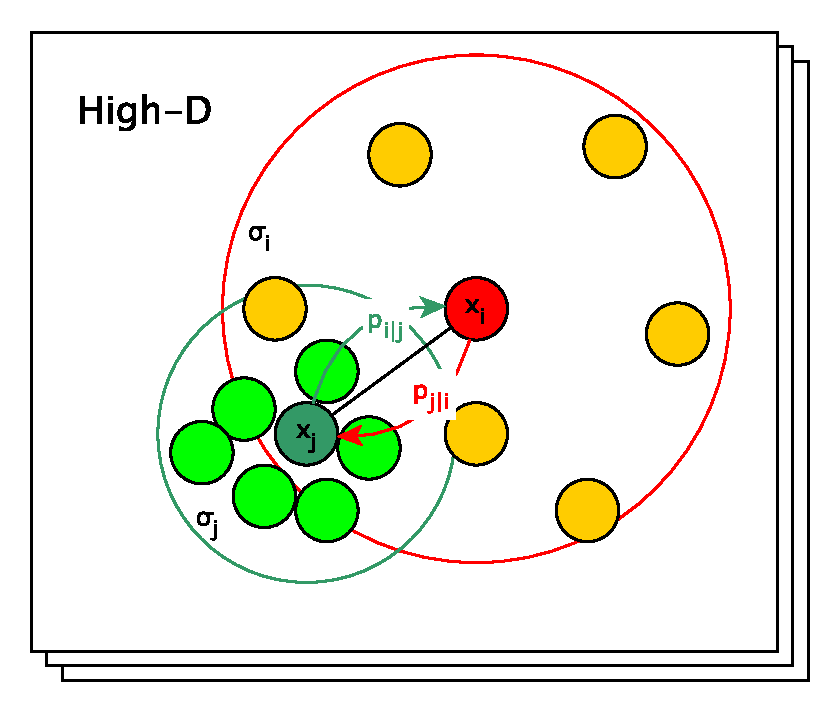
\includegraphics[width=0.5\textwidth]{Fig15.pdf}
    \caption{Example of the points distribution in a high-dimensional space when t-SNE mapping fails to preserve pairwise distance.}
    \label{fig:Fig15}
\end{figure}

t-SNE does not guarantee to reflect the same density clusters present in the original space, therefore density based algorithms should be applied on a t-SNE output with forethought, caution, and understanding the consequences or replaced by other techniques. Authors promote the technique as being well suited for data exploration and visualizing high-dimensional data, however conducting cluster analysis on t-SNE output is quite common in practice.

\subsection{Uniform Manifold Approximation and Projection}
One of the most recent technique from 2018 for dimensionality reduction is Uniform Manifold Approximation and Projection (UMAP). It is a competitor of t-SNE for visualization quality, and according to its creators, it preserves more of the global structure of the original data ~\cite{mcinnes2018umap}. Unlike t-SNE, UMAP has been presented as a dimension reduction technique for machine learning of general purpose.
Umap operates on Riemannian Manifolds and is able to recognize dense structures of arbitrary shape. It is faster than t-SNE, can handle larger high dimensional data sets, is able to scale well and better preserves a global structure of the data. 
The general idea behind UMAP is similar to t-SNE: construct two topological representations from the original high dimensional data and from some low dimensional representation and minimize the cross-entropy between the two topological representations. 

Assume some topological spaces constricted out of simple combinatorial components - simplices\footnote{\textbf{Simplex} - a generalization of the notion of a triangle or tetrahedron to arbitrary dimensions. Source: www.wikipedia.org}. A k-dimensional simplex (k-simplex) is formed by covering $k+1$ independent points by convex hull. On ~\autoref{fig:Fig17} each k+1-simplex consists of several k-simplices. This structural nesting allows generalization of topological spaces to arbitrary dimensions.

\begin{figure}[!hp]
    \centering
    \begin{minipage}{0.45\textwidth}
        \centering
        
\includegraphics[width=1.2\textwidth]{Fig17.png}
        \caption{Low dimensional simplices.}
        \label{fig:Fig17}
    \end{minipage}\hfill
    \begin{minipage}{0.45\textwidth}
        \centering
        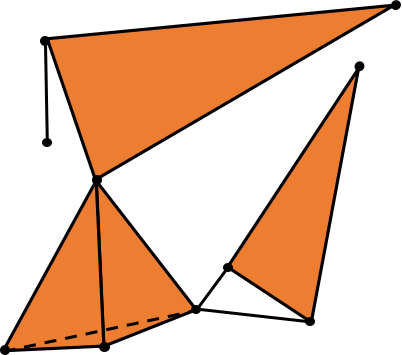
\includegraphics[width=0.45\textwidth]{Fig16_1.png} 
        \caption{Three-dimensional simplicial complex.}
        \label{fig:Fig16}
    \end{minipage}
\end{figure}

A simplicial complex on ~\autoref{fig:Fig16} is glueing together k-simplices along their faces (a dot is a face of 0-simplex, an edge is a face of 2 q-simplex, etc.). It serves for constructing topological spaces out of simplices of various dimensions~\cite{gamelin1999introduction}.
The goal is to cover finite sets of data points from Euclidean topology in a high-dimensional space by a simplicial complex. For this purpose, one can use open cover\footnote{\textbf{Open cover} - a collection of open sets of a topological space which union contains a given subset. For example, an open cover of the real line, with respect to the Euclidean topology, is a set of all open intervals (-n,n), where n in N. Source: http://mathworld.wolfram.com} to cover all sets in space. A Čech complex~\cite{MR1867354} provides a combinatorial way to convert open cover into a simplicial complex in the following simplified way: assume each set in the cover to be a 0-simplex, a 1-simplex is built between two such intersected sets, a 2-simplex spans three of such sets if their triple intersection is non-empty, etc. A solid mathematical justification of this process producing the meaningful topological space firstly has been formulated by K.Borsuk in 1948~\cite{Borsuk1948}, reviewed and proved later in many sources including ~\cite{MR1867354}, and nowadays is referenced as the Nerve theorem.
To learn about the topology of original space, one generates an open cover of it. To approximate an open cover, one can cover each point from the original finite set in a metric space with spheres of radius r. The process of learning a simplicial complex from the metric space is formally depicted on ~\autoref{fig:Fig18}.

\begin{figure}[!hp]
    \centering
    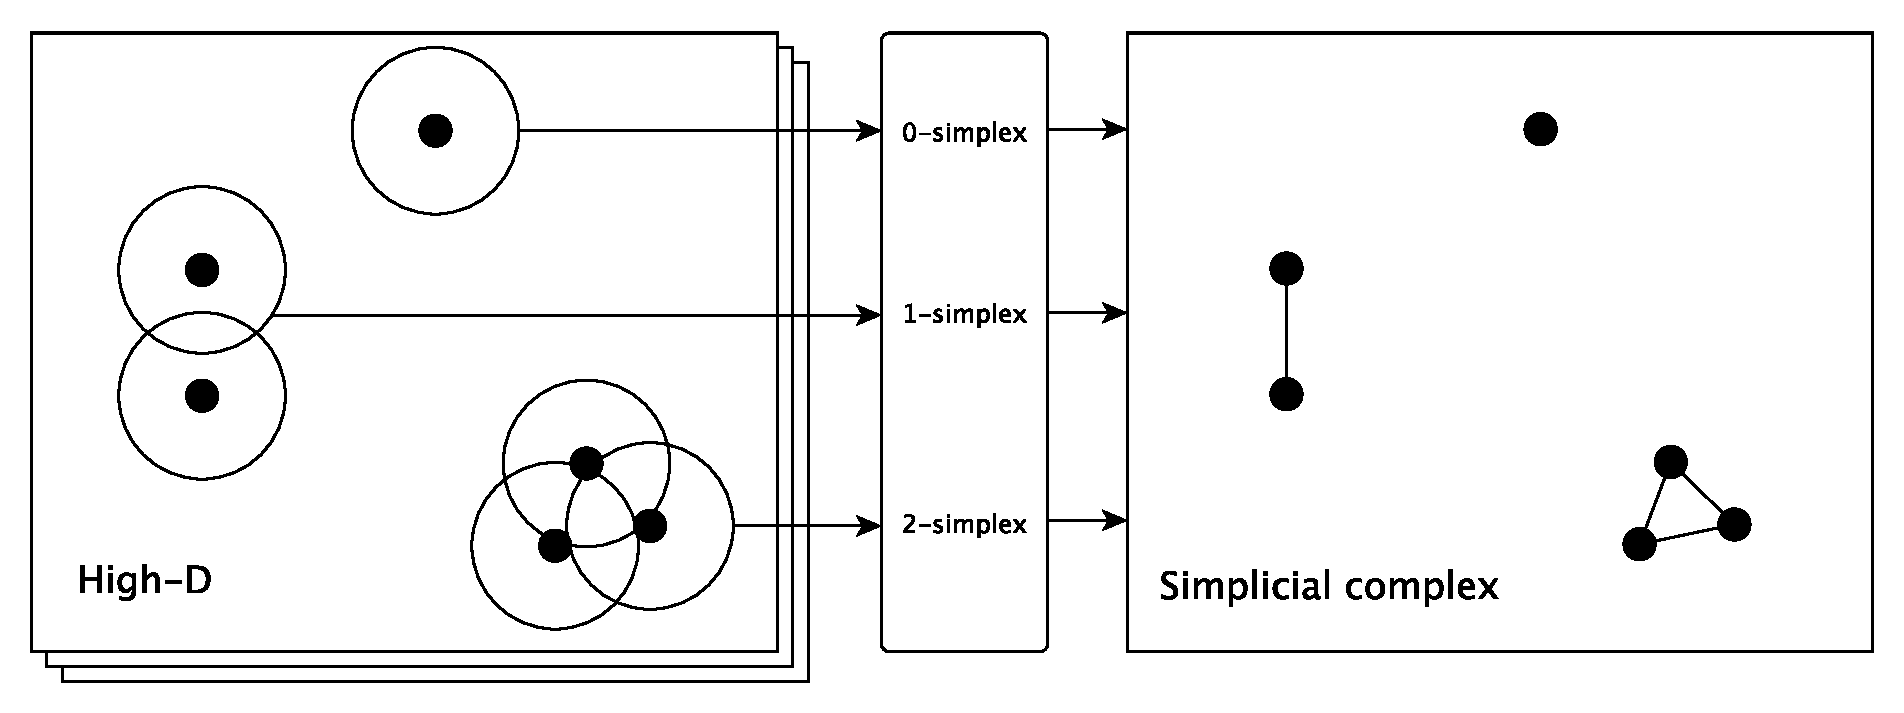
\includegraphics[width=0.8\textwidth]{Fig18.pdf}
    \caption{Process of learning a simplicial complex.}
    \label{fig:Fig18}
\end{figure}

Authors of the UMAP paper~\cite{mcinnes2018umap} proved that a simplicial complex indeed captures the fundamental topology better other approaches used by competitors like t-SNE. From the topological representation one can farther build a low dimensional representation for the data of similar topological representation. 
One of the toughest practical challenges is to come up with the right radius r of the spheres in an open cover approximation process~\autoref{fig:Fig18}. The precise math-justified way of choosing the proper radius corresponding to the distance function defined unequally for each point of the original space is expounded in ~\cite{mcinnes2018umap} and basically follows the assumption that the points are uniformly distributed in a warping space with a certain distribution of distances.

\textbf{Model objective and optimization. }
By analogy with t-SNE, the next intuition is to find a low dimensional representation with as similar topological structure as possible. To attain it, one has to define an objective that aims to minimize the difference between two topological structure. The comparing topological structures shares the same 0-simplices (same points). Consider them as two vectors of probabilities indexed by the 1-simplices, where the simplex either exists or doesn’t. Under this perspective, the cost function is the cross entropy between two Bernoulli variables and is defined as follows:

\begin{equation}
  C = \sum_{e\in E} \underbrace{w_h(e)\log \frac{w_h(e)}{w_l(e)}}_\text{I} + \underbrace{(1-w_h(e))\log \frac{1-w_h(e)}{1-w_l(e)}}_\text{II}
  \label{eq:equat13}
\end{equation}

where $E$ is a set of all possible 1-simplices, $w_h(e)$ is the weight of the 1-simplex $e$ in the high-dimensional space, $w_l(e)$ is the weight of the 1-simplex $e$ in the low-dimensional representation. The first part I of the~\autoref{eq:equat13} characterizes an attractive force between the points of $e$ and the second part II - a repulsive force between them. The stochastic gradient descent optimization process applied to this cost function moves around points in a low-dimensional space affect $w_h(e)$ and $w_l(e)$ in a way finally allow the topological structure of the low-dimensional space reflect relatively accurately the overall topology of the source data.

\begin{figure}[H]
    \centering
    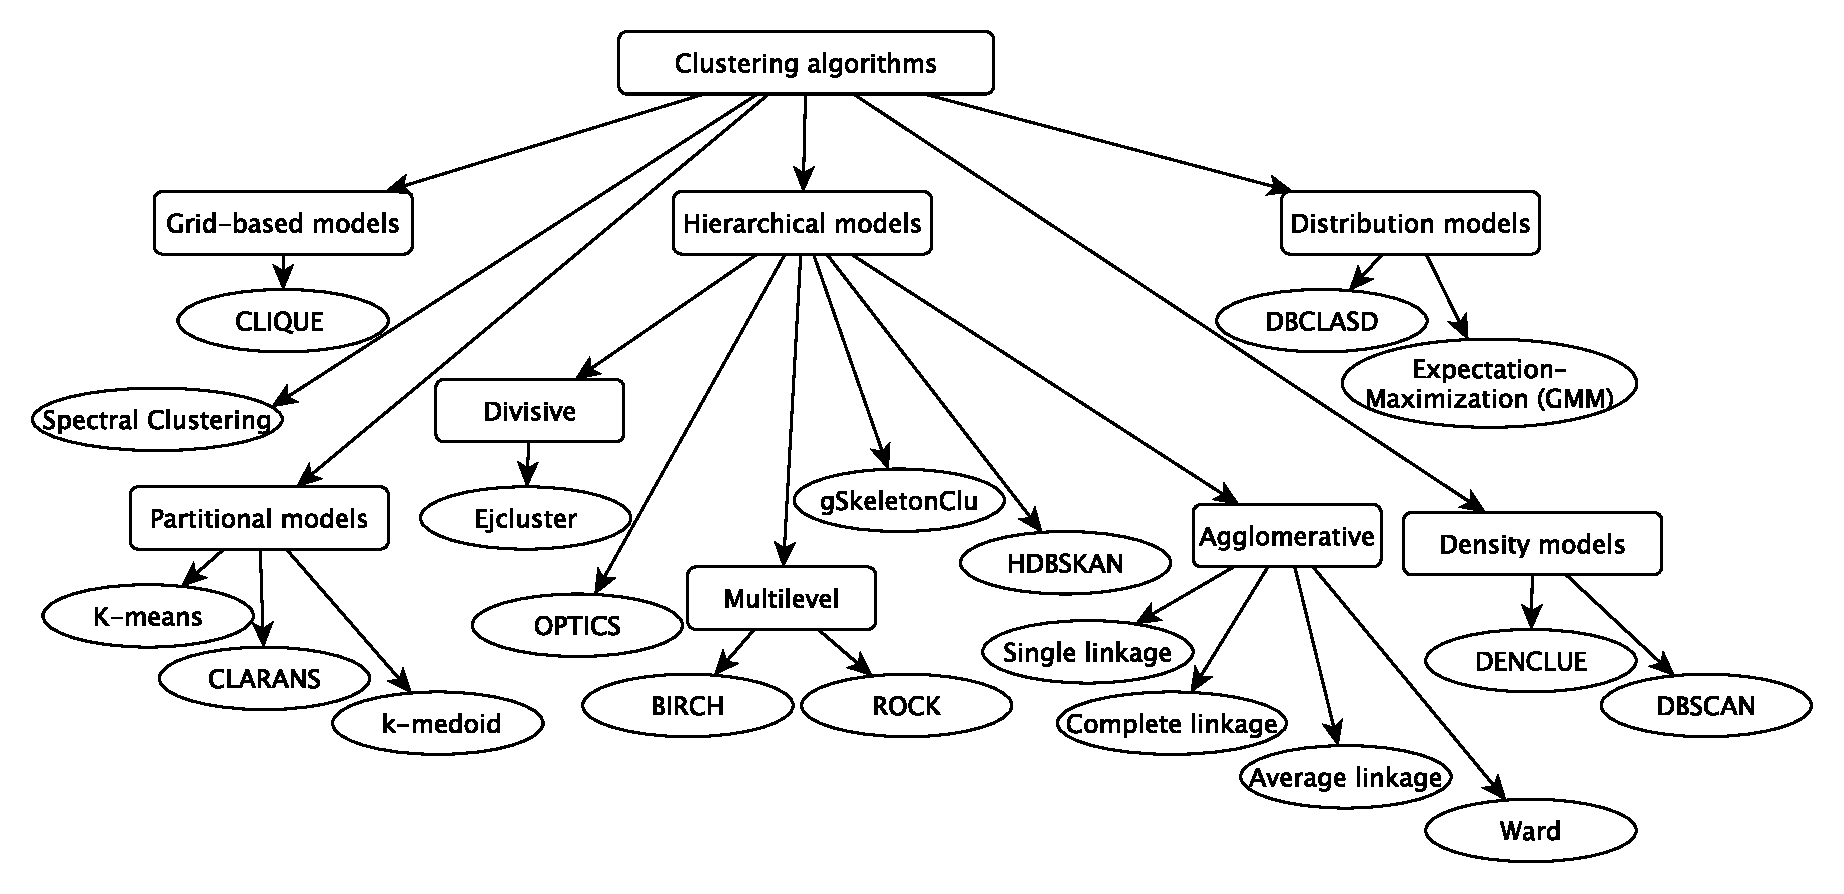
\includegraphics[width=1.0\textwidth]{Fig19.pdf}
    \caption{Taxonomy of cluster analysis techniques.}
    \label{fig:Fig19}
\end{figure}

\section{Cluster Analysis}
\label{Cluster Analysis}
Cluster analysis is a set of unsupervised machine learning techniques aimed at grouping similar in some sense objects together (in clusters). There are many ways to categorize clustering techniques based on the particular underlying approaches. One of the possible taxonomies for some techniques is depicted on~\autoref{fig:Fig19}which is partially based on a number of research on the comparison of different clustering techniques~\cite{steinbach2004challenges}~\cite{karypis2000comparison}~\cite{DBSCANvsK-Means}. Instead, the intention is to cluster financial network participants according to some attributes as good as possible. Generally, a good clustering method will produce high-quality clusters characterised by high intra-class similarity, low inter-class similarity and by some other common clustering quality evaluation metrics.

\subsection{$k$-means}
\label{k-means}
$k$-means is one of the most simple yet effective and common partitioning algorithms for solving a clustering problem in an unsupervised manner. The presumably first description of the technique dates back to 1967~\cite{k-maens1967}. It is an iterative algorithm that seeks local maxima through a sequence of iteration. $k$-means is comparatively fast technique capable of handling large data sets with the linear time complexity. However, like many other clustering techniques, it suffers from "curse of dimensionality".

The starting point and at the same time the most ambiguous step of the algorithm is determining the number of clusters hidden intrinsically in the original data. The initially chosen number could be optimized later based on elbow criterion~\cite{ElbowMethod2014}. For $k$ clusters assign randomly the cluster centroids in the data space~\autoref{fig:Fig20}.
\begin{figure}[H]
    \centering
    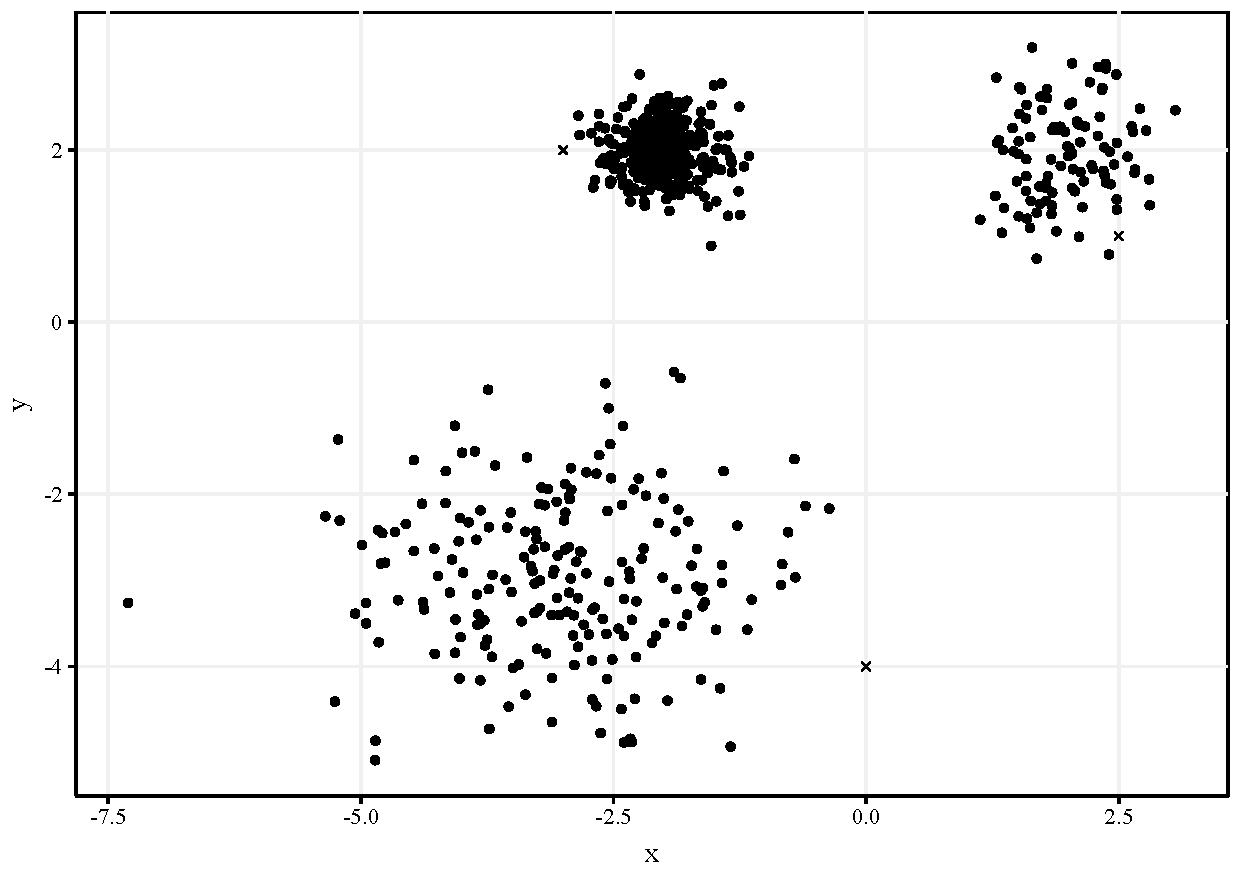
\includegraphics[width=0.65\textwidth]{Fig20.pdf}
    \caption{$k$-means clustering in 2-dimensional space. In the first iteration, the cluster centroids are randomly picked points in the space denoted by crosses on the plot.}
    \label{fig:Fig20}
\end{figure}
The next crucial step of the algorithm is to choose a proper distance measure in the given space. The common choice is to consider the Euclidean distance in a metric space. The Euclidean distance between points $\textbf{x}=(x_1,x_2,...,x_n)$ and $\textbf{y}=(y_1,y_2,...,y_n)$ in Euclidean $n$-dimensional space is defined as follows:

\begin{equation}
  d(\textbf{x,y})=\sqrt{(x_1-y_1)^2+(x_2-y_2)^2+...+(x_n-y_n)^2}
  \label{eq:equat14}
\end{equation}
Unfortunately, if the original space comprises too many dimensions, a pairwise distance ~\autoref{eq:equat10} involves an increasing number of addends under the square root and after its extraction leads to pretty much similar distances between all points in the space - an implication of the "curse of dimensionality". To overcome this flaw it is recommended to reduce the dimensionality of the space before clustering as described in \ref{Dimensionality Reduction}.

The next step is to assign the data points to one of the clusters. The affiliation to the cluster is measured by the distance between a point and a cluster centroid. The smallest distance to a centroid indicates the point's cluster at the current iteration. Once all points are assigned to some cluster, recompute new cluster centroids as the centre of mass among cluster members. Start the next iteration by placing new centroids and repeat the procedure again until the location of centroids will minimize the sum of squared distances from the cluster points~\autoref{fig:Fig21}.
\begin{figure}[H]
    \centering
    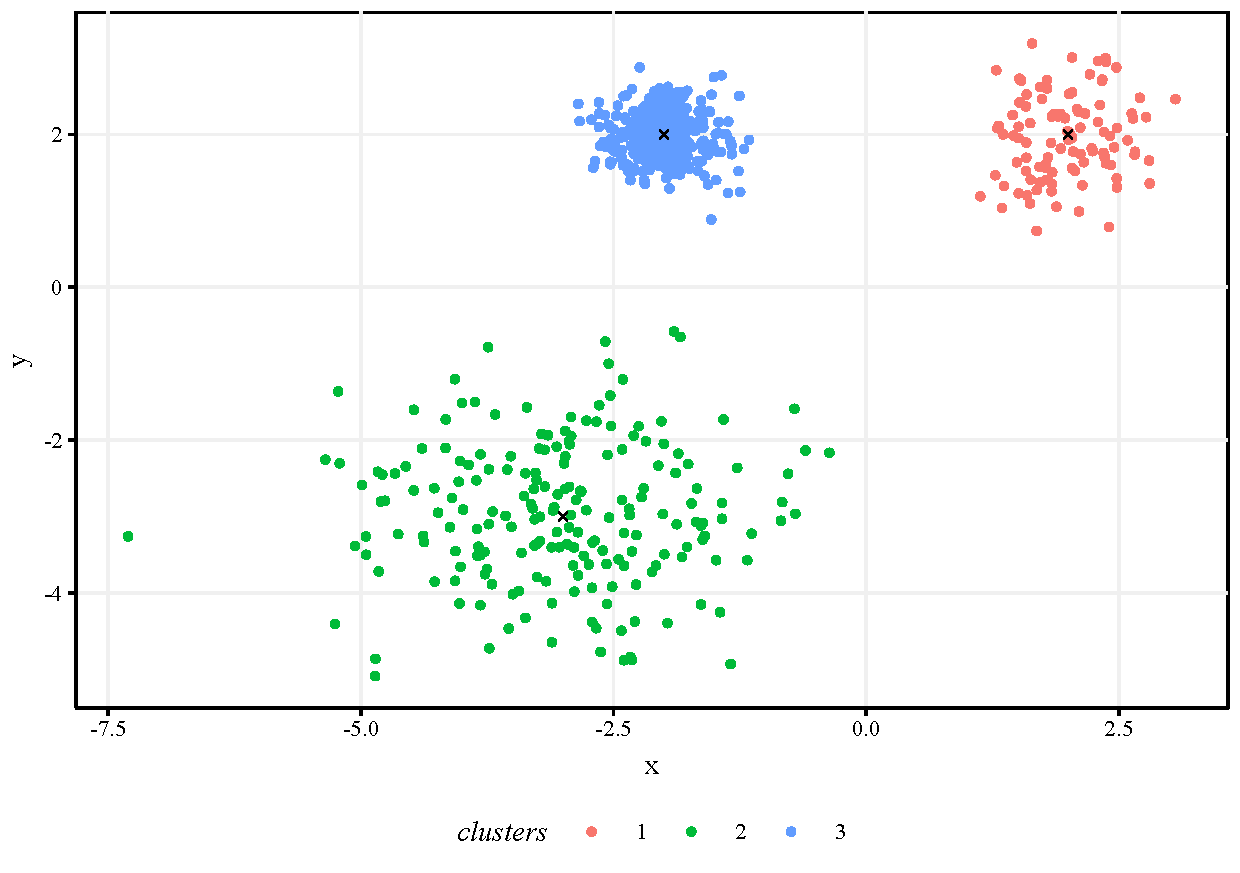
\includegraphics[width=0.65\textwidth]{Fig21.pdf}
    \caption{$k$-means clustering in 2-dimensional space. At the first iteration, the cluster centroids are randomly picked points in the space denoted by crosses on the plot.}
    \label{fig:Fig21}
\end{figure}

The ultimate goal of $k$-means clustering is to minimize total intra-cluster variance. Therefore the objective is represented by the squared error function and looks as follows:
\begin{equation}
  C = \sum_{j=1}^{k} \sum_{i=1}^{n}||x_i^{(j)}-c_j||^2
  \label{eq:equat15}
\end{equation}
where $k$ is a number of clusters, $n$ is a number of data points, and $c_j$ is a centroid of cluster $j$. The optimal number of clusters $k$ assures the best data points separation and minimizes $C$.

In practice, there is usually no prior information about the magnitude of $k$. However, the optimal value could be approximated by comparing the outcomes of multiple runs setting with different $k$. A run with the smallest $C$ usually accounts for the best $k$. It's crucial to treat large values of $k$ carefully. Although they may seem like the best choice in terms of decreasing the error $C$, they often increase the risk of overfitting.

\textbf{Limitations. }
The considerable challenge in $k$-means clustering in practice is a preliminary choice of the number of clusters assumed in the original data. There is no solid theoretical approach to define the optimal number of clusters, nevertheless, there are some methods in practice that may help. The elbow method described in ~\cite{ElbowMethod2014} focuses on  the percentage of variance explained as a function of the number of clusters. The idea of the method is to increment $k$ until adding one more cluster doesn't lead to much better modelling of the data. ~\autoref{fig:Fig22} shows the elbow plot for data points from ~\autoref{fig:Fig21}. The first three clusters along the $x$ axis add the most of information but further increasing does not contribute much. Thereby, the angle ("elbow") formed at the third cluster is considered the optimal point to derive $k$. 

\begin{figure}[H]
    \centering
    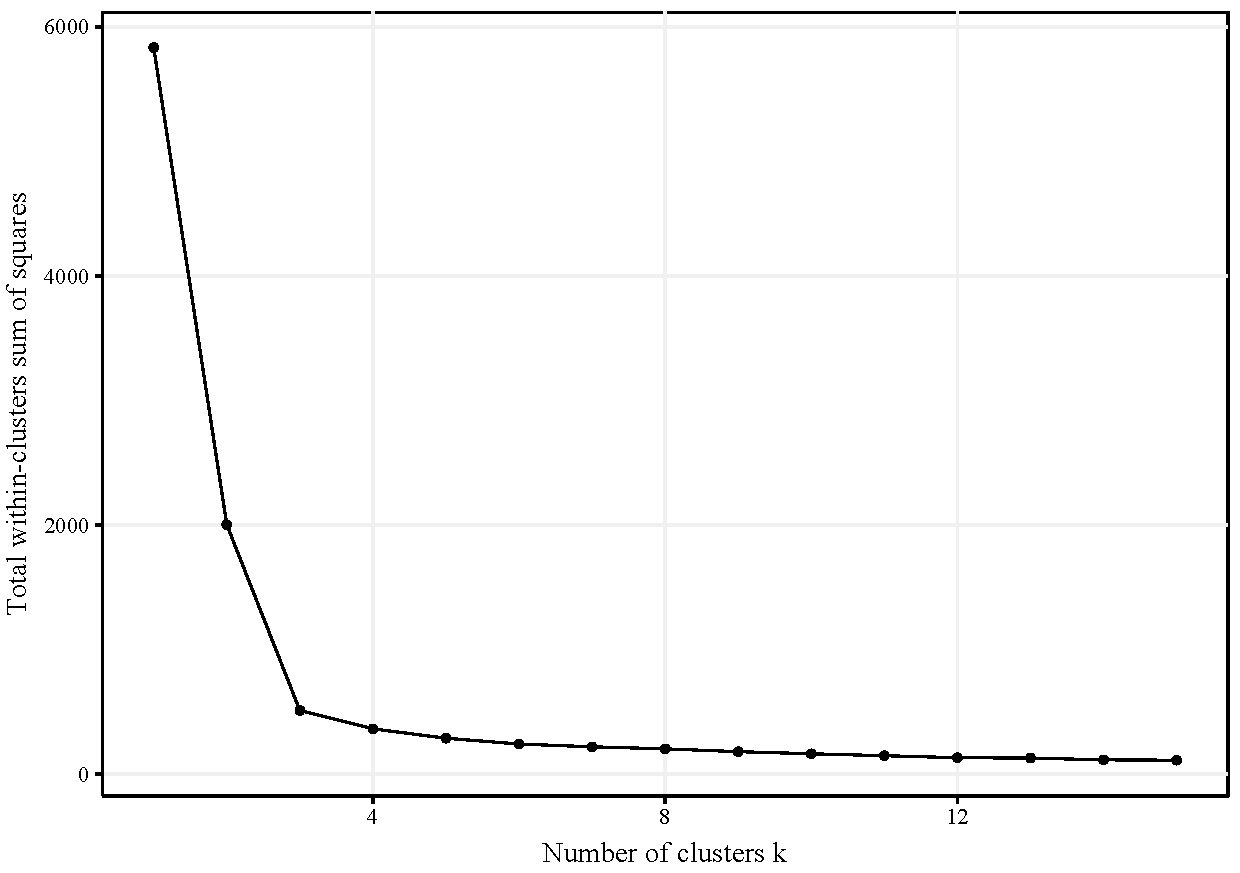
\includegraphics[width=0.5\textwidth]{Fig22.pdf}
    \caption{Elbow plot for the data points from ~\autoref{fig:Fig21}. Three clusters are the optimal choice for the data set.}
    \label{fig:Fig22}
\end{figure}

$k$-means clustering is the stochastic algorithm as the initial centroids are placed at random. Even under preserving the same number of clusters, the algorithm may lead to different outcomes. It is especially common for real-world data. The problem of stability of $k$-means clustering is explored among others in ~\cite{ClusterStability2007}. The common way to identify the stable clusters in practice is to run clustering multiple times and choose the most frequent separation.

Another weakness of the method is an assumption of certain cluster shape (e.g. hyper spherical in a metric space with Euclidean distance). $k$-means is incapable to find bent, S-shaped clusters, or rings.

\subsection{Hierarchical DBSCAN}
Density-Based Spatial Clustering of Applications with Noise in 1996 ~\cite{DBSCAN} in contrast to $k$-means is designed to discover clusters of arbitrary shape. Similar to $k$-means it allows any distance metric, is efficient for large data sets and requires two user-defined input parameters: a maximum radius of the local neighbourhood $Eps$ and a minimum number of points fall in the neighbourhood $MinPts$ that can be reduced to the only last. A density-based notion from ~\cite{DBSCAN} defines a cluster as a maximal set of density-connected points. The significant advantage over $k$-means is that there is no need to set a number of clusters a priori. DBSCAN produces clusters based on the intrinsic structure of the original data.

Hierarchical DBSCAN is a DBSCAN extension first proposed in 2013 ~\cite{HDBSCAN}. Unlike DBSCAN generalization of parameters $Eps$ and $MinPts$ over all clusters, HDBSCAN allows finding clusters of varying densities by performing DBSCAN over varying $Eps$ values and subsequent result integration. This also leads to a more robust parameter selection and overall cluster stability. 

DBSCAN is not hierarchical and finds only "flat" clusters, while density-based hierarchical algorithms like HDBSCAN and OPTICS~\cite{OPTICS1999Ankerst} produce a nested cluster hierarchy. In the case of the second, it creates a cluster-ordering corresponding to many density-based clusterings according to a broad range of parameter settings and then applies a global cut/density threshold to produce "flat" clusters. This strategy may not result in the optimal set of clusters characterized by different density levels.

The main innovation introduced by HDBSCAN creators in~\cite{HDBSCAN} is an automatic method to extract a flat clustering solution based on local cuts applying to a single-linkage-like dendrogram tree in hierarchical clustering in order to extract the most significant clusters. HDBSCAN aims at finding stable clusters by optimizing an objective function to retrieve a global optimum for stability.

The algorithm starts with the assumption of having noise in real data that typically reside in areas of low density. The simplest and parsimonious way to distinguish clusters of higher density from sparsely distributed noise is to consider a distance between the $k$ nearest neighbours in a metric space. Assume $k$ = 5 neighbours surrounding a source point in a metric space, then the \textit{core distances} of randomly chosen points $a$ and $b$ are $core_{k=5}(a)=r1$ and $core_{k=5}(b)=r2$ respectively (~\autoref{fig:Fig23}).

\begin{figure}[H]
    \centering
    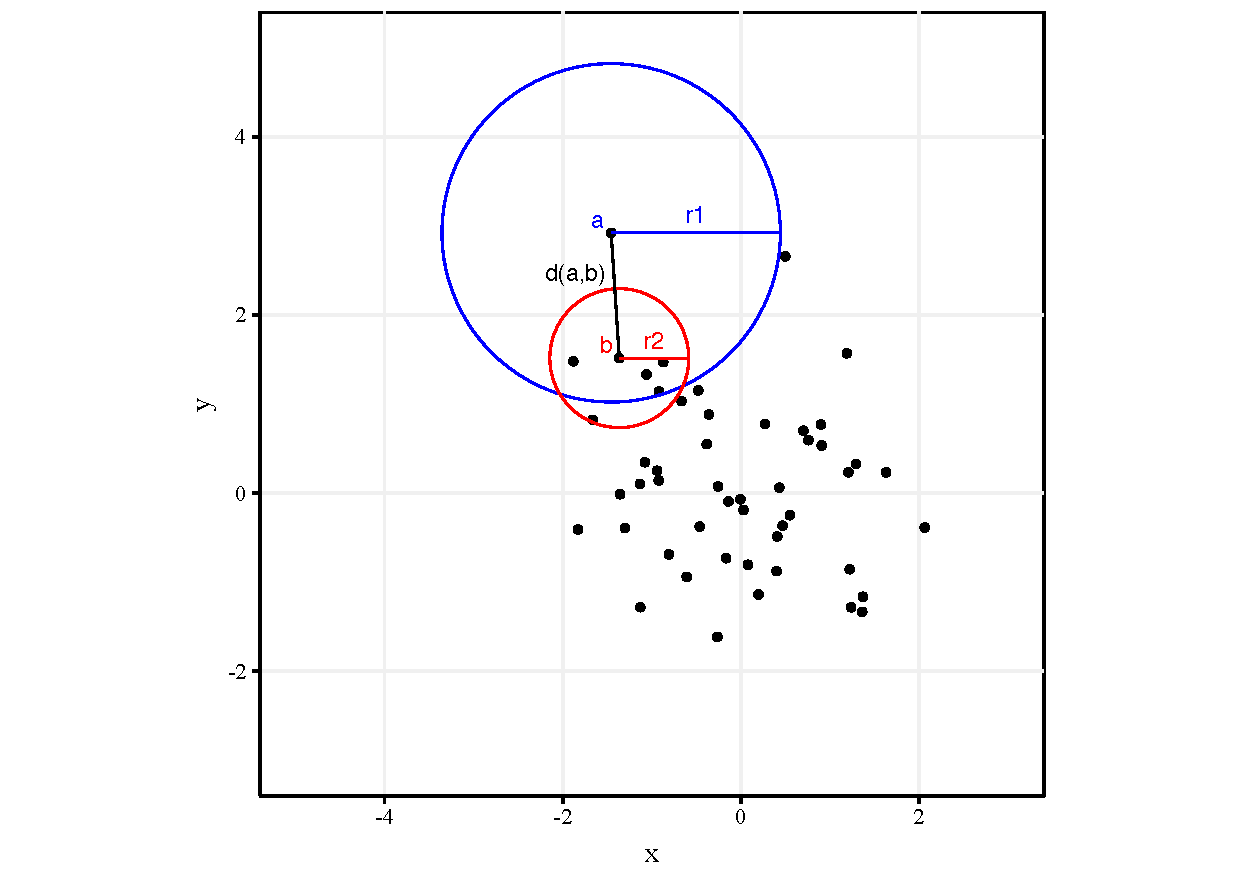
\includegraphics[width=0.55\textwidth]{Fig23.pdf}
    \caption{Core distance of a point is the radius of circumference spanning 5 nearest neighbours with the centre in the source point.}
    \label{fig:Fig23}
\end{figure}

To spread apart points of potential clusters and noise Ricardo J. G. B. Campello et al. proposed to use a \textit{mutual reachability distance}, which is defined for $a$ and $b$ from~\autoref{fig:Fig23} as follows:
\begin{equation}
  d_{m_r_d}(a,b)=max\{core_{k}(a), core_{k}(a), d(a,b)\}
  \label{eq:equat16}
\end{equation}
where $d(a,b)$ is the original metric distance between $a$ and $b$.~\autoref{eq:equat16} suggests preserving the original distance between densely placed points which core distances are smaller than pairwise and this way pushing away sparser points while increasing the pairwise distance to the largest core distance. Therefore, the point $a$ from~\autoref{fig:Fig23} will be pushed away from the denser cluster because $d_{m_r_d}(a,b) = core_{k}(a)$. This approach results in the enlarging margins around dense clusters, however, the choice of $k$ should be prudent: the larger magnitudes lead to more points on cluster borders will be considered as noise.

The next step is to derive the minimum spanning tree of the weighted graph where vertices are data points and an edge between any two points has weight equal to its mutual reachability distance~\autoref{fig:Fig24b}. A complete graph has $n^2$ edges which makes it slow to process while searching for a minimal set of edges connecting all nodes. One of the efficient algorithms for retrieving spanning tree from a connected graph is a Prim–Jarník greedy algorithm\footnote{\textbf{Prim–Jarník algorithm} finds a subset of the edges that forms a tree that includes every vertex where the total weight of all the edges in the tree is minimized. Source: https://www.wikipedia.org}. It finds a minimum spanning tree for a weighted undirected graph and was proposed in 1930 by Vojtěch Jarník~\cite{Jarnik1930SpanningTree} and later rediscovered by Robert C. Prim in 1957~\cite{Prim1957SpanningTree}.

\begin{figure}[H]
    \centering
    \begin{minipage}{0.42\textwidth}
        \centering
        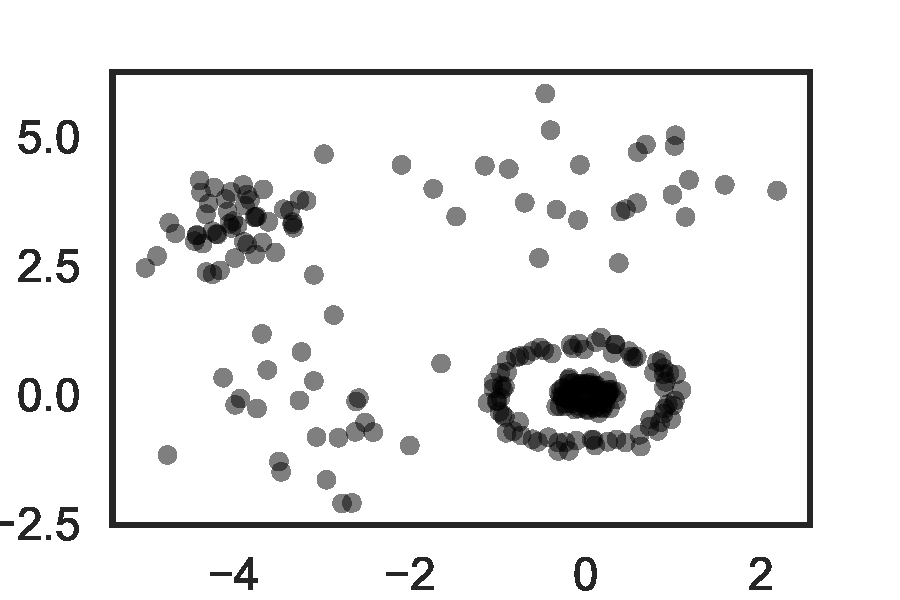
\includegraphics[width=0.9\textwidth]{Fig24a.pdf}
        \caption{Points in the original space.}
        \label{fig:Fig24a}
    \end{minipage}\hfill
    \begin{minipage}{0.42\textwidth}
        \centering
        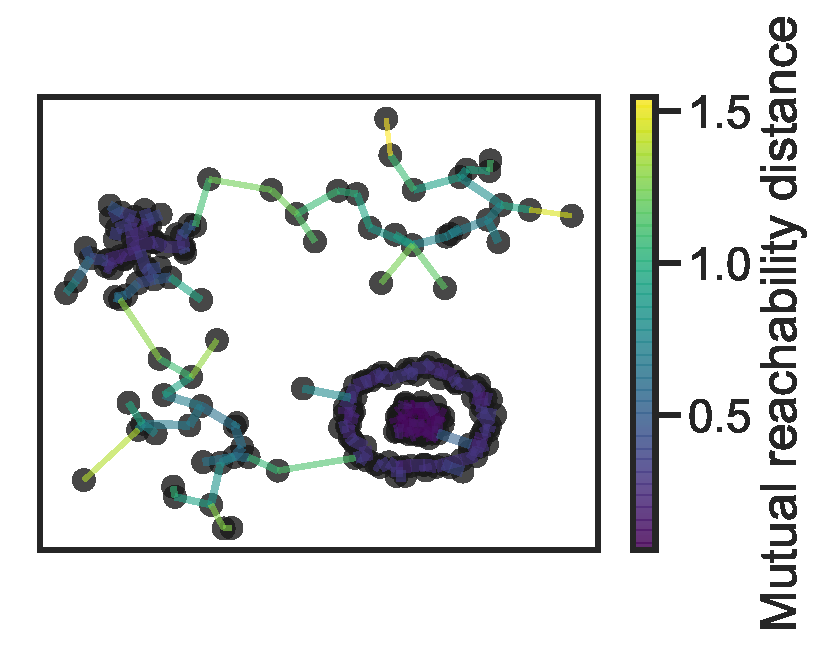
\includegraphics[width=0.9\textwidth]{Fig24b.pdf} 
        \caption{Minimum spanning tree of weighted graph.}
        \label{fig:Fig24b}
    \end{minipage}
\end{figure}
\begin{figure}[H]
    \centering
    \begin{minipage}{0.42\textwidth}
        \centering
        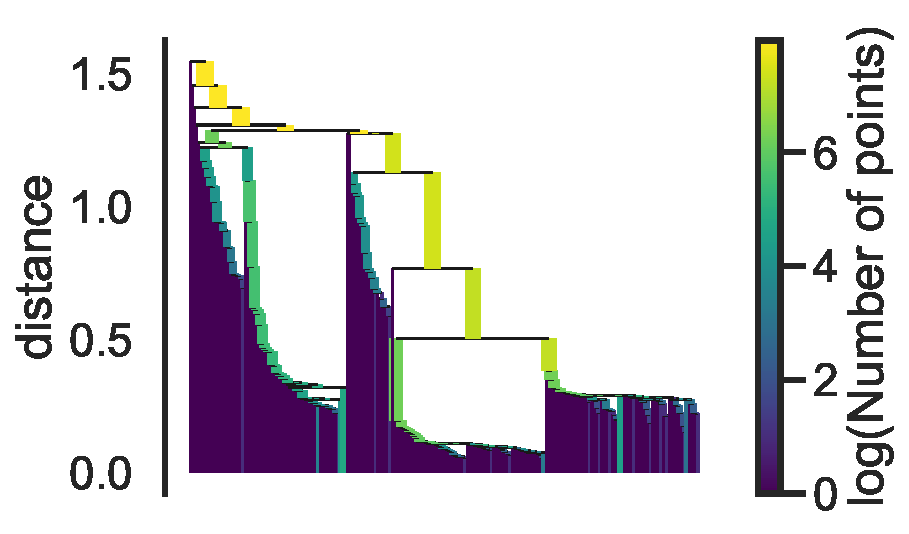
\includegraphics[width=0.9\textwidth]{Fig24c.pdf}
        \caption{Hierarchical dendrogram on mutual reachability distance.}
        \label{fig:Fig24c}
    \end{minipage}\hfill
    \begin{minipage}{0.42\textwidth}
        \centering
        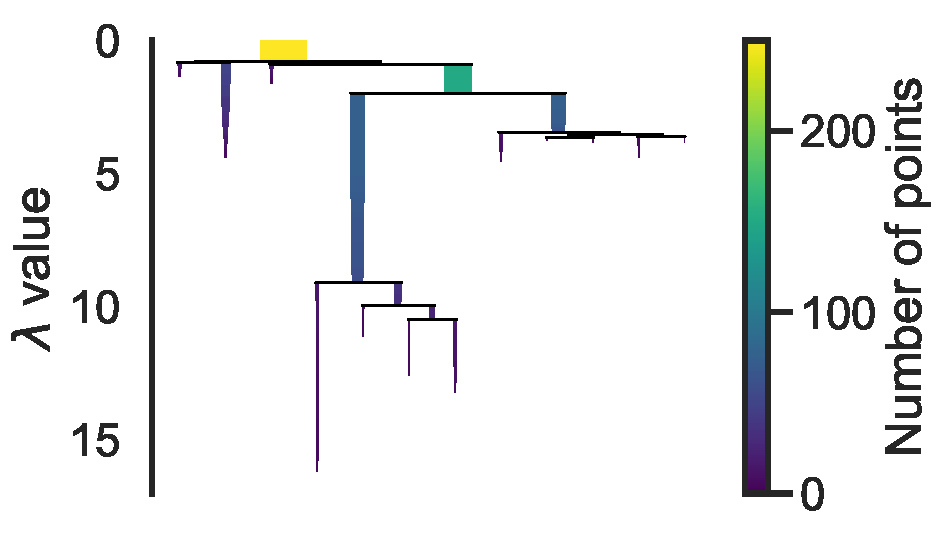
\includegraphics[width=0.9\textwidth]{Fig24d.pdf} 
        \caption{Condensed dendrogram tree without noise points (k = 5)}
        \label{fig:Fig24d}
    \end{minipage}
\end{figure}

A minimum spanning tree serves for producing a cluster hierarchy in the form of a dendrogram~\autoref{fig:Fig24c}. The next intuitive step is to infer a set of flat clusters from a dendrogram. A vast majority of hierarchical clustering techniques suggest determining a single horizontal cut level~\cite{DBSCAN}~\cite{OPTICS1999Ankerst}. However, a global cut on a single density level does not guarantee the best separation among clusters of variable density. 

To distinguish clusters points from noise, HDBSCAN algorithm relies on the user-defined parameter \textit{minimum cluster size}. It facilitates clusters search in the dendrogram: if a number of points falls apart from a cluster lower than minimum cluster size, they will be considered as noise instead of an independent cluster. On the other hand, if a split divides the cluster into two of size exceeding or equal to minimum cluster size, the split is considered as a true cluster split. This heuristic is used to truncate the dendrogram tree by eliminating noise points. After traversing the tree, the only clusters of the sufficient size persist and the rest of the points are discarded. This makes original dendrogram tree thinner like on~\autoref{fig:Fig24d} where minimum cluster size $k$=5. Here the width of the lines represents the number of points in the cluster and the pointed leaves show when noise points fall out of the clusters over the increase of mutual reachability distance.

The innovative part of the algorithm is a heuristic on an unequivocal choice of stable, long-lived, "flat" clusters. For each point of each cluster in a condensed tree on ~\autoref{fig:Fig24d} assume $\lambda_p=\frac{1}{distance_p}$ equal to reciprocal of mutual reachability distance at which that point fell out of the cluster. Additionally, for each cluster assume $\lambda_{birth}$ and $\lambda_{death}$ are equal to reciprocals of mutual reachability distance when a new cluster splits off from its parent and when a cluster splits into smaller clusters respectively. For a particular cluster $\lambda_{birth}< \lambda_p <\lambda_{death}$ and its cluster stability measure is calculated as follows:

\begin{equation}
  S = \sum_{p\in cluster}(\lambda_p - \lambda_{birth})
  \label{eq:equat17}
\end{equation}
The measure is calculated for each cluster bottom-up starting with the leaf-clusters. If the sum of the stabilities of the child clusters surpluses parent stability, then assign this sum to the parent stability. Otherwise, if the parent stability is greater than the sum of its children stabilities, then include this cluster in the final set of "flat" clusters and exclude all its descendants. Continue the process until reaching the root, then traverse tree top-down and collect the selected "flat" clusters as ~\autoref{fig:Fig25} illustrates.
\begin{figure}[!hp]
    \centering
    \begin{minipage}{0.42\textwidth}
        \centering
        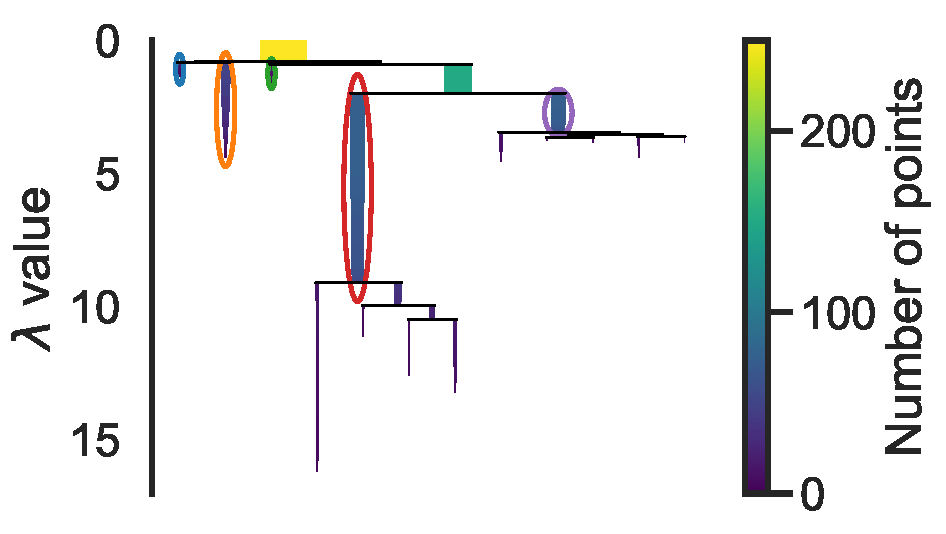
\includegraphics[width=0.9\textwidth]{Fig25.pdf}
        \caption{Selected "flat" clusters in the condense tree.}
        \label{fig:Fig25}
    \end{minipage}\hfill
    \begin{minipage}{0.42\textwidth}
        \centering
        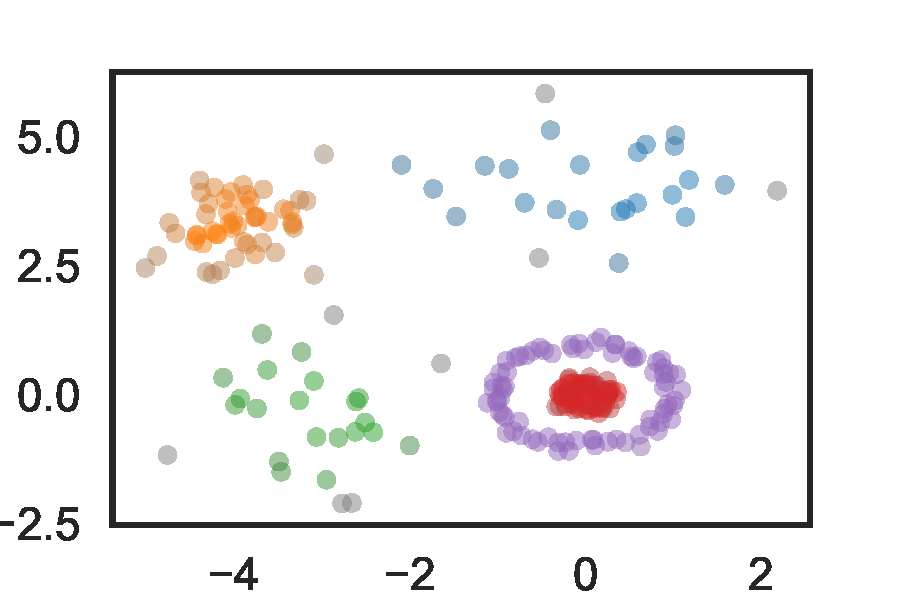
\includegraphics[width=0.9\textwidth]{Fig26.pdf} 
        \caption{Points labelled by HDBSCAN-defined cluster membership.}
        \label{fig:Fig26}
    \end{minipage}
\end{figure}

The result on ~\autoref{fig:Fig26} demonstrates that the proposed density-based hierarchical clustering algorithm is capable to find clusters of varying density along with clusters of arbitrary shapes like a ring and distinguish them from detached noise points.

\section{Cluster evaluation strategies}
\label{Cluster evaluation strategies}
A clustering evaluation relies on assessment measures, which serve for comparing results from different clustering algorithms on one scale. The clustering evaluation is needed to compare two or more clustering algorithms, tune clustering hyperparameters and to avoid finding clusters in random data. Generally, clustering evaluation statistics are divided between two classes: internal and external. Internal measures use only internal information on clustered data to evaluate the goodness of clustering, while external measures rely on externally provided ground truth labels. This section will discuss several internal clustering evaluation measures for unsupervised clustering.

\begin{enumerate}
  \item \textit{Root-mean-square standard deviation index (RMSSTD)}~\cite{sharma1996RMSSDT} measures the homogeneity of the clusters. In essence, it is a square root of the pooled sample variance of all variables.
      \begin{equation}
    RMSSTD = \sqrt{\frac{SS_1+...+SS_p}{df_1+...+df_p}}\;,\;\;\; where\;SS_j = \sum_{i=1}^{n}(x_{ij}- \boldsymbol{x_j} )^2
    \label{eq:equat18}
    \end{equation}
  where $p$ is a number of clusters, $SS_j$ is the within sum of squares of the $j$-th variable. The low RMSSTD values testify the high within-clusters homogeneity and hence a better clustering.
  
  \item \textit{R-square index (RS)}~\cite{sharma1996RMSSDT} measures the extent to which clusters are different from each other. It is a ratio of the difference between the total sum of squares and the total between sum of squares to the total sum of squares.
    \begin{equation}
    RS = \frac{SS_{total}-SS_{within}}{SS_{total}}\;,\;\; where\;SS_{total}=\sum_{j=1}^p \sum_{i=1}^n (x_{ij}-\boldsymbol{x_j})^2
    \label{eq:equat19}
    \end{equation}
  The minimum RS value 0 means there is no difference among the clusters, the maximum value 1 indicates a significant difference among the clusters.
  
  \item \textit{SD Validity index (SD)}~\cite{halkidi2000quality} relies on the average scattering of clusters and total separation of clusters. The scattering is calculated as the ratio of within-cluster variances to the variance of the data set, while the total separation of clusters is based on the distance between cluster centres $c_i$:
    \begin{equation}
        Scatt = \frac{1}{p}\sum_{i=1}^p \frac{||\boldsymbol{\sigma(c_i)}||}{||\boldsymbol{\sigma(x)}||}\;,\;\;\; Dis = \frac{\max_{i,j=1...p}||c_j-c_i||}{min_{i,j=1...p}||c_j-c_i||}\sum_{k=1}^p \bigg(\frac{1}{\sum_{\substack{j=1 \\ i\neq j}}^p ||c_j-c_i||}\bigg)
    \label{eq:equat20}
    \end{equation}
    \begin{equation}
        SD = Dis_{maximal\;p} \cdot Scatt + Dis
    \label{eq:equat21}
    \end{equation}
    The low SD Validity index values means better clustering: clusters are compact and well separated.
    
  \item \textit{S\_Dbw Validity index (S\_Dbw)}~\cite{halkidi2001S_Dbw} is based on cluster compactness and separation and, additionally, considers clusters densities. The intra-cluster variance is $Scatt$ from ~\autoref{eq:equat20}, and the inter-cluster density is defined as follows:
      \begin{equation}
        Dens\_bw=\frac{1}{p(p-1)}\sum_{i=1}^p \Big(\sum_{\substack{j=1 \\ i \neq j}}^p \frac{density(u_{ij})}{\max\{density(c_i),density(c_j)\}}\Big)
    \label{eq:equat22}
    \end{equation}
  where $u_ij$ is the middle point between clusters centres $c_i$ and $c_j$. The $density$ function counts the number of points in a hyper-sphere with radius equal to the average standard deviation of clusters ($avg\_std\_clus = \frac{1}{p}\sqrt{\sum_{i=1}^p||\sigma(c_i)||}$ ).
    \begin{equation}
        S\_Dbw=Scatt+Dens\_bw
    \label{eq:equat23}
    \end{equation}  
  It enables reliable evaluation of globular clusters. Low $S\_Dbw$ values indicate a good clustering result. 
  
  \item \textit{Silhouette coefficient (SC)}~\cite{zhu2010clustering} is a measure of how similar an object is to its own cluster compared to other clusters. The coefficient is relevant for hierarchical and partitioning clustering techniques.
    \begin{equation}
    SC = \frac{1}{n}\sum_{i=1}^n \frac{b_i - a_i}{\max\{a_i, b_i\}}
    \label{eq:equat24}
    \end{equation}
  where $a_i$ is the average distance between $i$ and all other data points in the same cluster and $b_i$ is the smallest average distance of $i$ to all points in any other cluster, of which $i$ is not a member.
      \begin{equation}
        a_i = \frac{1}{|C_i|-1}\sum_{j=C_i,i\neq j} d(i,j)\;\;\;\;\; 
        b_i = \min_{i\neq j} \frac{1}{|C_i|}\sum_{j\in C_j} d(i,j)
        \label{eq:equat20}
      \end{equation}
  where $d(i,j)$ is the distance between data points $i$ and $j$ in the cluster $C_{i}$. The SC value may vary between -1 and 1. The higher values characterizes better clustering.
  
  \item \textit{Davies–Bouldin index (DB)}~\cite{davies1979cluster} is an internal, very fast comparing to Silhouette coefficient evaluation measure calculated as follows:
    \begin{equation}
        DB = \frac{1}{|C_i|-1}\sum_{j=C_i,i\neq j} d(i,j)
        \label{eq:equat21}
     \end{equation}
  where $n$ - the number of clusters, $c_{x}$ - the centroid of cluster $x$, $\sigma _{x}$ - the average distance from all elements in the cluster $x$ to centroid $c_{x}$, and $d(c_{i},c_{j})$ - the distance between centroids $c_{i}$ and $c_{j}$.
  
  \item \textit{Dunn index (D)}~\cite{Dunn1973index} tends to identify dense and well-separated clusters by dividing the minimal inter-cluster distance by the maximal intra-cluster distance:
    \begin{equation}
        D = \frac{\min_{1\leqslant i < j \leqslantn n}d(i,j)}{\max_{1\leqslant k\leqslant n}d'(k)}
        \label{eq:equat22}
     \end{equation}  
    where $d(i,j)$ - the distance between clusters $i$ and $j$, $d'(k)$ - the intra-cluster distance of cluster $k$. Clusters with high intra-cluster similarity and low inter-cluster similarity increases Dunn index.
    
    \item \textit{Calinski-Harabasz index}~\cite{CH2007} is higher when clusters are dense and well separated. For $k$ clusters, the Calinski-Harabasz score $CH$ is given as the ratio of the between-clusters dispersion mean and the within-cluster dispersion:
        \begin{equation}
            CH(k) = \frac{Tr(\boldsymbol{B_k})}{Tr(\boldsymbol{W_k})} \times \frac{N-k}{k-1}
            \label{eq:equat23}
         \end{equation}
     where $N$ is the number of the data points, $\boldsymbol{B_k}$ is the between-clusters dispersion matrix and $\boldsymbol{W_k}$ is the within-cluster dispersion matrix defined as:
        \begin{equation}
            \boldsymbol{B_k} = \sum_q n_q(c_q-c)(c_q-c)^T\;\;\;\; \boldsymbol{W_k} = \sum_{q-1}^k \sum_{x \in C_q} (x-c_q)(x-c_q)^T
            \label{eq:equat24}
        \end{equation}
    with $C_q$ - the set of points in cluster $q$ , $c_q$ - the center of cluster $q$, $c$ - the center of dataspace $E$, and $n_q$ - the number of points in cluster $q$.
\end{enumerate}

\section{Financial Networks}
\label{Financial Networks}
During the last decades, a concept of financial network has been actively exploited for studying the rapidly evolving global interconnected financial system. The major areas where the concept has already proved its utility are financial contagion and systemic risk~\cite{ContagionFinNets} ~\cite{ResContagionFinNets} ~\cite{NetStrucSysRiskBankSys}. Such detrimental phenomena as the common shock propagation, the unfolding of default cascades, and the domino effects of insolvency motivated many researchers to use the financial network model to track a spillover effect. Other areas, where the financial networks have recently come into play are stock market analysis~\cite{NetAnalysisChineseStockMarket} ~\cite{StatisticAnalysisFinNetworks}, formation of interbank markets, assessing stability of financial systems, fraud and anomalies detection~\cite{AnomalyNetIntrusion}, and much more.

Unfortunately, there are not so many publicly-available researches exploring real-world transaction data because of the highly sensitive nature of the data. However, the enormous recent popularity of decentralized platforms based on blockchain technology launched fresh incentives in financial networks studies. A great variety of cryptocurrencies attracted attention of many investors due to real-time transparent maintaining of a public digital ledger of transactions, which is considered to be incorruptible~\cite{miraz2018applications}.

This fact spawned a lot of different financial transaction networks built on mutual trust where the value of an asset is defined by supply and demand similar to a state currency in a bank transaction. Some research on characterizing such networks have been recently done all over the world ~\cite{victormeasuring}, ~\cite{BlockchainGraph}, ~\cite{miller2015discovering}.

Despite the lack of publicly available data from financial institutions to dissect financial network phenomena, there are some studies based on real-world data. Comprehensive research of the real-world transaction data disclosed by Bank of Japan in 2004 ~\cite{inaoka2004fractal} detected a fractal structure of the dynamic network formalized from the set of transactions between financial institutions. The behaviour of financial players in Austria was studied in 2009 by exploring a topology of the network, in which accounts are represented as nodes and transactions are weighted edges between the nodes~\cite{Kyriakopoulos2009}.

\section{Summary}
The current chapter covered all existing techniques, that are used in the concept of the thesis. These techniques have been provided with illustrated explanations, known limitations and references to authors and related works. The next chapter gives an understanding how the discussed methods are applied in the context of the current work.

\chapter{Concept and Design}
\label{cha:conceptanddesign}

This chapter focuses on the central concept for user segmentation in financial transaction networks. It is designed in the form of a data science pipeline, which consists of three primary stages of data processing. The purposes and contents of each stage will be covered below in detail. 

One of the main contributions of the current thesis is the first stage of the pipeline. It is represented by new modification of Node2vec framework for unsupervised network feature engineering taking into account dynamic nature of a network and remote structural homogeneity. The stage will be discussed and explained in this chapter with illustrations to allow a reader to fully comprehend the idea. The second stage of the data processing pipeline reduces dimensions of the data and serves as a preparation for the third final stage. The third stage is clustering in the low-dimentional feature space. Each stage was implemented as a set of relevant unsupervised or semi-supervised state-of-the-art machine learning techniques, which led to branch structure of the pipeline. The output is the set of clusters achieved the best magnitudes of the evaluation measures among different pipeline's branches.

The basic requirements for the user segmentation pipeline are listed below:
\begin{itemize}
  \item The pipeline should be able to read and process the network data from anonymized financial transaction data set with time and result into a set of clusters of similar users. 
  \item The pipeline should consider structures of the local neighbourhoods of the users, time of committed transactions and the global structural attribute of the underlying network.
  \item The pipeline should provide several techniques at each processing stage and output clusters evaluation values from every possible successive combination of techniques (branch).
\end{itemize}

\section{Concept}
\label{Concept}
~\autoref{fig:Fig28} depicts the main stages of the concept. The input data should be in the form of a structured set of transactions with the minimum required fields: sender, receiver and time. The network embedding learning framework consumes the input data and outputs a set of derived features describing each node from the initial network. The network embedding learning stage exploits the general Node2vec framework with a modified sampling strategy. The modification incorporates graph attributes into the existing Node2vec network embedding framework. Specifically, the edge-based time (from here and further - \textit{time component}) and node-based degree (from here and further - \textit{global structural component}) attributes of the graph are incorporated into semi-random walk samples consisted of the nodes from local neighbourhoods (from here and further - \textit{local structural component}). The three components could be taken pairwise or all together for producing nodes features. The precise process of walks mining will be described below in~\ref{Automated Feature Learning Framework}. 

The output of the network embedding learning stage serves as an input for the next stage of dimensionality reduction. The second stage applies dimensionality reduction techniques to the feature set. It produces three new reduced data sets by three different dimensionality reduction techniques. At this stage, the original PCA, t-SNE, and UMAP approaches are used without modifications. The final stage consumes the low-dimensional output of the previous stage and applies cluster analysis. Cluster analysis is realized by two different clustering techniques: partitional clustering k-means and density-based clustering HDBSCAN. Both of them work well in low-dimensional metric spaces and output clusters of users based on their proximity.
\begin{figure}[!ht]
	\centering
	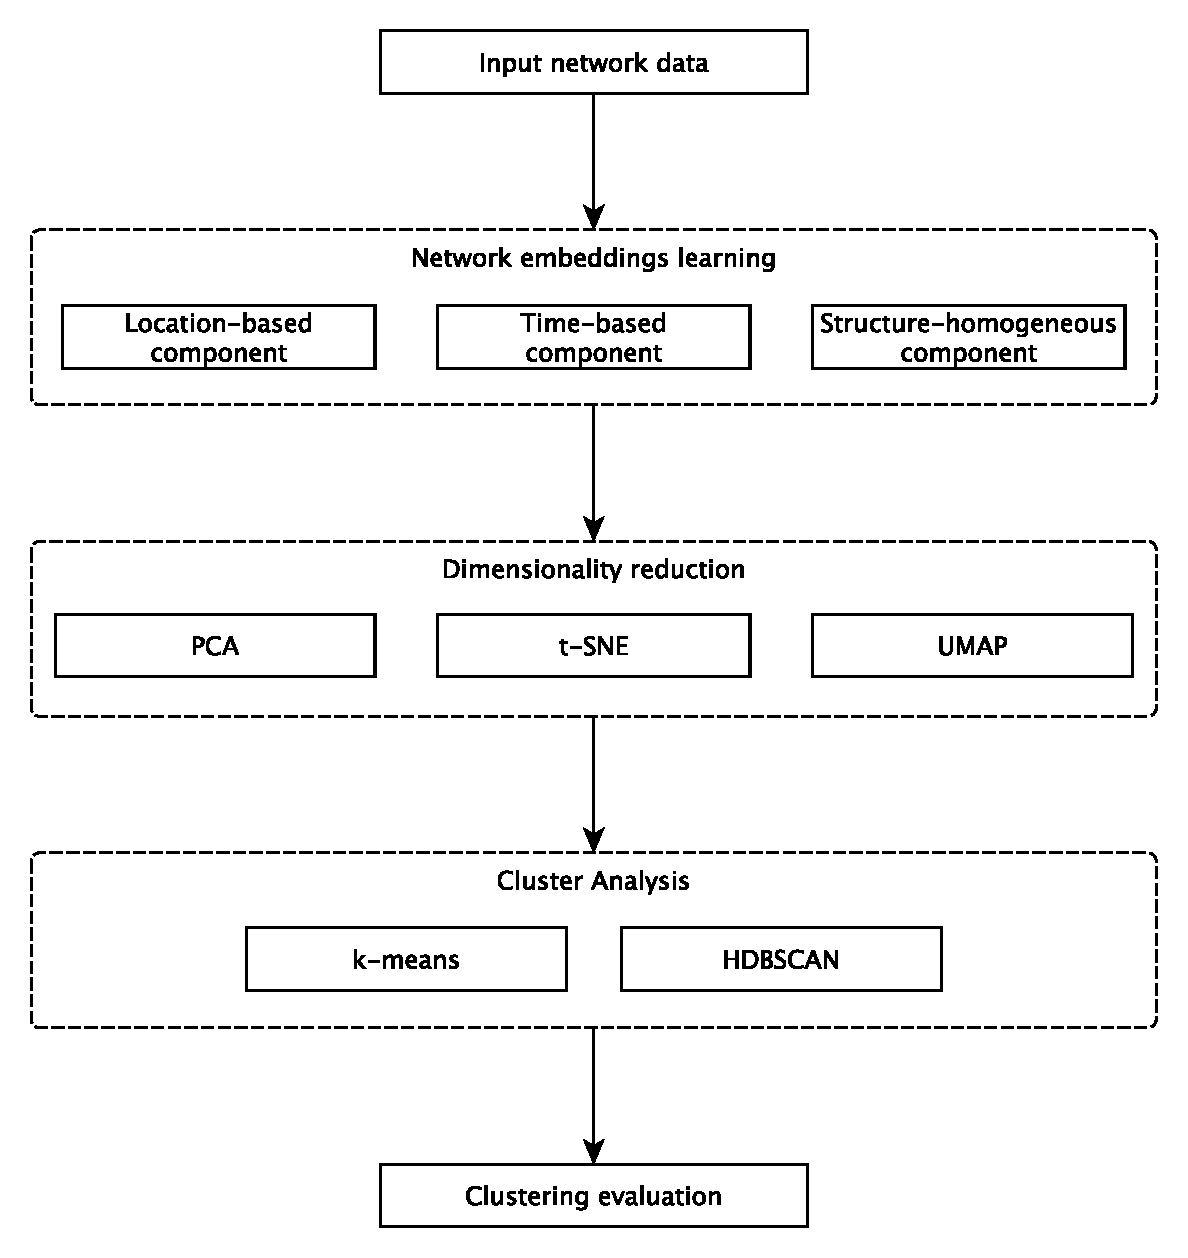
\includegraphics[width=0.7\textwidth]{images/Fig28.pdf}\\
	\caption{Concept of unsupervised data science pipeline for user segmentation in financial transaction networks.}
	\label{fig:Fig28}
\end{figure}

\section{Data preparation}
\label{Data Preparation}
Despite the input data structure is reasonably simple and requires the minimal feature set (sender, receiver, time), some pre-processing procedures have to be done as the input data preparation step for data analysis.

\subsection{Time classes}
The analysis involves time component. Transaction data sets usually contain timestamps for every transaction that are almost always unique with rare exceptions. As the goal is to place "time-similar" users closer together, i.e. the users acting at the same time period, it is reasonable to combine unique timestamps into periods. It allows to consider the users which act at the same time being more related to each other. To realize this strategy the entire time span has to be divided into consecutive time periods - time classes. Time classes have an equal length in time and do not overlap as~\autoref{fig:Fig29} shows. A particular time class can contain an arbitrary number of timestamps depending on the original data set and the time span split. The number of time classes is a user-defined parameter that can be tuned in the beginning. This pre-processing procedure results in every transaction belong to a particular class based on its timestamp.

\begin{figure}[!ht]
	\centering
	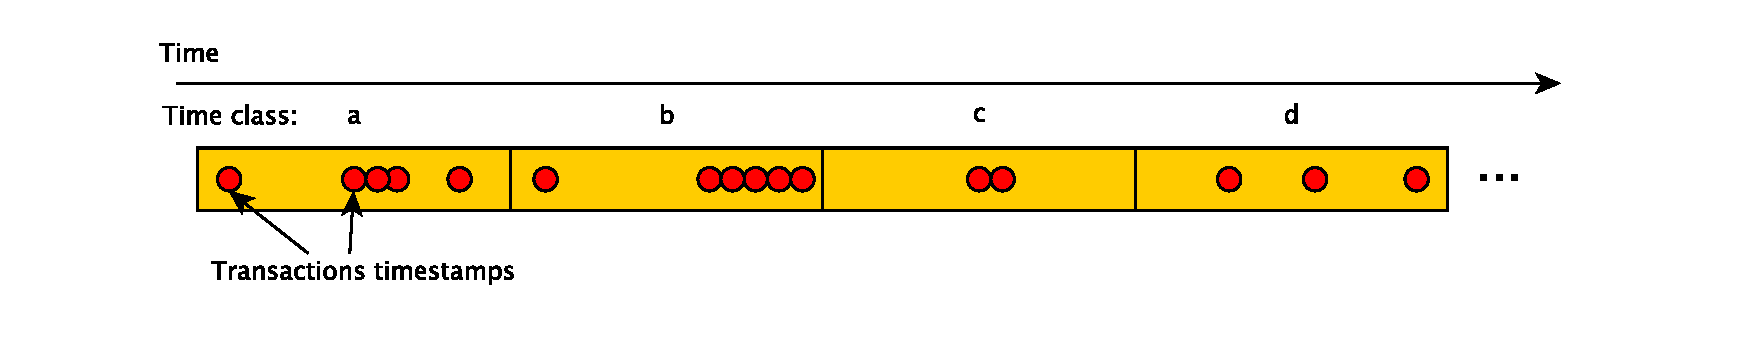
\includegraphics[width=0.95\textwidth]{images/Fig29.pdf}\\
	\caption{Transactions timestamps fall into the non-overlapping, equal-length time classes.}
	\label{fig:Fig29}
\end{figure}

\subsection{Degree classes}
Besides time, the analysis involves the degree of nodes in a network. 
It is easy and relatively fast to extract nodes' degree from a network of any size. Degree distribution of a real-world network commonly follows a Power law distribution. Thus, nodes with low degrees prevail over others. In contrast, a few nodes falling into the long tail of the distribution have high degrees and distributed sparsely. This fact suggests to group several high degrees to a degree class. A low degree can compose a degree class only by itself since a sufficient amount of nodes in a network have this degree. The number of nodes in the degree classes is determined based on considerations of the final clustering granularity. The more classes are allocated, the more clusters may be expected. 

Meaning of the global structural component is in distinguishing hubs of the highest degrees from end-points of degree one on a network's periphery. These two extrema lay on the opposite ends of the scale, while in-between there are two-degree nodes serving as bridges and other. This is another heuristic used for choosing degree classes. If there is a particular interest in participants with a certain number of established connections in a network, degree classes can be allocated in a way to capture them together. The number of degree classes is a user-defined parameter that can be tuned in the beginning. During this pre-processing procedure, every node is assigned to some degree class based on its degree.

\section{Automated feature learning framework}
\label{Automated Feature Learning Framework}
The previous section~\ref{Data Preparation} describes the data pre-processing procedures to comply with the input data format required by the automated feature learning framework. The network feature learning stage of the pipeline uses the Node2vec framework discussed in detail in the chapter~\ref{Node2vec}. The semi-random walk model of Node2vec generates ordered sequences of nodes' ids. However, unlike original Node2vec, the current framework modifies the sequences before submitting them as an input to a skip-gram model. Besides nodes' ids, the modified ordered sequences contain the time component represented by time classes of transactions and the global structural component defining the homogeneity of remote users over the network. The next two subsections will cover the imputations of time and degree to sequences of nodes' ids.

\subsection{Time component}
\label{Time component}
The Node2vec framework learns representations of network nodes in some feature space by sampling nodes' local neighbourhoods in the form of ordered sequences of nodes' ids. By nature, a time class in the prepared input data is defined for a transaction and not for a user represented by a network node. A transaction consists of two users: sender and receiver. To enable a skip-gram model to study a node representation from both its local neighbourhood and the time classes of transactions between nodes within this local neighbourhood, the ordered sequence should contain both nodes' ids and time classes.~\autoref{fig:Fig30} shows how an ordered sequence of nodes' ids alternated with time classes of intermediate transactions (bottom) can be obtained from a Node2vec semi-random walk sampled from a transaction graph (top).
\begin{figure}[!ht]
	\centering
	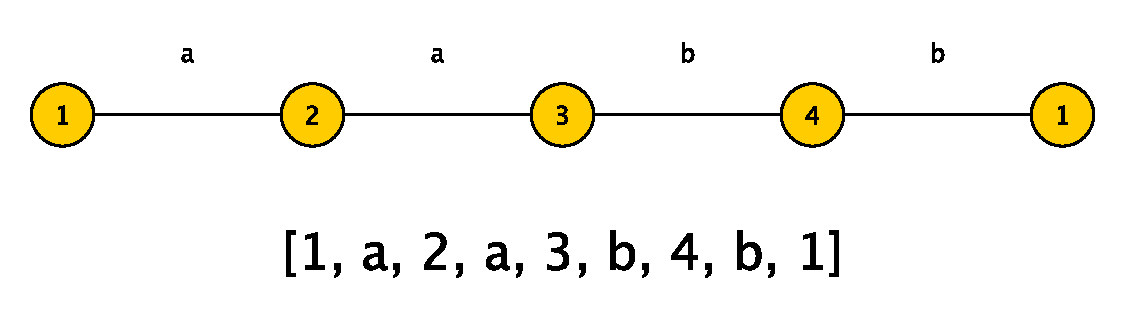
\includegraphics[width=0.5\textwidth]{images/Fig30.pdf}\\
	\caption{Top: Node2vec semi-random walk sampled from a transaction graph. Bottom: ordered sequence of nodes' ids and time classes of intermediate transactions.}
	\label{fig:Fig30}
\end{figure}

The ordered sequence on~\autoref{fig:Fig30} indicates that nodes 1, 2, 3, 4 are in the same neighbourhood, nodes 2 and 4 sent or received an asset at two different periods $a$ and $b$ respectively, nodes 1 and 3 were active both periods. 

However, real-world financial networks may contain transactions between the same sender and receiver which repeat after some time. Here the stochastic nature of the original Node2vec sampling facilitates the choice of the time class intervening between the same users. The framework stochastically generates many walks for a node's neighbourhood while the same nodes and edges may be traversed several times by different walks.~\autoref{fig:Fig31} shows this case along with the ordered sequence generated from a particular walk. The next walk may traverse nodes 2 and 3 by another edge and generate another time class between nodes 2 and 3 ([...2, a, 3,...]). This strategy reduces information loss and preserves time classes of all transactions between users.
\begin{figure}[!ht]
	\centering
	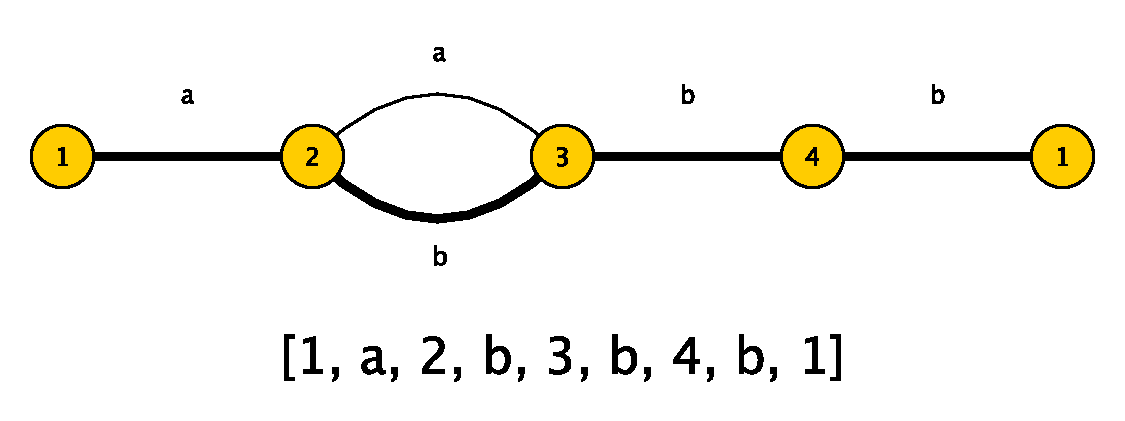
\includegraphics[width=0.5\textwidth]{images/Fig31.pdf}\\
	\caption{One of the possible way of traversing nodes for generating an ordered sequence of nodes' ids and time classes.}
	\label{fig:Fig31}
\end{figure}

\subsection{Global structural component}
\label{Global structural component}

The network embedding frameworks suffer from exploiting random or semi-random walk models as the main sampling strategy. Basically, it captures mostly proximity of nodes in a graph rather than the structural similarity of their neighbourhoods~\ref{Limitations of Node2vec}. Imputation of the global structural component is meant to overcome this shortcoming. It was inspired by the baseline idea of Role2vec framework~\cite{role2vec} which defines structural similarity by the node's membership to a certain structural class. Its authors Nesreen K. Ahmed et al. initially defined a set of structural classes and then assigned them to nodes based on their local structures regardless of their proximity in the graph. On the contrary, Node2vec structural similarity notion relies on the assumption that similar nodes are surrounded by similar context~\cite{role2vec}, means they have intersecting neighbourhoods.

The global node-based structural component can identify nodes playing similar structural roles (e.g. hub, bridge) in the different graph components and insert it to the ordered sequence of nodes' ids. ~\autoref{fig:Fig32} depicts a graph. Although red nodes belong to different components of the graph and are connected by the relatively long shortest path, they perform the same role of a local hub. Red nodes have relatively high degrees in the graph what makes them structurally similar to each other and different to other nodes in the graph.
\begin{figure}[!ht]
	\centering
	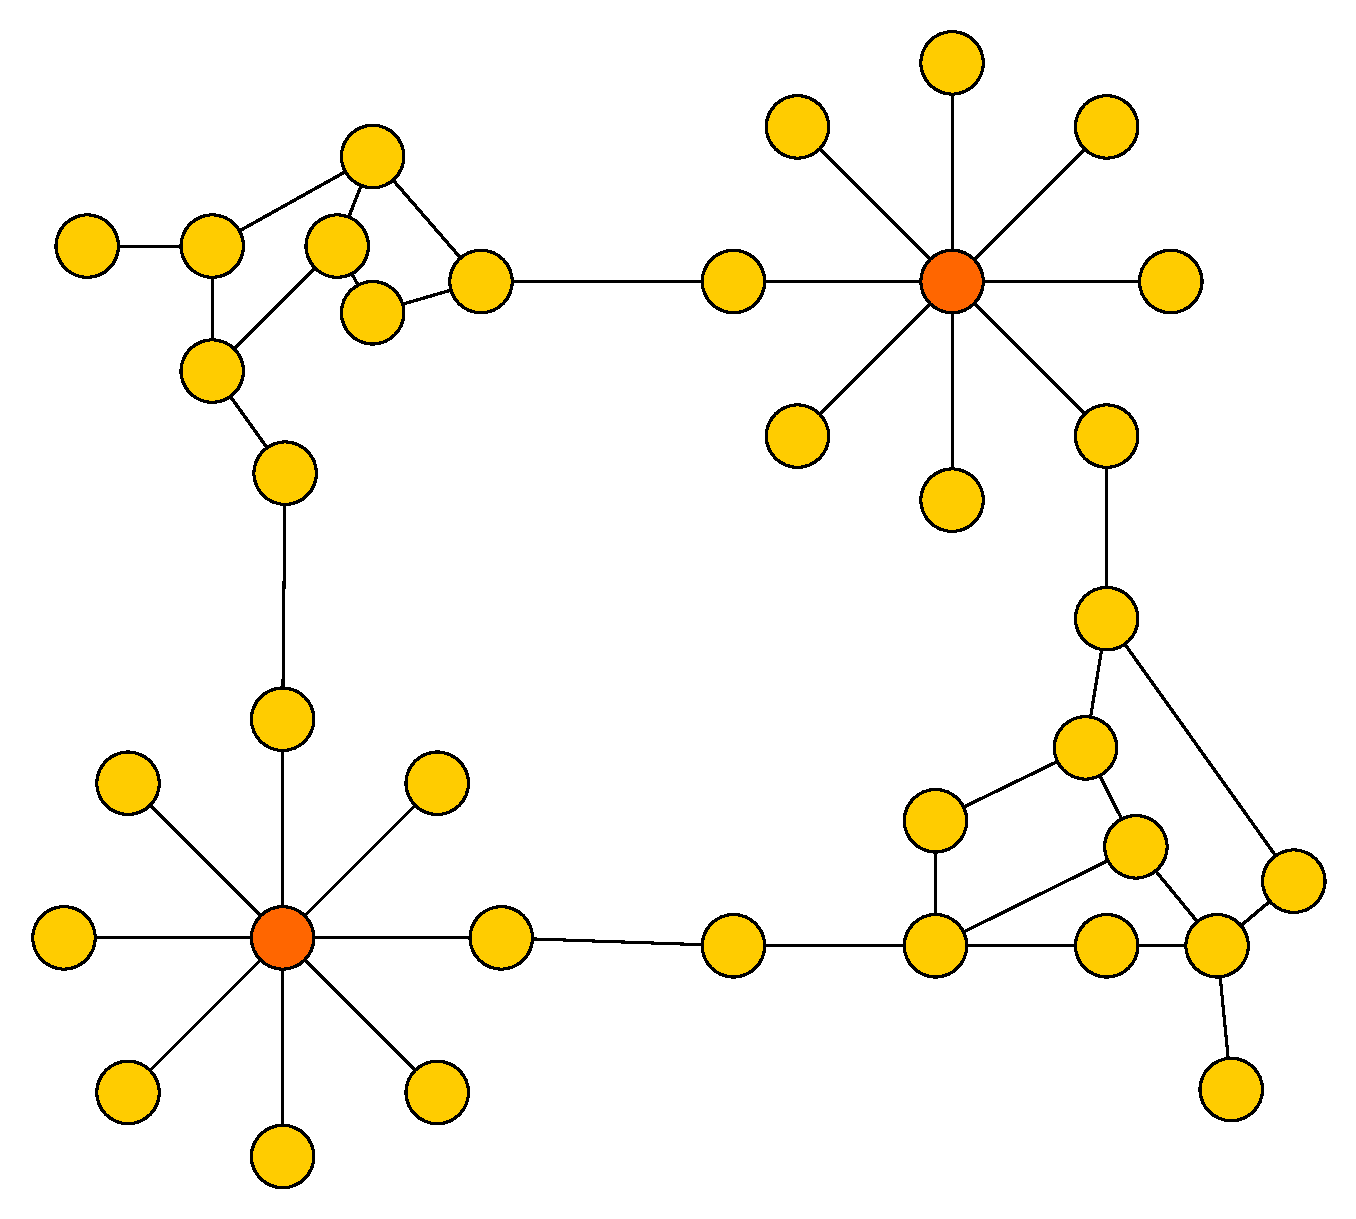
\includegraphics[width=0.3\textwidth]{images/Fig32.pdf}\\
	\caption{Red nodes belong to different components of the graph, whilst they are structurally similar and serve as local hubs.}
	\label{fig:Fig32}
\end{figure}

The imputation of the degree classes is similar to time classes imputation. The final sequences are the alternation of nodes' ids, acquired by the original Node2vec sampling and their degrees.

\section{Concept evaluation}
\label{Concept evaluation}
The overall concept is assessed by the goodness of the resulting clusters obtained from the final stage of the pipeline. Clustering results, in turn, are evaluated by a set of objective and quantitative measures. The majority of internal clustering evaluation measures are based on the intuition that clustering leads to the high similarity of the nodes within a cluster and low similarity between clusters. However, it is worth to mention that good scores on internal measures do not necessarily guarantee effective information retrieval from the original data.

~\autoref{tab:tab2} summarizes clustering evaluation indices used in the work. The list of metrics was inspired by~\cite{liu2010understanding} and~\cite{kovacs2005cluster}, their meanings along with calculation methods were explained in~\ref{Cluster evaluation strategies}.

\begin{table}[H]
\begin{center}
\begin{tabular}{ | m{0.7em} | m{8cm}| m{1.5cm} | m{2.6cm} |} 
\hline
\textbf{\#} & \textbf{validity measure} & \textbf{notation} & \textbf{optimal value} \\ 
\hline
1 & Root-mean-square standard deviation index & \textit{RMSSTD} & min \\ 
\hline
2 & R-square index & \textit{RS} & max \\ 
\hline
3 & SD Validity index  & \textit{SD} & min \\ 
\hline
4 & S\_Dbw Validity index   & \textit{S\_Dbw} & min \\ 
\hline
5 & Silhouette coefficient & \textit{SC} & max \\ 
\hline
6 & Davies–Bouldin index & \textit{DB} & min \\
\hline
7 & Dunn index & \textit{D} &  max \\
\hline
8 & Calinski-Harabasz index & \textit{CH} &  max \\
\hline
\end{tabular}
\caption {Internal clustering validation measures}
\label{tab:tab2}
\end{center}
\end {table}

These particular clustering evaluation measures are used for two main purposes.
\begin{enumerate}
  \item Although clustering results are affected to a large extent by user-defined input hyperparameters, there is no conventional way of choosing such hyperparameters. The above evaluation measures facilitate the tuning of clustering hyperparameters. Cluster analysis runs several times for each value of slightly changing hyperparameter or combination of hyperparameters. Each run generates a set of evaluation measures values. A clustering and its hyperparameter with the best measures' values are considered as the best set of clusters and the optimal hyperparameter.
  \item The pipeline is constructed as a branching tree. At the last stage, it outputs several clustering results from different branches which contain different cluster analysis techniques. It is crucial to have a unified scale for comparison of such results. The internal clustering evaluation measures in~\autoref{tab:tab2} are used to compare results from the different pipeline's branches and to find the best cluster set.
\end{enumerate}

\section{Summary}
This chapter covered the aim of the concept and its form - data science pipeline. Additionally, to three stages of the pipeline, it provided insights into data preparation and evaluation procedures. The main part of the chapter was devoted to the unique way of sampling from networks in the automated feature learning process. The proposed strategy in~\ref{Automated Feature Learning Framework} benefits from nodes' local neighbourhoods, time, and global structural components all in one. It is meant to enrich the learning capabilities of the framework, which will reveal in cluster analysis at the final stage.

The upcoming chapter leads through implementation details and introduces some third-party frameworks exploited at different stages of the developed pipeline.



\chapter{Implementation}
\label{cha:implementation}

The previous chapter explained the central concept of the work. The current chapter covers technical implementation details and addresses the following questions:

\begin{itemize}
  \item development tools, environments, frameworks and a programming language used for implementation.
  \item The sequential stages of the data processing pipeline with the set of techniques and their implementation.
  \item The application for interactive data visualization in a low-dimensional space. The application wrappers around the data science pipeline.
  \item The evaluation of the results of the branched pipeline and its implementation.
  \item Deliverables of the thesis.
\end{itemize}

\section{Implementation environment and programming language}
The basic data science pipeline~\ref{Overall data science pipeline for user segmentation} as well as the demo application~\ref{Demo application} are written in Python 3.7. Python is an interpreted, high-level, general-purpose programming language. It is developed under OSI-approved open source license. Numerous Python community developed a variety of libraries for almost any purpose. The language is equally good for building web server applications and manipulations with raw data, analysis and visualization. These were the decisive factors for choosing this particular programming language for the implementation part of the current work. The auxiliary packages along with the purposes of use in the present work are listed in the~\autoref{tab:tab3}.

The proposed data science pipeline is developed and submitted as a set of Jupyter Notebooks. Jupyter Notebook is an open-source web application commonly used for scientific computing and data science. It is suitable for working with live code, equations, visualizations and explanatory text all in one. It was intentionally developed for data cleaning and transformation, numerical simulation, statistical modelling, machine learning and other data science specific purposes~\cite{Jupyter_Notebook}. Jupyter Notebook was developed as a part of the open-source Jupyter project for interactive computing across different programming languages. It released under the liberal terms of the modified BSD license~\footnote{
\textbf{BSD license} is a class of simple and liberal licenses for computer software with two main restrictions: (1) one should not claim that they wrote the software if they did not write it and (2) one should not sue the developer if the software does not function as expected or as desired. Source: http://www.linfo.org/bsdlicense.html}.

PyCharm is an open-source cross-platform integrated development environment which supports web development in Python. It has plenty of features for writing code such as code analysis, a graphical debugger, an integrated unit tester. PyCharm Community Edition is distributed under Apache 2 license~\footnote{\textbf{Apache license} is a permissive free software license written by the Apache Software Foundation. Source: http://www.apache.org/licenses/}.

\begin{table}
\begin{center}
\begin{tabular}{ | m{0.7em} | m{1.7cm} | m{1.5cm} | m{11cm} |} 
\hline
\textbf{\#} & \textbf{package} & \textbf{version} & \textbf{purpose of usage} \\ 
\hline
1 & pandas & 0.23.4 & Data preprocessing and manipulations with data frames \\
\hline
2 & numpy & 1.16.4 & Work with multi-dimensional vectors \\
\hline
3 & datetime & 3.7 & Dates converting, transactions' timestamps processing \\
\hline
4 & random & 3.7 & Incorporation of time classes into semi-random walks in case of multi-edges \\ 
\hline
5 & networkx & 2.2 & Graph representation of financial transaction networks \\
\hline
6 & itertools & 3.7 & Generation of modified sequences by merging semi-random walks and additional information components \\
\hline
7 & matplotlib & 3.1.1 & 2d visualisation \\
\hline
8 & mplot3d & 3.1.1 & 3d visualisation \\
\hline
9 & scikit-learn & 0.21.2 & Clustering validation metrics  \\
\hline
10 & jqmcvi & 1.0 & Dunn clustering validation metric  \\
\hline
10 & math & 3.7 & Mathematical operations (sqrt) \\
\hline
11 & scipy & 1.2.1 & Spatial distances in a metric space \\
\hline
\end{tabular}
\caption {Python packages used for the implementation of the data science pipeline and demo application (compatible with Python 3.7 version).}
\label{tab:tab3}
\end{center}
\end {table}

\section{Overall data science pipeline for user segmentation}
\label{Overall data science pipeline for user segmentation}
This section covers each phase of the technical implementation of the developed pipeline. All stages are developed as a Python script. The sequential stages conceptually have been described in the previous chapter on the~\autoref{fig:Fig28}. This section will discuss in detail how they are implemented including data preparation, processing and evaluation phases.

The data preparation in general case includes converting a financial transaction data to a data set of $N$ transactions each of them described by "Source" - a user who initiates a transaction, "Target" - a user who received a transaction and "Timestamp" - when the transaction has been transferred. The next crucial step is to convert "Timestamp" feature to the time classes. To come up with the relevant time classes splitting, it is necessary to follow two rules: 
\begin{enumerate}
    \item The number of time classes should not be too large. As the goal is to come with the clusters of similar users, a time class should span enough users who were active during a certain time period.
    \item The number of time classes should not be too low. If too many users would be active during the same period, they will be placed close to each other in a metric space making too large indistinguishable clusters of similar users. 
\end{enumerate}
To choose the optimal number of time classes, some forehand time analysis is required. It may need to convert "Timestamp" values to datetime format to explore transaction distribution over time. In general, the time classes splitting is an input data set-dependent procedure.

The data processing phase consists of network embedding learning, dimensionality reduction and cluster analysis stages (\autoref{fig:Fig28}). The stages are implemented consequently within one Python script. The script exploits several existing frameworks chained together. These frameworks along with their original sources are listed in the~\autoref{tab:tab4}. The Node2vec framework is used for generating semi-random walks from a network. Then the semi-random walks are transformed to ordered sequences according to imputation strategies from~\ref{Time component} and~\ref{Global structural component}. The Word2vec from the gensim.models package provides a fast realization of the skip-gram model which allows learning features from ordered sequences. The next stage takes the output of skip-gram model as an input for further dimensionality reduction. The UMAP, t-SNE, and PCA frameworks produces low-dimensional embeddings from arbitrary dimensional data. This step facilitates the future cluster analysis by reducing the negative effects of the "curse of dimensionality". The next stage groups the outputting embeddings into clusters. Two frameworks HDBSCAN and k-means serve this purpose and produce sets of users split into clusters.
\begin{table}
\begin{center}
\begin{tabular}{ | m{0.7em} | m{2cm} | m{3.7cm} | m{1.5cm}| m{7cm} |} 
\hline
\textbf{\#} & \textbf{framework} & \textbf{software package} & \textbf{version} & \textbf{source} \\ 
\hline
1 & Node2vec & node2vec & 0.2.1 & https://github.com/eliorc/node2vec \\
\hline
1 & Word2vec & gensim.models & 0.10.2 & https://github.com/eliorc/node2vec \\
\hline
2 & UMAP & umap~\cite{mcinnes2018umap-software} & 0.3.9 & https://github.com/lmcinnes/umap  \\
\hline
3 & t-SNE & sklearn.manifold & 0.21.2 & https://scikit-learn.org \\
\hline
4 & PCA & sklearn.decomposition & 0.21.2 & https://scikit-learn.org \\ 
\hline
5 & HDBSCAN & hdbscan~\cite{mcinnes2017hdbscan} & 0.8.22 & https://github.com/scikit-learn-contrib/hdbscan \\
\hline
6 & k-means & sklearn.cluster & 0.21.2 & https://scikit-learn.org \\
\hline
\end{tabular}
\caption {Python software frameworks used for the implementation of the processing stages of the data science pipeline.}
\label{tab:tab4}
\end{center}
\end {table}

\begin{figure}[!ht]
	\centering
	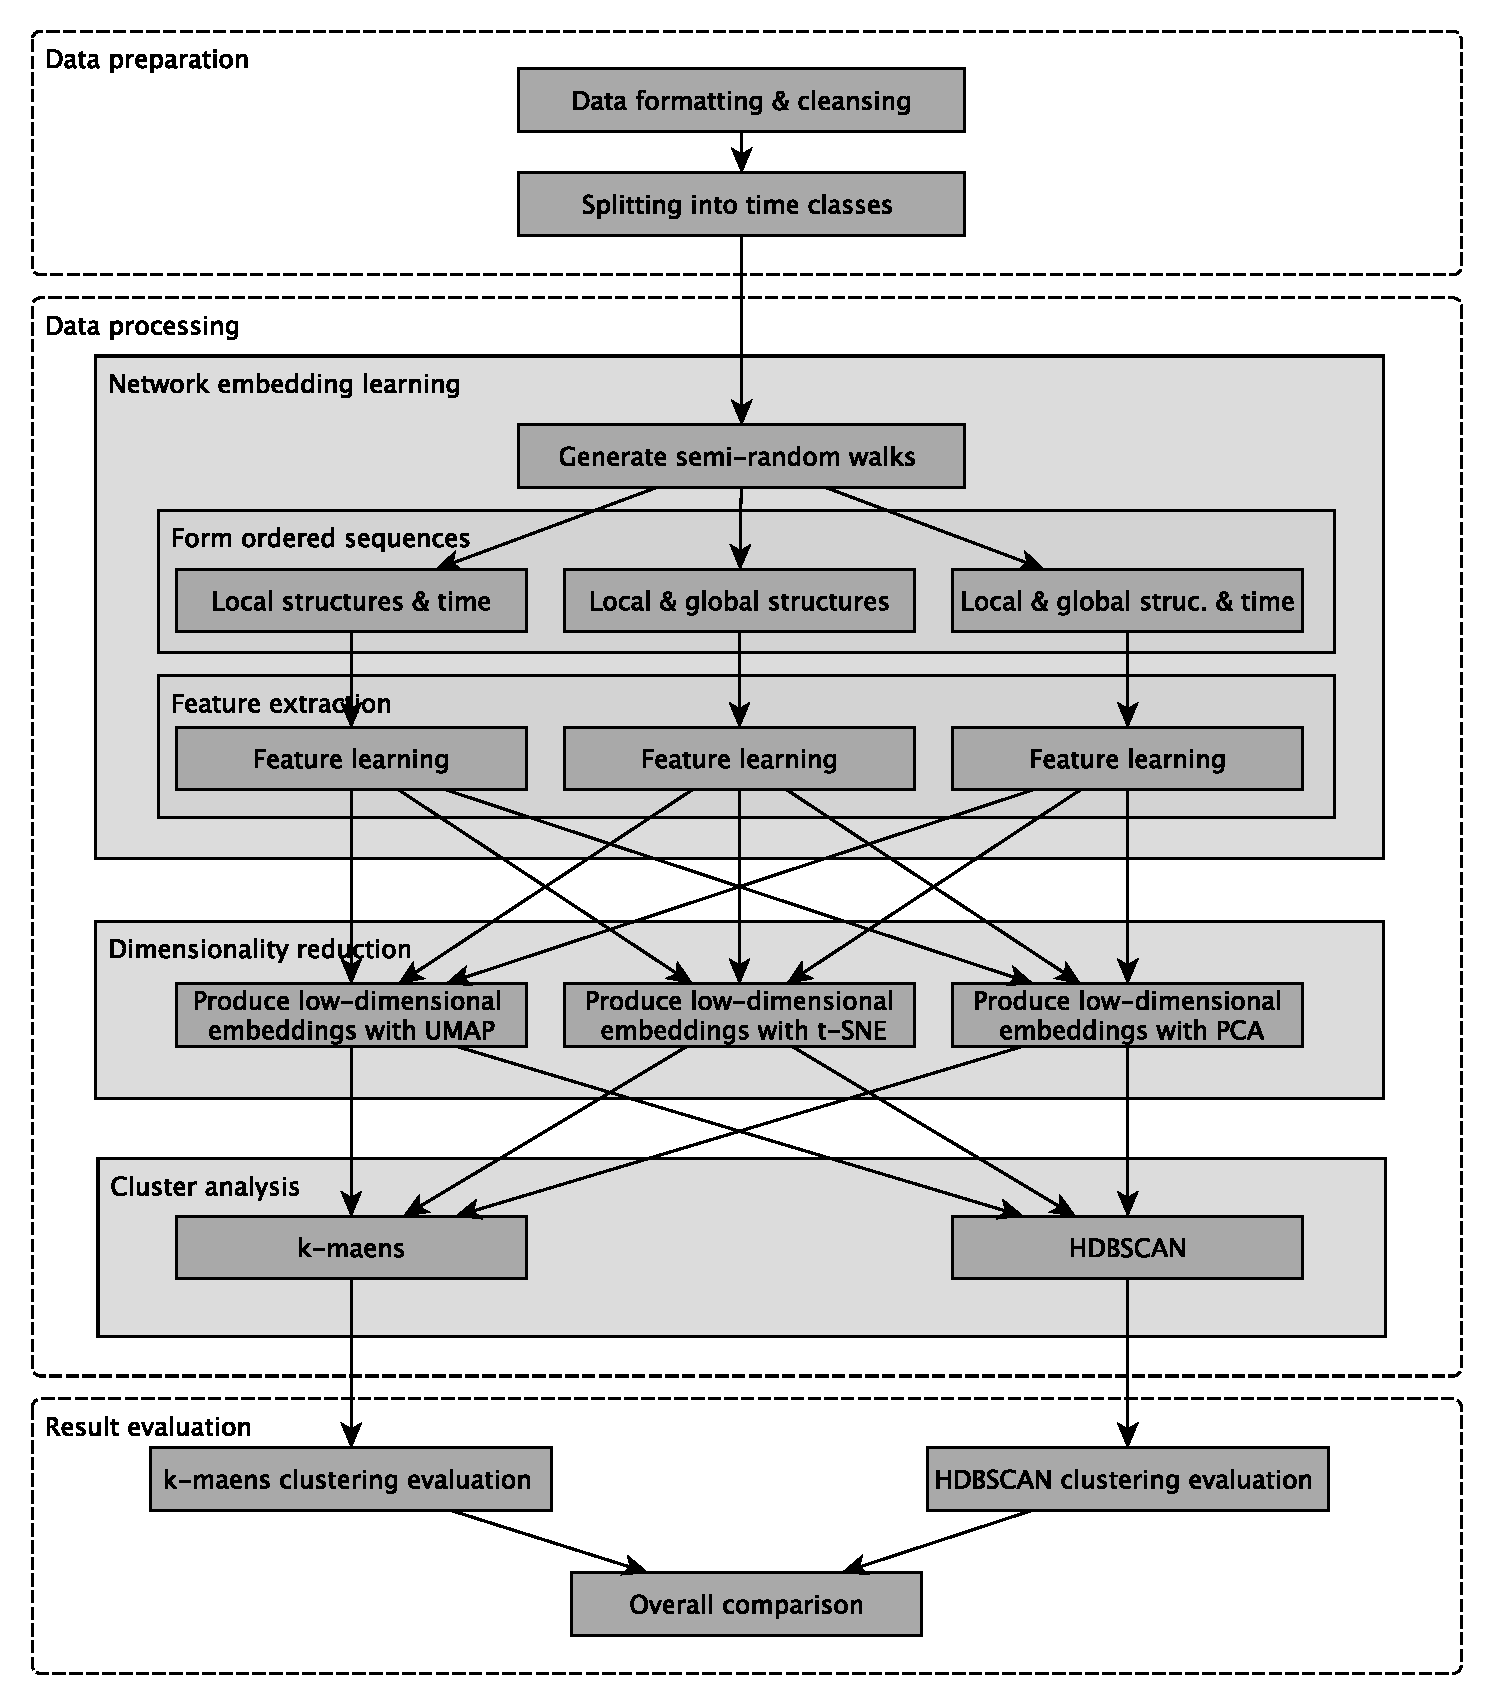
\includegraphics[width=0.67\textwidth]{images/Fig33.pdf}\\
	\caption{The implementation stages of the branched data science pipeline.}
	\label{fig:Fig33}
\end{figure}

The evaluation phase assesses the clustering quality by a set of internal validation measures~\footnote{\textbf{Internal clustering validation measures} - indices which are based on information from the data only and do not consider ground truth labels~\cite{hamalainen2017comparison}}. The set of 8 measures (discussed in~\ref{Concept evaluation}) helps to identify the best data partitioning in terms of compactness, connectedness and separation of clusters. First, the evaluation metrics are used to determine hyperparameters of a clustering, then to compare clustering results from all possible pipeline branches between each other. ~\autoref{fig:Fig33} presents the described overall pipeline divided into implementation stages. The arrows denote data flow along the all possible branches of the pipeline.

\section{Demo application}
\label{Demo application}
A web-based analytics application is developed to demonstrate the application of the concept to artificial data sets. It visualizes the resulting embeddings from the different pipeline's branches interactively. Furthermore, it allows to tune parameters of the unsupervised techniques used on different stages and to observe changes in the results immediately. 

The purpose is to demonstrate the idea by feeding the pipeline with the small artificial data sets, which are not only very fast to process but also exhibit extreme patterns of network structures. Due to these input examples, a user can quickly grasp the intuition behind the developed analytical approach. The set of artificially-generated inputs can be easily extended within the application. At the moment of the thesis delivery there are following predefined data sets:
    \begin{itemize}
        \item random network,
        \item star network,
        \item network of two disconnected star components,
        \item network of two connected star components,
        \item network of two disconnected components of nodes sampled from normal distributions,
        \item network of two disconnected components each sampled as a Watts–Strogatz model graph with edges belonged to 4 different time classes (2 classes per component),
        \item network of two disconnected components each sampled as a Watts–Strogatz model graph with edges belonged to 3 different time classes (1 class per component + 1 class presented in both components),
        \item grid graph model.
    \end{itemize}

From the technical perspective, the application is essentially a web-wrapper around the primary pipeline. It was implemented using Python framework - Dash. Dash is an abstraction built on top of Flask~\footnote{\textbf{Flask} is one of the most popular lightweight Python WSGI application frameworks based on the Jinja template engine and the Werkzeug WSGI toolkit. Source: https://flask.palletsprojects.com} which allows to wrap a user web-interface around a Python analytics script.~\autoref{fig:Fig34} depicts an architecture of the Dash application.

\begin{figure}[!ht]
	\centering
	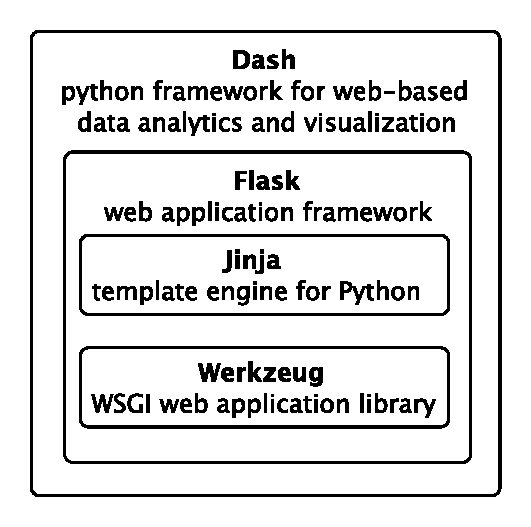
\includegraphics[width=0.35\textwidth]{images/Fig34.pdf}\\
	\caption{Architecture of the Dash application.}
	\label{fig:Fig34}
\end{figure}

The application provides an interactive user-friendly web-interface.~\autoref{fig:Fig35} presents the first screen of the interactive interface. A user can choose the initial parameters of Node2vec framework for feature learning from a selected network. Additionally, user chooses the components for ordered sequences generation (degree and/or time). The location component is chosen by default as it is necessary for Node2vec framework. The application visualizes the reduced embeddings in a 3d space produced by the three dimensionality reduction techniques. It also allows to set hyperparameters for these techniques and observe changes in the outputting visualizations.

\begin{figure}[!ht]
	\centering
	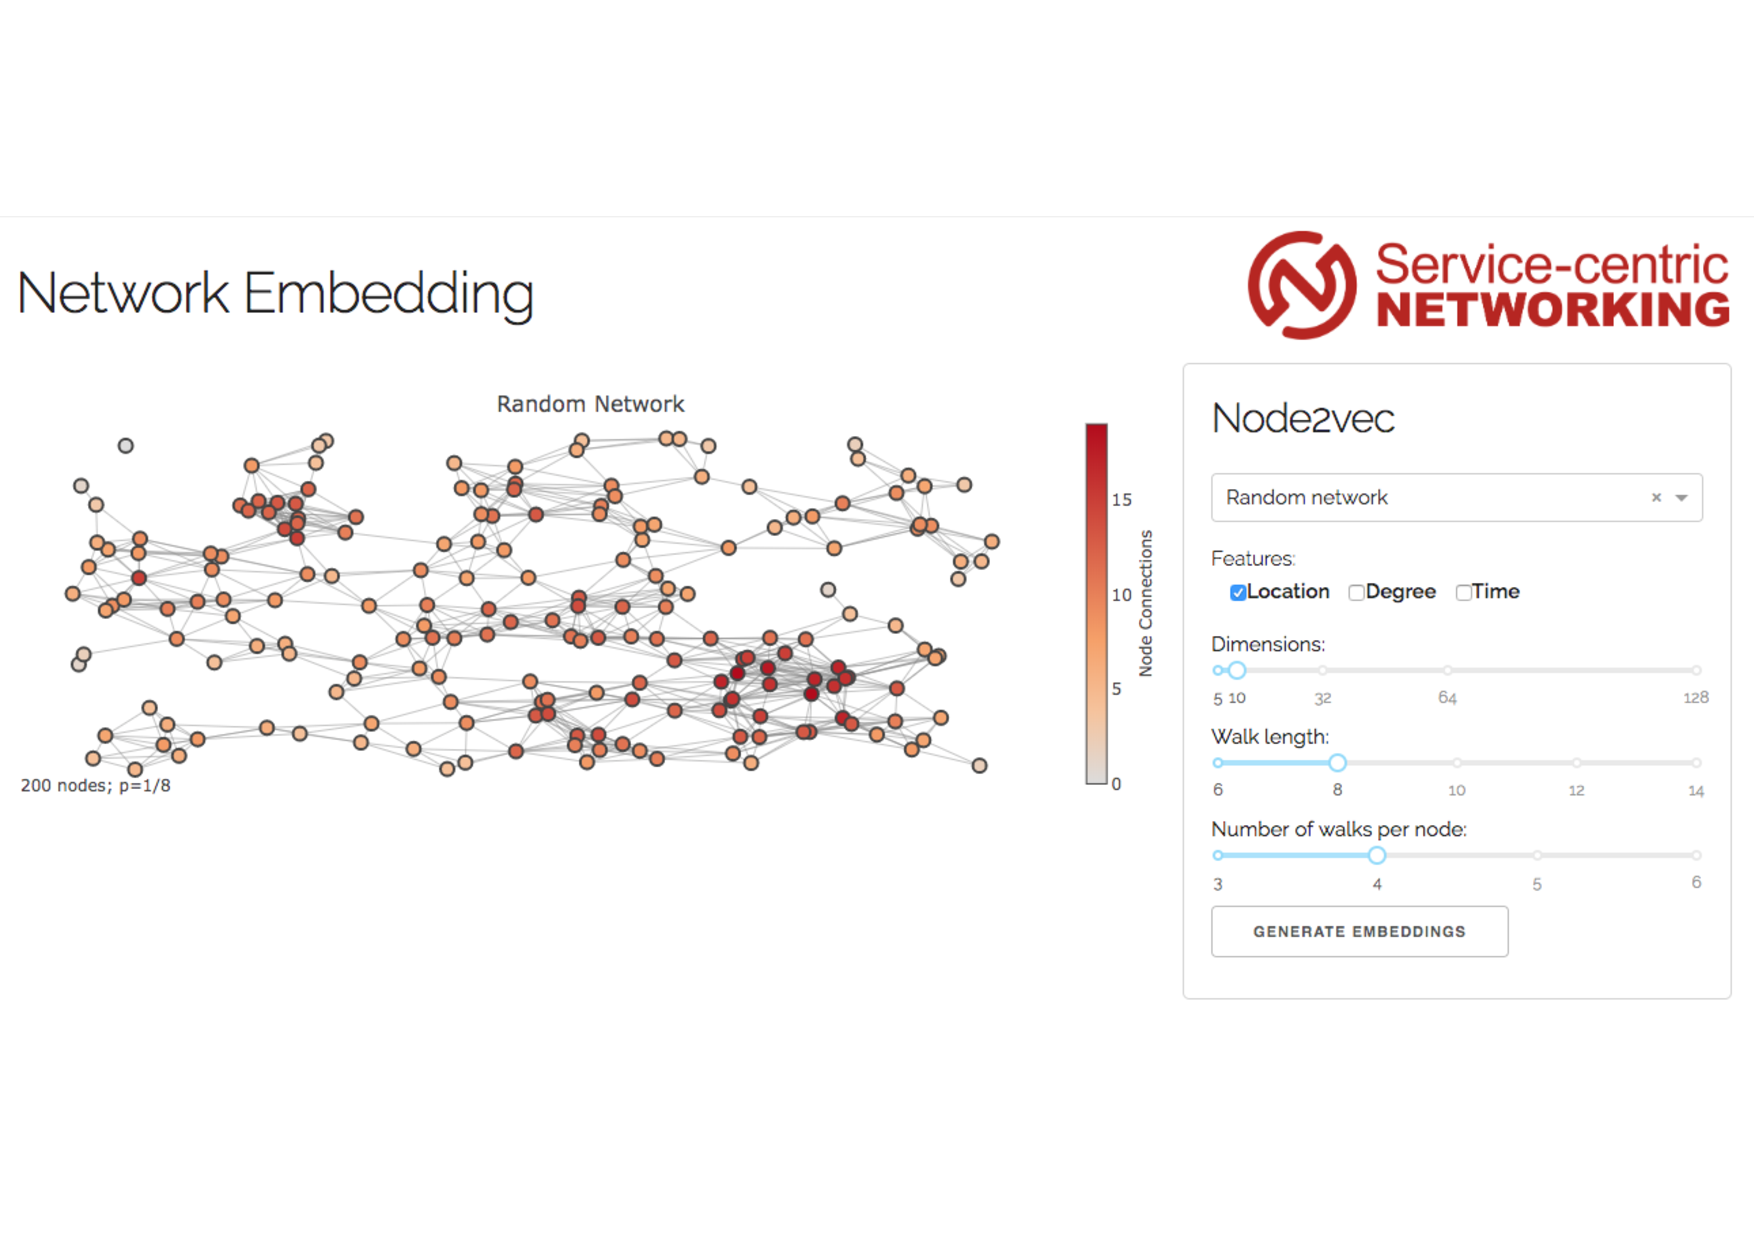
\includegraphics[width=0.65\textwidth]{images/Fig35.pdf}\\
	\caption{First screen web-interface of the application.}
	\label{fig:Fig35}
\end{figure}

\section{Result evaluation}
\label{Result evaluation}

The last stage of the pipeline produces a set of clusters. Thereby the evaluation of the concept boils down to measuring the quality of clustering.

As mentioned in~\ref{Cluster Analysis} there are various clustering techniques for different purposes and types of tasks. The pipeline exploits two very different from each other techniques on the same input data: partitional and density-based clustering. The goodness of clustering is typically measured by internal and external measures. While external validation metrics require ground truth labels, which in the current case is not provided, internal clustering validation metrics consider solely the available outputting clusters.

The evaluation stage of the obtained results on~\autoref{fig:Fig33} exploits a set of internal clustering validation metrics (listed in~\ref{Concept evaluation}). The achieved results from two different clustering techniques are compared separately. It means that outputs of several branches ended in $k$-means clustering will be compared among themselves. The comparison by eight internal validation metrics will highlight the leader among all possible k-means clustering results from the corresponding branches. However, k-means clustering has a well-known weakness in determining the number of clusters. The elbow method resolves this uncertainty by finding the best number of clusters for each particular branch result. The x-axis of the elbow plot described in~\ref{k-means} represents the number of clusters while the y-axis identifies the corresponding within-cluster sum of squares. The "elbow criterion" states to choose the number of clusters at which marginal gain in the within-cluster sum of squares drops and the curve outlines a slight angle. However, it is not always possible to clearly state the number of clusters $k$ from the plot. The set of internal clustering validation metrics facilitates the choice by pointing to a clustering with the best metrics' scores. Once the optimal number of clusters $k$ has been determined, the $k$-means clustering results from two branches compete with each other by achieving the best magnitudes for the eight internal clustering measures.

The second endpoint of the data processing stage on~\autoref{fig:Fig33} is the HDBSCAN clustering. This technique defines a number of clusters automatically by some density-based hiperparameters. A search grid helps to identify the best clustering parameters for each case. The grid considers the most crucial HDBSCAN clustering parameters:
    \begin{itemize}
        \item \textbf{minimum cluster size} - the minimum number of points recognized as a separate cluster,
        \item \textbf{minimum number of samples} - the number of samples in a neighbourhood for a point to be considered a core point (explained on the ~\autoref{fig:Fig23}),
        \item \textbf{alpha} - a distance scaling parameter (increasing alpha will make the clustering more conservative).
    \end{itemize}
Each HDBSCAN clustering result is generated for a different set of hyperparameters, estimated by the set of internal clustering measures, and then compared with other HDBSCAN results.

Finally, the two clustering winning results (one from k-means, one form HDBSCAN) are compared to each other in order to find the best clustering for the original input data.

\section{Deliverables}
The current work comes with the reproducible code of the implementation of the data science pipeline over the concept proposed in chapter~\ref{cha:conceptanddesign}. Additionally, the original financial data set used for the experiments described in the next chapter is attached.

This master thesis is submitted with a storage medium contained the following deliverables:
\begin{enumerate}
    \item Set of Jupyter notebooks written in Python: all data processing stages of the pipeline are implemented in Python 3.7. The notebooks contain all consecutive stages with comments, outputs, and related visualizations. They differ in the components considered for in the automated feature learning framework from networks at the first stage of the pipeline (described in~\ref{Automated Feature Learning Framework}):
    \begin{itemize}
        \item \textbf{Pipeline\_time.ipynb} contains all steps of the pipeline and considers the transactions' time of occurrence in the feature learning process \ref{Time component}.
        \item \textbf{Pipeline\_structures.ipynb} contains all steps of the pipeline and takes into account the global structural component described in the \label{Global structural component} in the feature learning.
        \item \textbf{Pipeline\_time\_structures.ipynb} contains all steps of the pipeline and considers both transactions' time and global structural component derived from a network.
    \end{itemize}
    \item Intermediate computational results of the experiments on the real-world data set:
    \begin{itemize}
        \item \textbf{Embeddings} - set of three files with the embeddings generated from the financial network by the automated feature learning framework (each file for time, global structures, and time-global structures components used for embeddings learning).
        \item \textbf{Labels} - set of three files with arrays of labels: the ids of the nodes whose representations have been learned.
        \item \textbf{K-means clustering results} - set of files with clusters of nodes grouped together as similar in some sense. They result from the branched pipeline using $k$-means clustering.
        \item \textbf{HDBSCAN clustering results} - set of files with clusters of nodes grouped together as similar in some sense. They result from the branched pipeline using HDBSCAN clustering.
    \end{itemize}
    \item Real-world data set of financial transactions between users of the~\href{www.prosper.com} platform. The data set consists of "Source" and "Target" fields which denote the users with the valid prosper account on the platform and "Timestamp" characterising when a "Source" has initiated a transaction to a "Target".
    \item Web-based analytics demo application highlights the main pipeline stages and interactively illustrates the idea by processing artificially-generated basic examples. It allows to tune model's hyperparameters and produces 3d visualizations.
\end{enumerate}

\section{Summary}
This chapter discussed the toolset involved in the development and justified its choice. Here, a reader can find the list of frameworks and packages along with their purposes of usage in the current work. The implementation of the pipeline's stages was discussed in detail. The chapter demonstrated the data flow along the pipeline branches and described the expected result. Additionally, the technical aspects of the demo application were outlined. The chapter explained the evaluation strategy exposed to the achieved results and listed the thesis deliverables.

\chapter{Experiments and evaluation}
\label{cha:evaluation}

This chapter presents the evaluation of the developed data science pipeline for unsupervised user segmentation in financial transaction networks over the real-world data set in different scenarios. It comprises the following:
    \begin{itemize}
        \item description of the data set used for experiments,
        \item description of the experimental conditions, computing environment and intermediate results,
        \item validation of $k$-means and HDBSCAN clustering results,
        \item overall comparison of the results,
        \item interpretation of the output.
    \end{itemize}

\section{Real-world data set}
In spite of the deficiency of publicly available financial transaction data sets, yet some of them are available for research. One of the leading platforms generating financial data - Prosper.com~\cite{Prosper}. It is a financial peer-to-peer lending platform, where individuals can either invest in personal loans or request to borrow money. Since its inception in 2005, the platform's cumulative lending volume has reached \$7 billion by 2015. To convince investors of the reliability of a borrower, Prosper.com discloses performance statistics, market data and loan histories on its website. This data can be represented as a financial transaction network, where nodes are lenders and borrowers, edges are issued loans (transactions).

The original network data set~\cite{konect:2017:prosper-loans} consists of 89.269 unique nodes, 3.394.979 edges and spans a period from November 15th, 2005 until September 27th, 2011. The proposed pipeline takes as an input transactions occurred between November 15th, 2005 and December 1st, 2006. Transactions have "Source", "Target", and "Timestamp" features, which result in 5.8 MB of input data. The original data set was cut off in order to be able to visualize produced embeddings in a low-dimensional space.

Some characteristics of the input network data:
\begin{itemize}
    \item it allows multiple edges but not loops,
    \item nodes' degree distribution follows the Power law
    \item network exhibits the properties of a small-world network~\footnote{\textbf{Small-World properties} - a high  clustering coefficient and a small characteristic path length of a network~\cite{Mehlhorn2013}.}
\end{itemize}

\section{Experimental conditions and computing environment}

All computational experiments performed on the server operating system Ubuntu 16.04.6 with 8 GB RAM. The code is written in Python 3.7.3, run inside the Jupyter notebook version 4.4.0 with iPython version 7.4.0. 

The intermediate results, specifically sets of generated embeddings are written to the disk as comma-separated files and can be reused for any other analysis.

\section{Evaluation of clustering results}

This section presents $k$-means and HDBSCAN clustering results. The internal clustering metrics are used for clustering validation in order to define the optimal hyperparameters, for evaluation and comparison of the results.

The developed data science pipeline operates for the three main combinations of components in the ordered sequence discussed in~\ref{Automated Feature Learning Framework}. As local structural component is necessary for Node2vec learning framework, the possible combinations of the components for feature learning from networks look as follows: 
    \begin{enumerate}
        \item local structural and time components
        \item local and global structural components
        \item local and global structural and time components
    \end{enumerate}
Every learned feature sets is being reduced in dimensions by UMAP, t-SNE, PCA and clustered by $k$-means and DBSCAN afterwards. 

\subsection{$k$-means clustering}

This section takes a close look at the evaluation and comparison of the particular branches' results: \textit{local and global structural components learning -> dimensionality reduction -> $k$-means clustering}. For the other branches' results evaluation see the appendices 1-2.

\subsubsection{Determining the number of clusters}
~\autoref{fig:Fig37} visualizes the embeddings in 3d space after the network feature learning (local and global structural components) and dimensionality reduction stages of the pipeline. Here the global structural component was defined by degree classes. In total 12 classes were distinguished each of them counts roughly 1000 nodes. The classes implicitly denote nodes' structural importance within the network through their degree: 1-degree nodes belong to the first class, 2 and 3-degree nodes to the second class, and so forth. The last 12th class is assigned to the nodes of the highest degrees (over 90). They are the most structurally important hubs in the network.
% \iffalse
\begin{figure}[!ht]
	\centering
	\includegraphics[width=1.0\textwidth]{images/evaluations/Fig37.pdf}\\
	\caption{Embeddings sets reduced to 3 dimensions by three dimensionality reduction techniques.}
	\label{fig:Fig37}
\end{figure}
\begin{figure}[!ht]
	\centering
	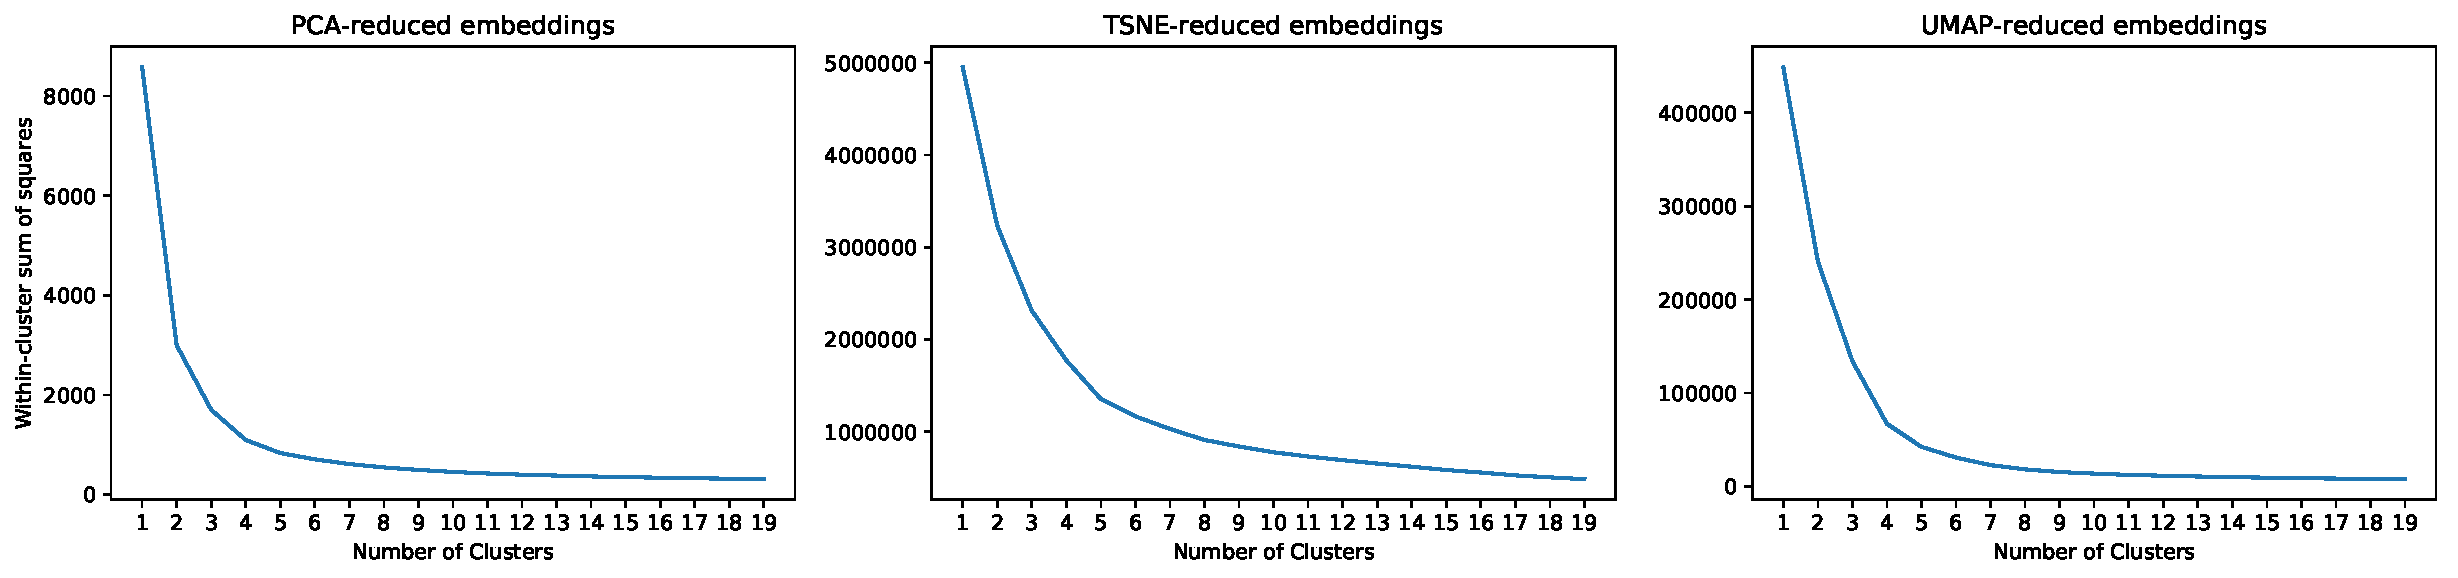
\includegraphics[width=1.0\textwidth]{images/evaluations/Fig38.pdf}\\
	\caption{Elbow plots for reduced embeddings sets.}
	\label{fig:Fig38}
\end{figure}
\begin{figure}[!ht]
	\centering
	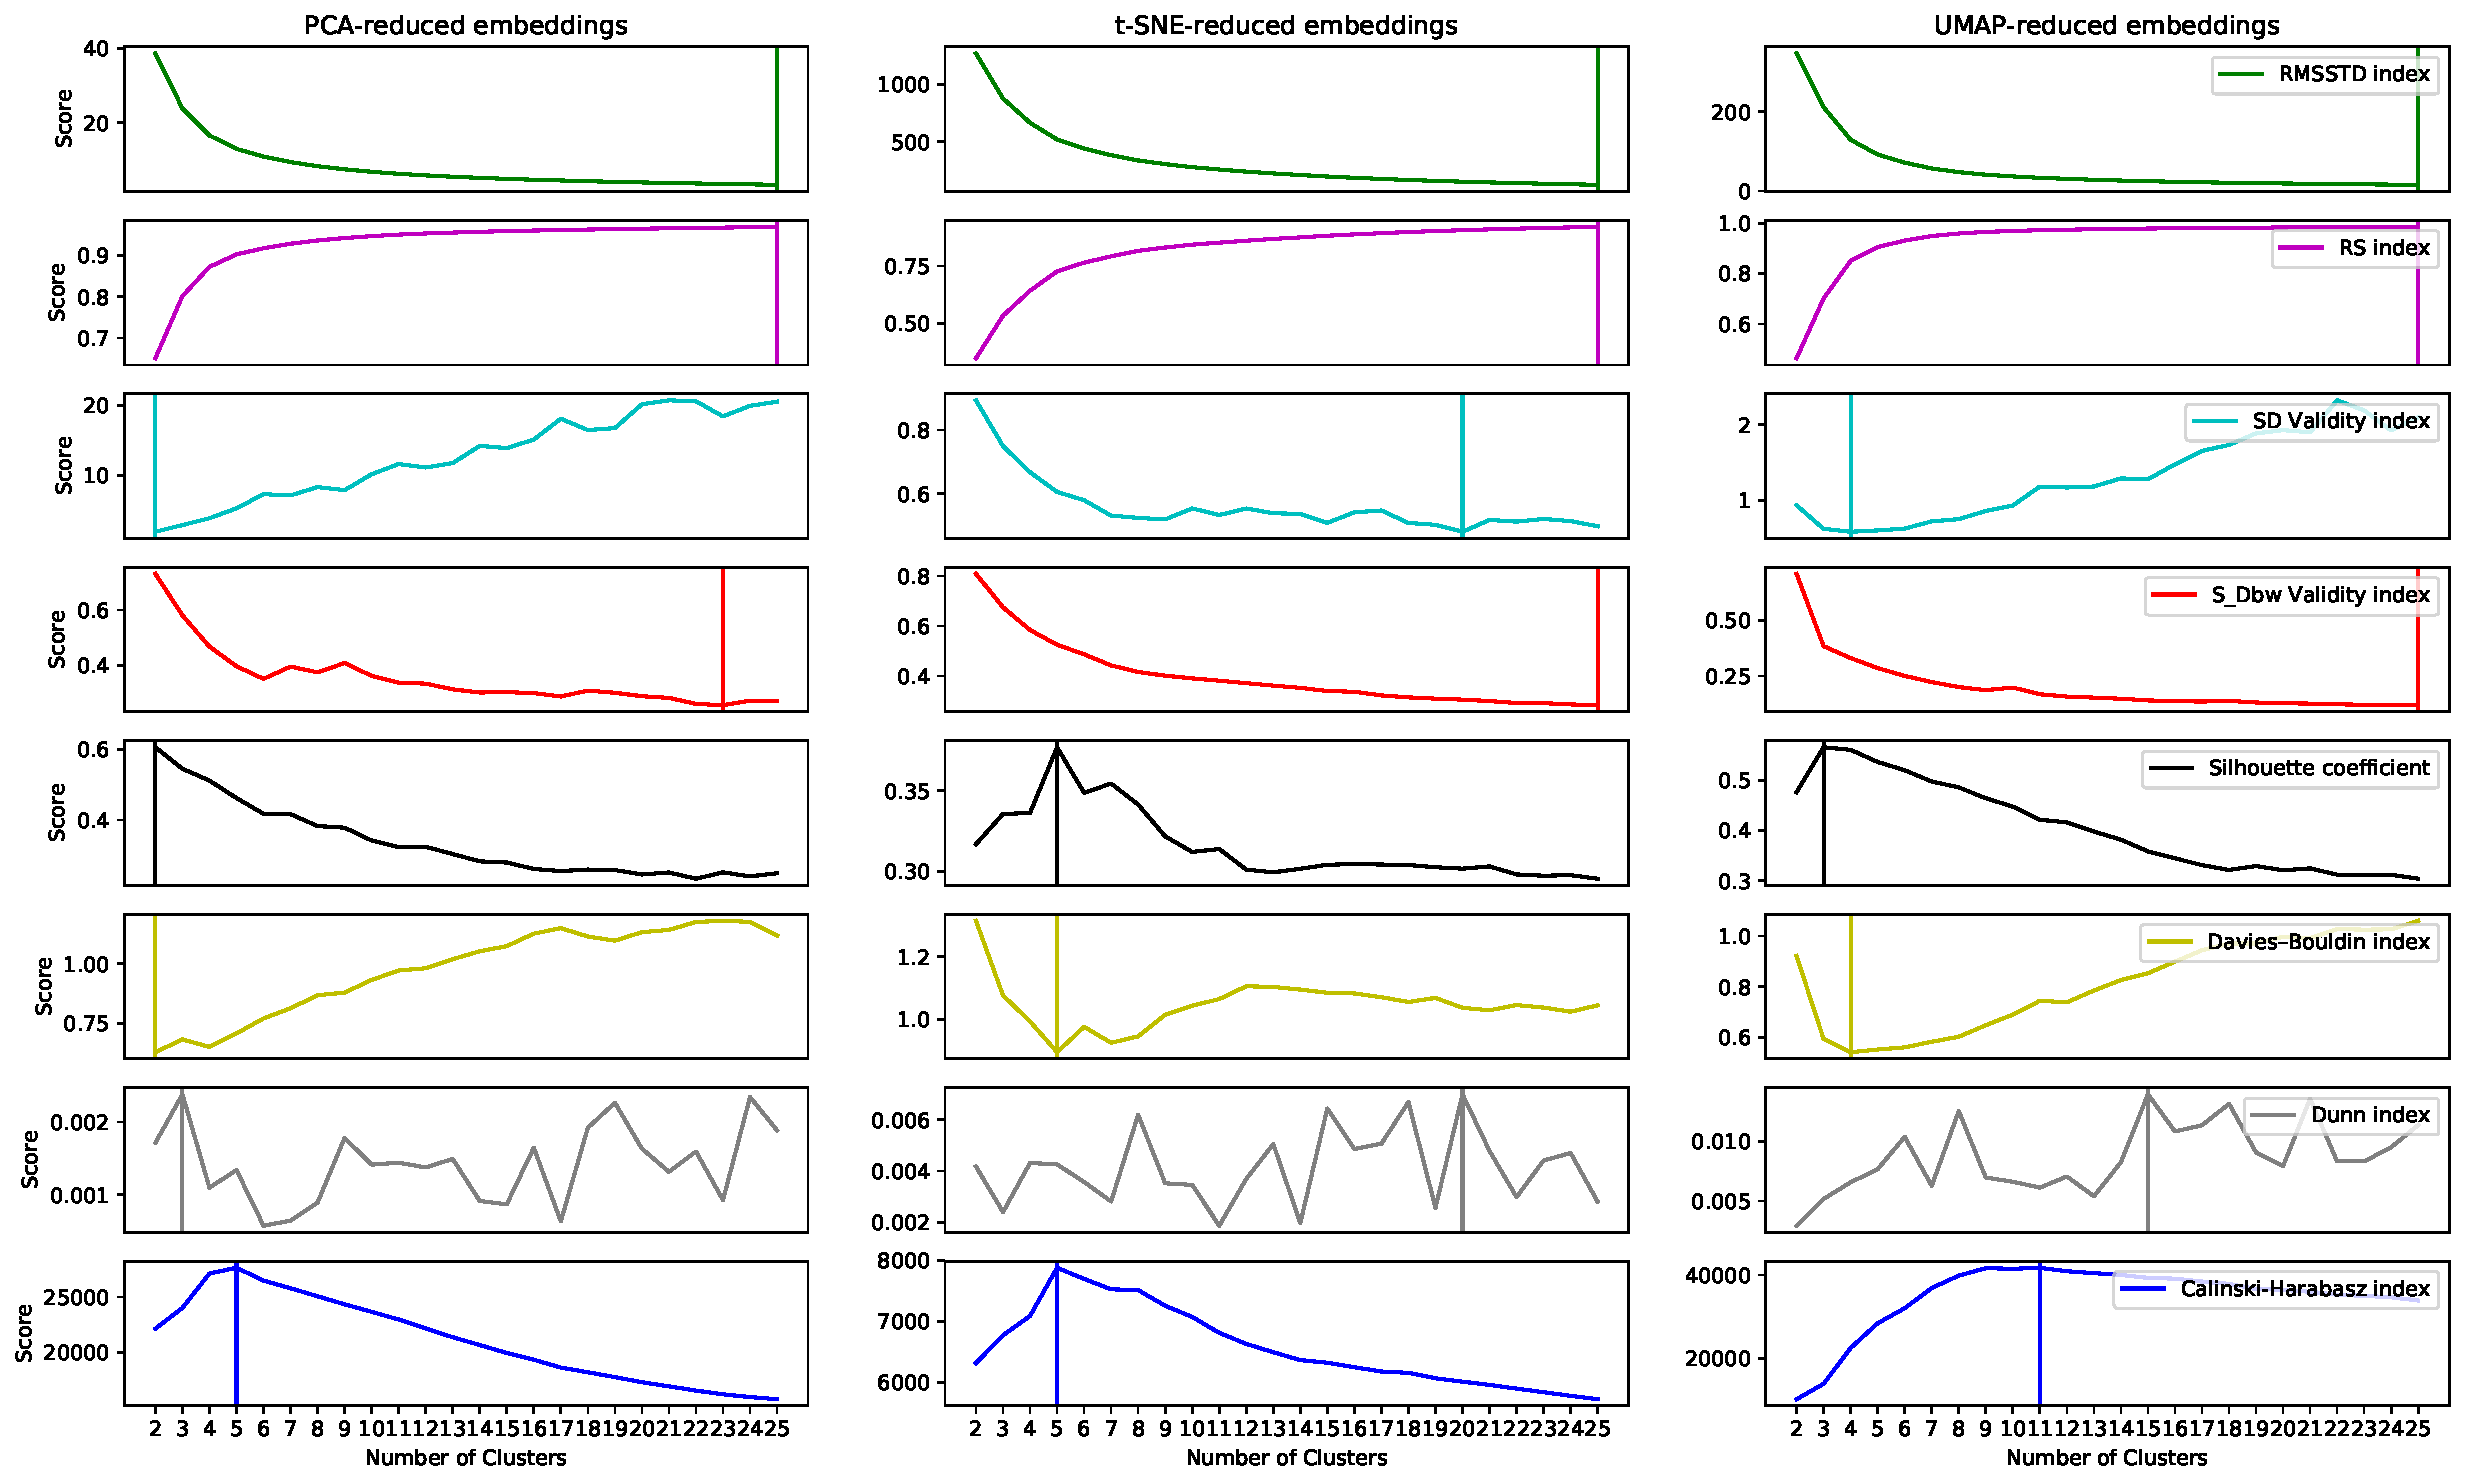
\includegraphics[width=1.0\textwidth]{images/evaluations/Fig39.pdf}\\
	\caption{Evaluation of $k$-means clustering with respect to the number of clusters $k$.}
	\label{fig:Fig39}
\end{figure}
% \fi

Elbow criterion facilitates the choice of an appropriate number of clusters for $k$-means. However, the elbow curves on the~\autoref{fig:Fig38} still leave some room to speculate about the right numbers of clusters: 3 or 4 clusters for PCA embeddings, 5 clusters for t-SNE, and 4 or 5 clusters for UMAP embeddings. To reduce that uncertainty it is helpful to compute the internal clustering measures for different numbers of $k$. ~\autoref{fig:Fig39} provides visualizations of measures' values varying with the increasing numbers of $k$ for every reduced embeddings set. The vertical lines at each plot denote the best choice of $k$ suggested by a particular measure (max or min).

The comprehensive analysis of the metrics from~\autoref{fig:Fig38} and ~\autoref{fig:Fig39} concludes the optimal $k$ equal to 4 for PCA-reduced embeddings, 5 for t-SNE-reduced embeddings, and 4 for UMAP-reduced embeddings. The intuition under this selection is exampled below for the t-SNE-reduced embeddings case:
\begin{enumerate}
    \item on the~\autoref{fig:Fig38} the marginal gain in within-cluster sum of squares drops significantly after the $k = 5$;
    \item on the~\autoref{fig:Fig39} RMSSTD, RS, and S\_Dbw Validity indices are generally higher if the number of clusters grows since they mostly aim at minimizing within-cluster inertia. They are not very meaningful in this case, unlike Silhouette coefficient, Davies–Bouldin, and Calinski-Harabasz indices, that suggest picking $k = 5$;
    \item although Dunn and SD Validity indices do not reach extremum at $k = 5$, they demonstrate slight convex and concave respectively at this point.
\end{enumerate}
The above intuition works for the rest cases for choosing $k$ in $k$-means clustering. ~\autoref{fig:Fig40} shows the resulting $k$-means clustering of initial sets from ~\autoref{fig:Fig37}. Refer to appendix 1-2 for the rest of the cases.  §
% \iffalse
\begin{figure}[!ht]
	\centering
	\includegraphics[width=1.0\textwidth]{images/evaluations/Fig40.pdf}\\
	\caption{Embeddings sets coloured by k-means clusters.}
	\label{fig:Fig40}
\end{figure}
% \fi
\subsubsection{Finding the best $k$-means clustering}
\label{Finding the best $k$-means clustering}
The previous section explains the choice of $k$ in $k$-means clustering. The current section compares clustering results among pipeline's branches ending by $k$-means.~\autoref{tab:tab5} collected the internal clustering metrics values rounded to the third digit (or other where appropriate) for each of nine $k$-means clusterings. The metrics were extensively discussed in the~\ref{Cluster evaluation strategies} along with their respective optima. The closest to optima values of measures are highlighted bold. The best values belong to $k$-means clustering of embeddings learned from the local and global structural components of the network and then reduced by UMAP. This clustering reaches the best or the second-best values in seven metrics out of eight. The visualization of the leading $k$-means clustering in a metric space is depicted on the~\autoref{fig:Fig40} right.

\begin{table}
\begin{center}
\small
\begin{tabular}{lrrrrrrrrrr}
\hline
\multicolumn{1}{l}{ } & \multicolumn{3}{c}{\textbf{loc + time}} & \multicolumn{3}{c}{\textbf{loc + glob}} & \multicolumn{3}{c}{\textbf{loc + time + glob}} \\
\cline{1-1} \cline{2-4} \cline{5-7} \cline{8-10} 
measure & PCA & t-SNE & UMAP & PCA & t-SNE & UMAP & PCA & t-SNE & UMAP & opt\\
\hline
RMSSTD & 44.14 & 791.7 & 158.4 & \textbf{16.53} & 520.4 & 129.5 & 33.60 & 602.8 & 89.72 & min \\
RS     & 0.530 & 0.569 & 0.658 & \textbf{0.873}  & 0.726   & 0.850  & 0.616 & 0.665 & 0.775 & max \\
SD     & 1.998 & 0.725 & 0.857 & 3.864  & 0.605   & \textbf{0.586}  & 2.814 & 0.666 & 1.003 & min \\
S\_Dbw & 0.962 & 0.657 & 0.592 & 0.467  & 0.525   & \textbf{0.330}  & 0.956 & 0.573 & 0.480 & min \\
SC     & 0.506 & 0.350 & 0.431 & 0.511  & 0.377   & \textbf{0.561}  & 0.465 & 0.354 & 0.371 & max \\
DB     & 0.988 & 1.006 & 0.847 & 0.651  & 0.897   & \textbf{0.541}  & 0.946 & 0.917 & 0.879 & min \\
D      & 0.0024 & 0.0025 & \textbf{0.006829} & 0.001  & 0.002 & 0.006567 & 0.0012 & 0.0054 & 0.0055 & max \\
CH     & 6969.6 & 7850.2 & 1449.4 & \textbf{27102.9} & 7880.5 & 22499.8 & 6352.8 & 7862.3 & 10184.8 & max \\
\hline
\end{tabular}
\caption {$k$-means clustering evaluation of the pipeline brunches ended in $k$-means}
\label{tab:tab5}
\end{center}
\end {table}

\subsection{HDBSCAN clustering}

The current section repeats the intuition from the above for determining an appropriate number of clusters and finding the best branch's result for HDBSCAN clustering. For the sake of consistency, the same branches' results will be examined, and evaluations of the rest branches' results are presented in the appendices 1-2.

\subsubsection{Determining the number of clusters}
Unlike $k$-means clustering where a number of clusters is a user-defined parameter, HDBSCAN clustering determines it automatically. However, HDBSCAN requires the set of input hyperparameters: \textit{minimum cluster size, minimum number of samples, alpha} (explained in~\ref{Result evaluation}). The best combination will be found automatically via a grid search algorithm. The three hyperparameters are varying between the certain appropriate ranges suggested by HDBSCAN creators in~\cite{mcinnes2017hdbscan}. HDBSCAN clustering is validated on 27 combinations of three hyperparameters by the set of six internal clustering measures (the initial eight measures from~\ref{Concept evaluation} except two working only for globular clusters - RMSSTD and RS indices). Similar to the $k$-means clustering evaluation, the best HDBSCAN clustering result is defined by the best measures magnitudes.

~\autoref{fig:Fig41} shows the varying values of the internal clustering metrics over different combinations of HDBSCAN hyperparameters for the embeddings learned from the local and global structural components of the network. In case of t-SNE-reduced embeddings set, the best choice of three hyperparameters are 20 for minimum cluster size, 5 for minimum number of samples, and 0.25 for alpha.~\autoref{fig:Fig42} visualizes the reduced embeddings from ~\autoref{fig:Fig37} coloured according to the HDBSCAN defined clusters (in this case 2 clusters in every set). Refer to the appendix 1-2 for HDBSCAN clustering evaluations of the other branches' results ending by HDBSCAN.

% \iffalse
\begin{figure}[!ht]
	\centering
	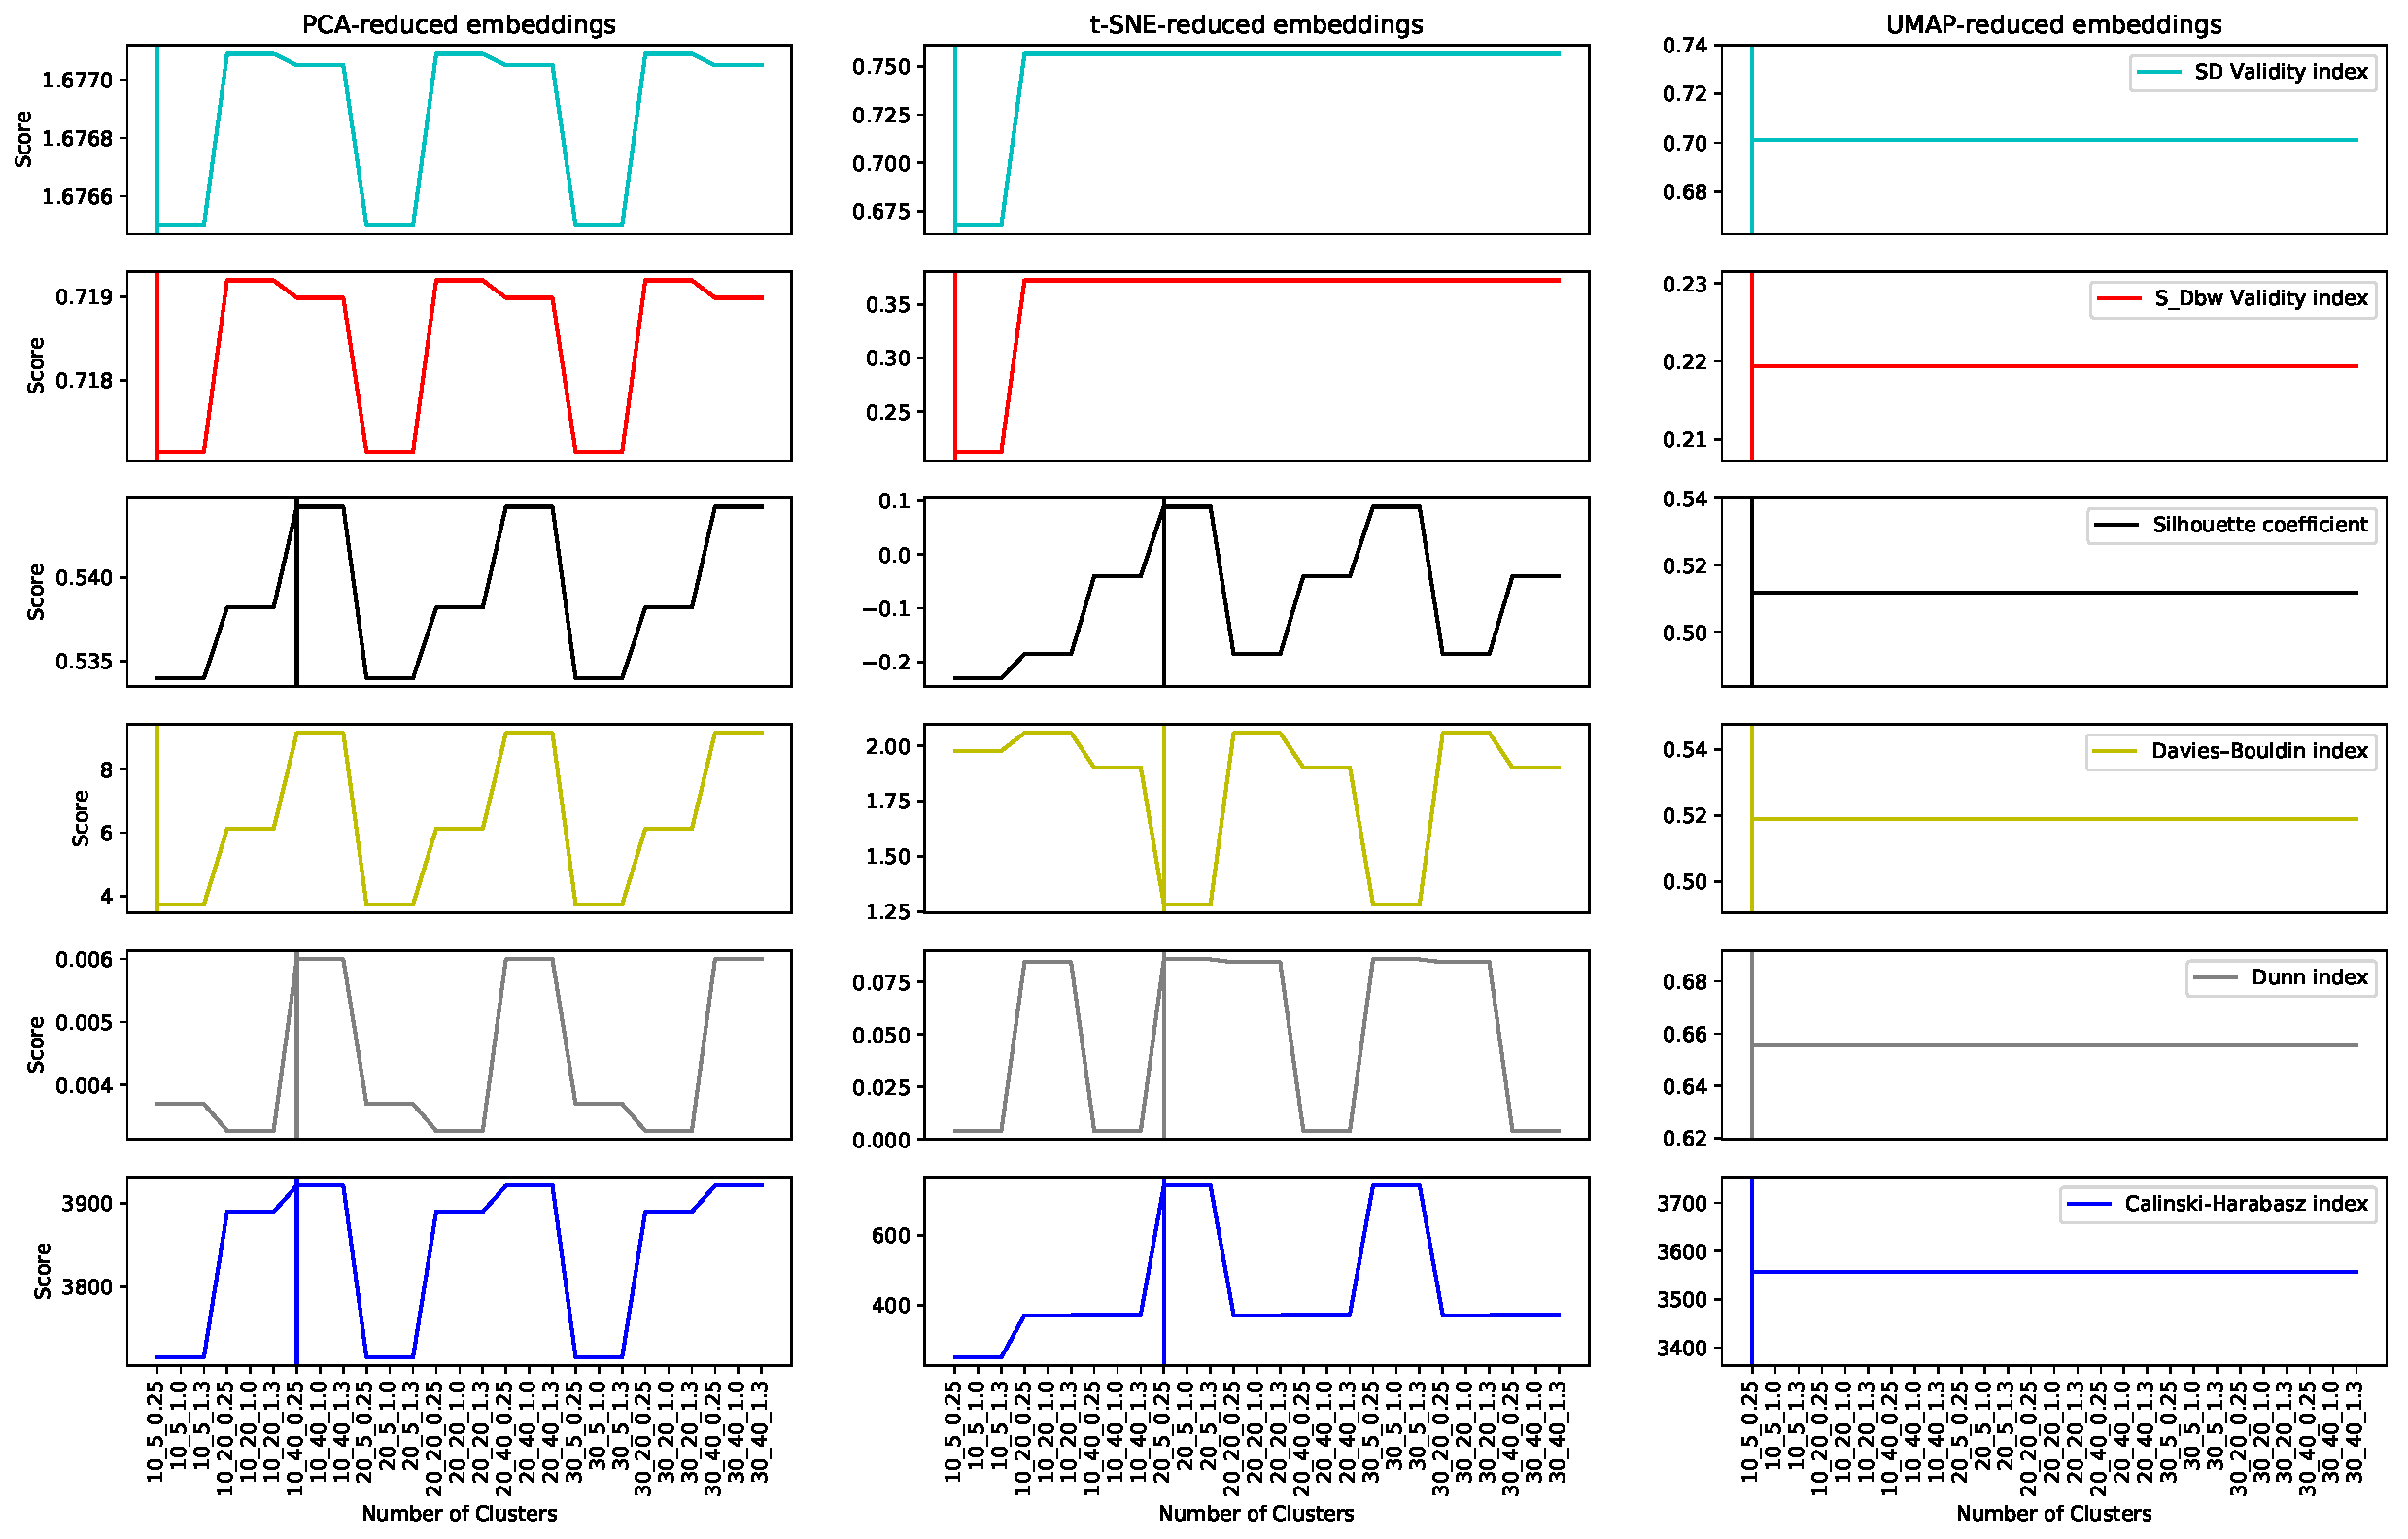
\includegraphics[width=1.0\textwidth]{images/evaluations/Fig41.pdf}\\
	\caption{Evaluation of HDBSCAN clustering with respect to the combination of hyperparameters (x axis: minimum cluster size\_minimum number of samples\_alpha).}
	\label{fig:Fig41}
\end{figure}
\begin{figure}[!ht]
	\centering
	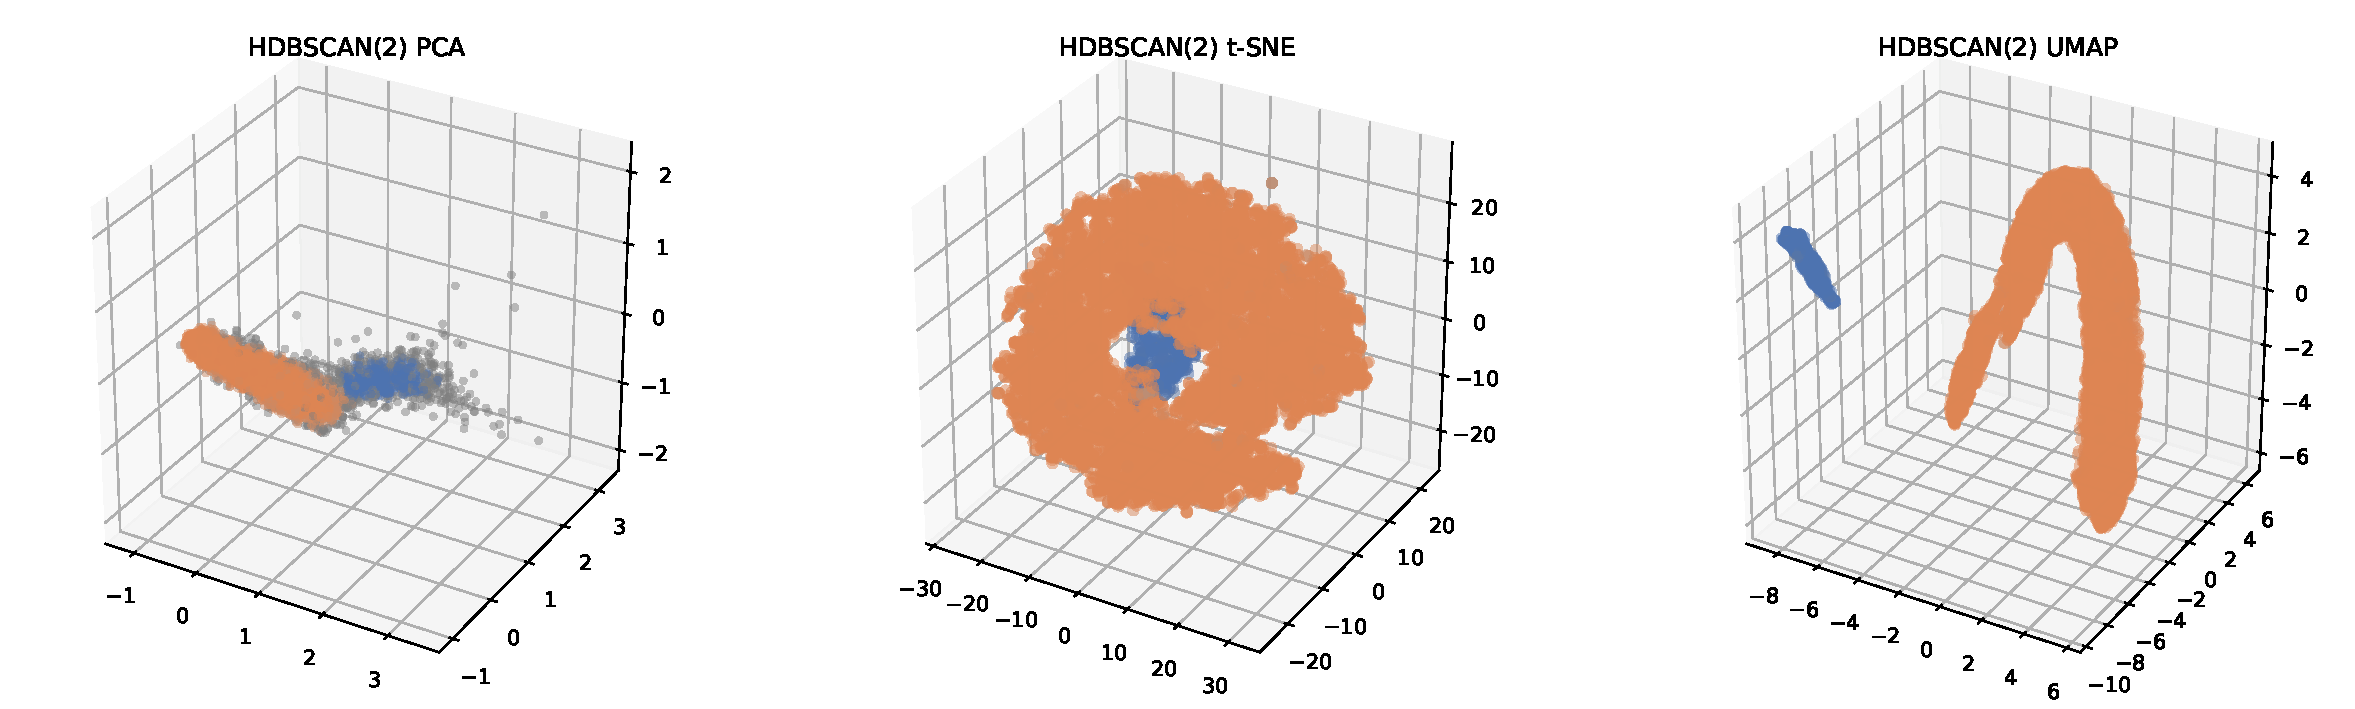
\includegraphics[width=1.0\textwidth]{images/evaluations/Fig42.pdf}\\
	\caption{Embeddings sets coloured by HDBSCAN clusters.}
	\label{fig:Fig42}
\end{figure}
% \fi

\subsubsection{Finding the best HDBSCAN clustering}
The best HDBSCAN clustering will be chosen from the nine possible reduced data sets.~\autoref{tab:tab6} presents the internal clustering metrics' values for HDBSCAN clustering. The best clustering is determined likewise~\ref{Finding the best $k$-means clustering}. In the current case, UMAP-reduced data set learned from the local and global structural components of the network is superior over others. It has the best values for two metrics (highlighted bold) and the second-best values for another two.

\begin{table}
\begin{center}
\small
\begin{tabular}{lrrrrrrrrrr}
\hline
\multicolumn{1}{l}{ } & \multicolumn{3}{c}{\textbf{loc + time}} & \multicolumn{3}{c}{\textbf{loc + glob}} & \multicolumn{3}{c}{\textbf{loc + time + glob}} \\
\cline{1-1} \cline{2-4} \cline{5-7} \cline{8-10} 
measure & PCA & t-SNE & UMAP & PCA & t-SNE & UMAP & PCA & t-SNE & UMAP & opt\\
\hline
SD     & 1.681 & 0.674 & 0.856 & 1.677 & 0.757 & 0.701 & 1.902 & \textbf{0.571} & 2.737 & min \\
S\_Dbw & 0.931 & 0.204 & \textbf{0.068} & 0.717 & 0.372 & 0.219 & 1.167 & 0.317 & 0.214 & min \\
SC     & 0.508 & 0.010 & -0.077 & \textbf{0.533} & 0.089 & 0.512 & 0.464 & -0.376 & -0.193 & max \\
DB     & 1.682 & 0.861 & 3.590 & 3.740 & 1.283 & \textbf{0.519} & 1.676 & 1.405 & 1.155 & min \\
D      & 0.0039 & 0.0127 & 0.0011 & 0.0037 & 0.086 & \textbf{0.656} & 0.0031 & 0.0014 & 0.0013&max\\
CH     & 838.4 & 117.9 & 128.2 & \textbf{3715.2} & 742.1 & 3557.9 & 850.4 & 313.6 & 477.8 & max \\
\hline
\end{tabular}
\caption {HDBSCAN clustering evaluation of the pipeline brunches ended in HDBSCAN}
\label{tab:tab6}
\end{center}
\end {table}

\subsection{Comparison clustering results of $k$-means and HDBSCAN}
\label{Comparison clustering results of $k$-means and HDBSCAN}

After identification of the optimal values for hyperparameters, exploring and comparing the clustering results of differently reduced datasets, the last step is to find the best clustering result of the pipeline.~\autoref{fig:Fig42} visualizes the two leading clustering splits and ~\autoref{tab:tab7} compares them by means of the internal clustering measures. The precise comparison of measures' magnitudes does not define a clear winner in this case. Furthermore, the three metrics out of six (Silhouette coefficient, S\_Dbw Validity and Davies–Bouldin indices) have very close values for two results. The remainder of the chapter is devoted to interpretation and comparison of these results. Additionally, the detailed evaluations of other clustering results that have not been mentioned above can be found in appendices 1-2.
% \iffalse
\begin{figure}[!ht]
	\centering
	\includegraphics[width=1.0\textwidth]{images/evaluations/Fig43.pdf}\\
	\caption{From left to right: Embeddings learned from the local and global structural components of the network; the same coloured by k-means clusters' labels (k=4); the same coloured by HDBSCAN clusters' labels (2 clusters).}
	\label{fig:Fig43}
\end{figure}
% \fi

\begin{table}
\begin{center}
\small
\begin{tabular}{lrrrrrrrrrr}
\hline
measure & loc+glob->UMAP->k-means(4) & loc+glob->UMAP->HDBSCAN(2) & opt\\
\hline
SD      & \textbf{0.586} & 0.701 & min \\
S\_Dbw  & 0.330 & \textbf{0.219} & min \\
SC      & \textbf{0.561} & 0.512 & max \\
DB      & 0.541 & \textbf{0.519} & min \\
D       & 0.006567 & \textbf{0.656} & max\\
CH      & \textbf{22499.8} & 3557.9 & max \\
\hline
\end{tabular}
\caption {Comparison of the two best clustering results from all branches of the pipeline.}
\label{tab:tab7}
\end{center}
\end {table}

\section{Interpretation of clustering results}
This section takes a close look at the resulting clusters from~\ref{Comparison clustering results of $k$-means and HDBSCAN}. K-means clustering analysis generates 4 clusters from UMAP-reduced dataset learned from local and global structural components of the financial network. As the global structural component is represented by nodes' degree in the network, it is worth to look at the degree distribution of the nodes grouped by clusters on~\autoref{fig:Fig44}. As it can be seen, four clusters have very different degree distribution of nodes: 
    \begin{itemize}
        \item The first cluster consists of 4 103 nodes and their overall degree varies around 4,7. Its standard deviation from the mean is comparatively low - 3,9 (violet data points on the centre plot on the~\autoref{fig:Fig43}).
        \item The second cluster contains 3 840 nodes with mean of degrees - 17,9 and standard deviation - 8,7 (yellow data points on the centre plot of the~\autoref{fig:Fig43}).
        \item The third cluster counts 3 181 nodes. Mean of degrees - 47,5 and standard deviation - 8,7 (blue data points on the centre plot on the~\autoref{fig:Fig43}).
        \item The forth cluster contains 754 nodes with mean of degrees equal to 165.9 and standard deviation - 118.8 (green data points on the centre plot on the~\autoref{fig:Fig43})
    \end{itemize}
    
% \iffalse
\begin{figure}[!ht]
	\centering
	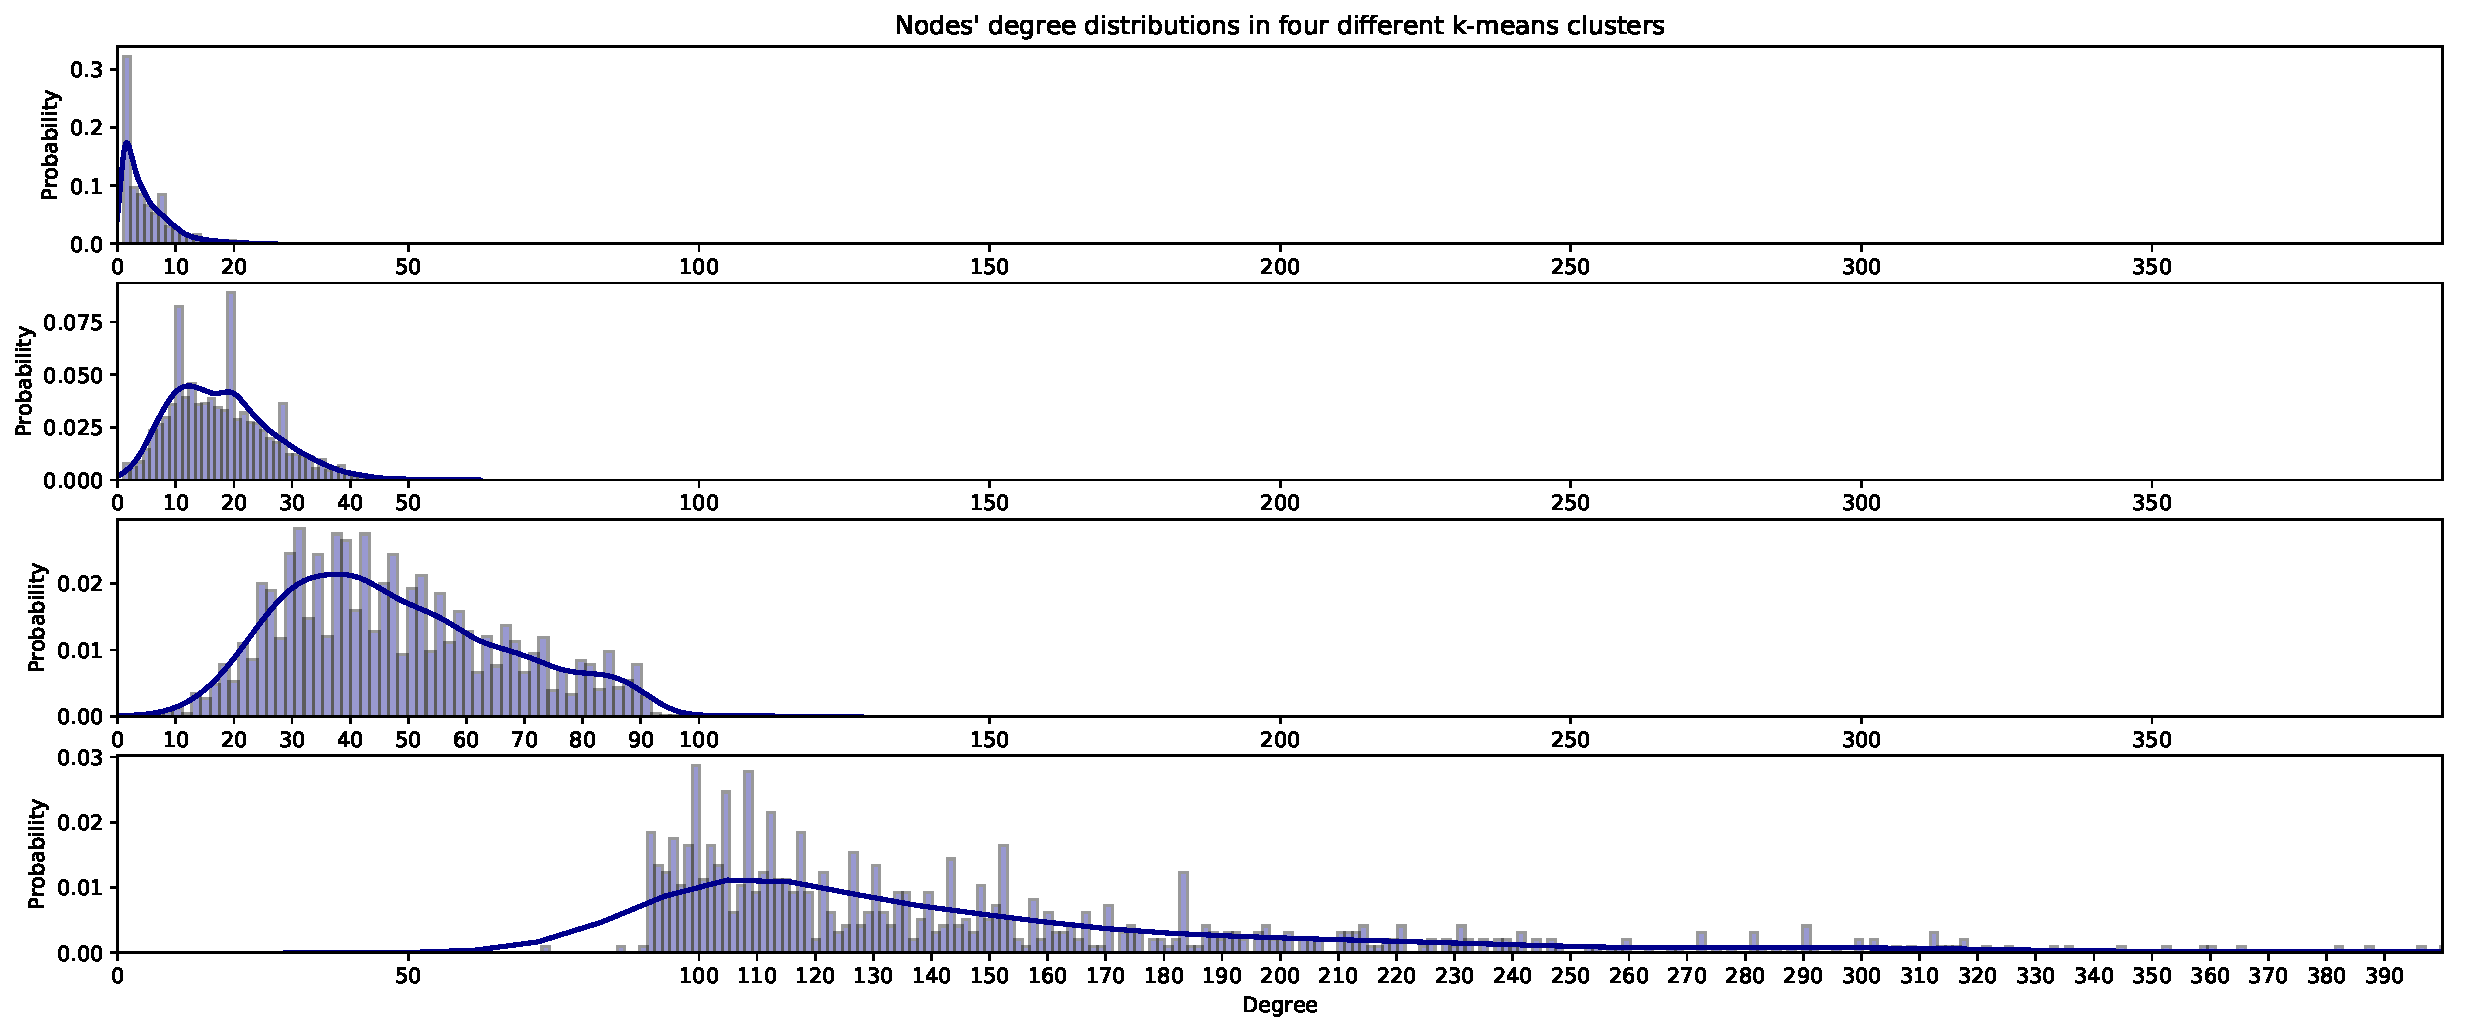
\includegraphics[width=1.0\textwidth]{images/evaluations/Fig44.pdf}\\
	\caption{Degree distribution of nodes in 4 k-means defined clusters. From the first to the fourth cluster top to bottom}
	\label{fig:Fig44}
\end{figure}

The first cluster is the most numerous since more than a third of the network's nodes have a small degree: ~36,2\% of nodes have degree lower than 10. However, this cluster is quite compact and adjoins with another cluster by one side. The reason for this lies in the local component affected the embeddings. The smooth transition from the first cluster to the second means that low-degree nodes usually communicate with the nodes of the second cluster, which have slightly higher degrees. The second cluster transits smoothly to the third. This observation highlights the network structure where nodes generally with small degrees tend to connect to nodes with slightly higher degrees and so on. In general, low-degree nodes are not directly connected to the network's hubs of the highest degrees. 

The fourth cluster of green colour on the~\autoref{fig:Fig43} consists of the nodes characterized by the highest degrees. This cluster is compact and well-separated from the rest of the network's nodes because of the particular degree classes allocation strategy. 12 degree classes were initially distinguished in the network. Nodes of the degrees from 1 to 90 were distributed over the first 11 classes while the rest nodes of the highest degrees from 90 to 1364 were assigned to the last class. The ordered sequences include hubs of different high degrees surrounded by the same degree class. This leads to the skip-gram model producing embeddings for hubs closer together because of the same degree class and pays less attention to the local component. That is why the low-dimensional representation places the cluster of hubs aside from other clusters. To confirm this reasoning, a more gradual degree classes split of 16 classes was tested on the~\autoref{fig:Fig46}. The smooth transition between clusters is clearly tracked here.

% \iffalse
\begin{figure}[!ht]
	\centering
	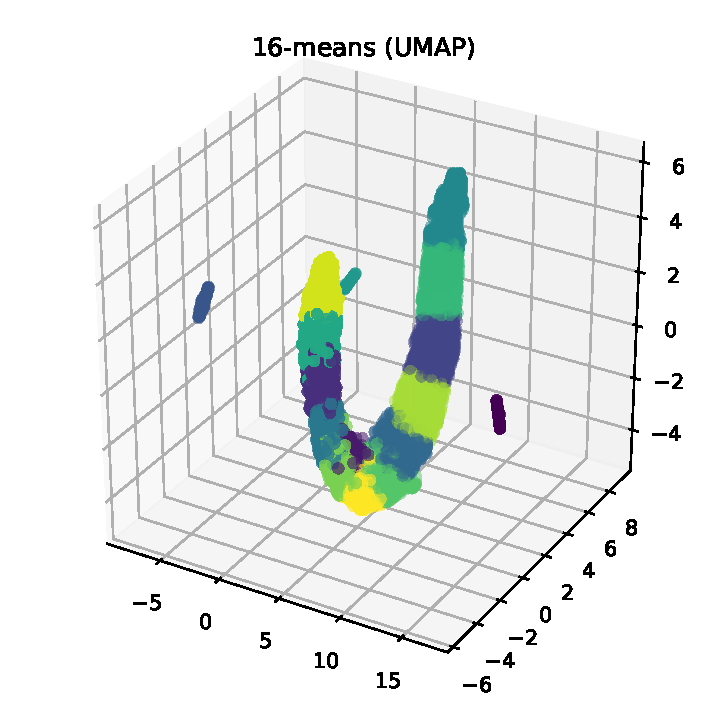
\includegraphics[width=0.4\textwidth]{images/evaluations/Fig46.pdf}\\
	\caption{Pipeline branch outcome visualization: local+global components -> UMAP -> $k$-means clustering (k=16).}
	\label{fig:Fig46}
\end{figure}
% \fi

The HDBSCAN outputs more coarse clusters than $k$-means under the all combinations of hyperparameters. The 27 combinations of hyperparameters min\_cluster\_size $\in$ [10,20,30], min\_samples $\in$ [5,20,40], and alpha $\in$ [0.25, 1.0, 1.3] leads to the same result of two separated clusters on the~\autoref{fig:Fig43} right. The nodes' degree distribution by clusters is on the~\autoref{fig:Fig44}. 
\begin{figure}[H]
	\centering
	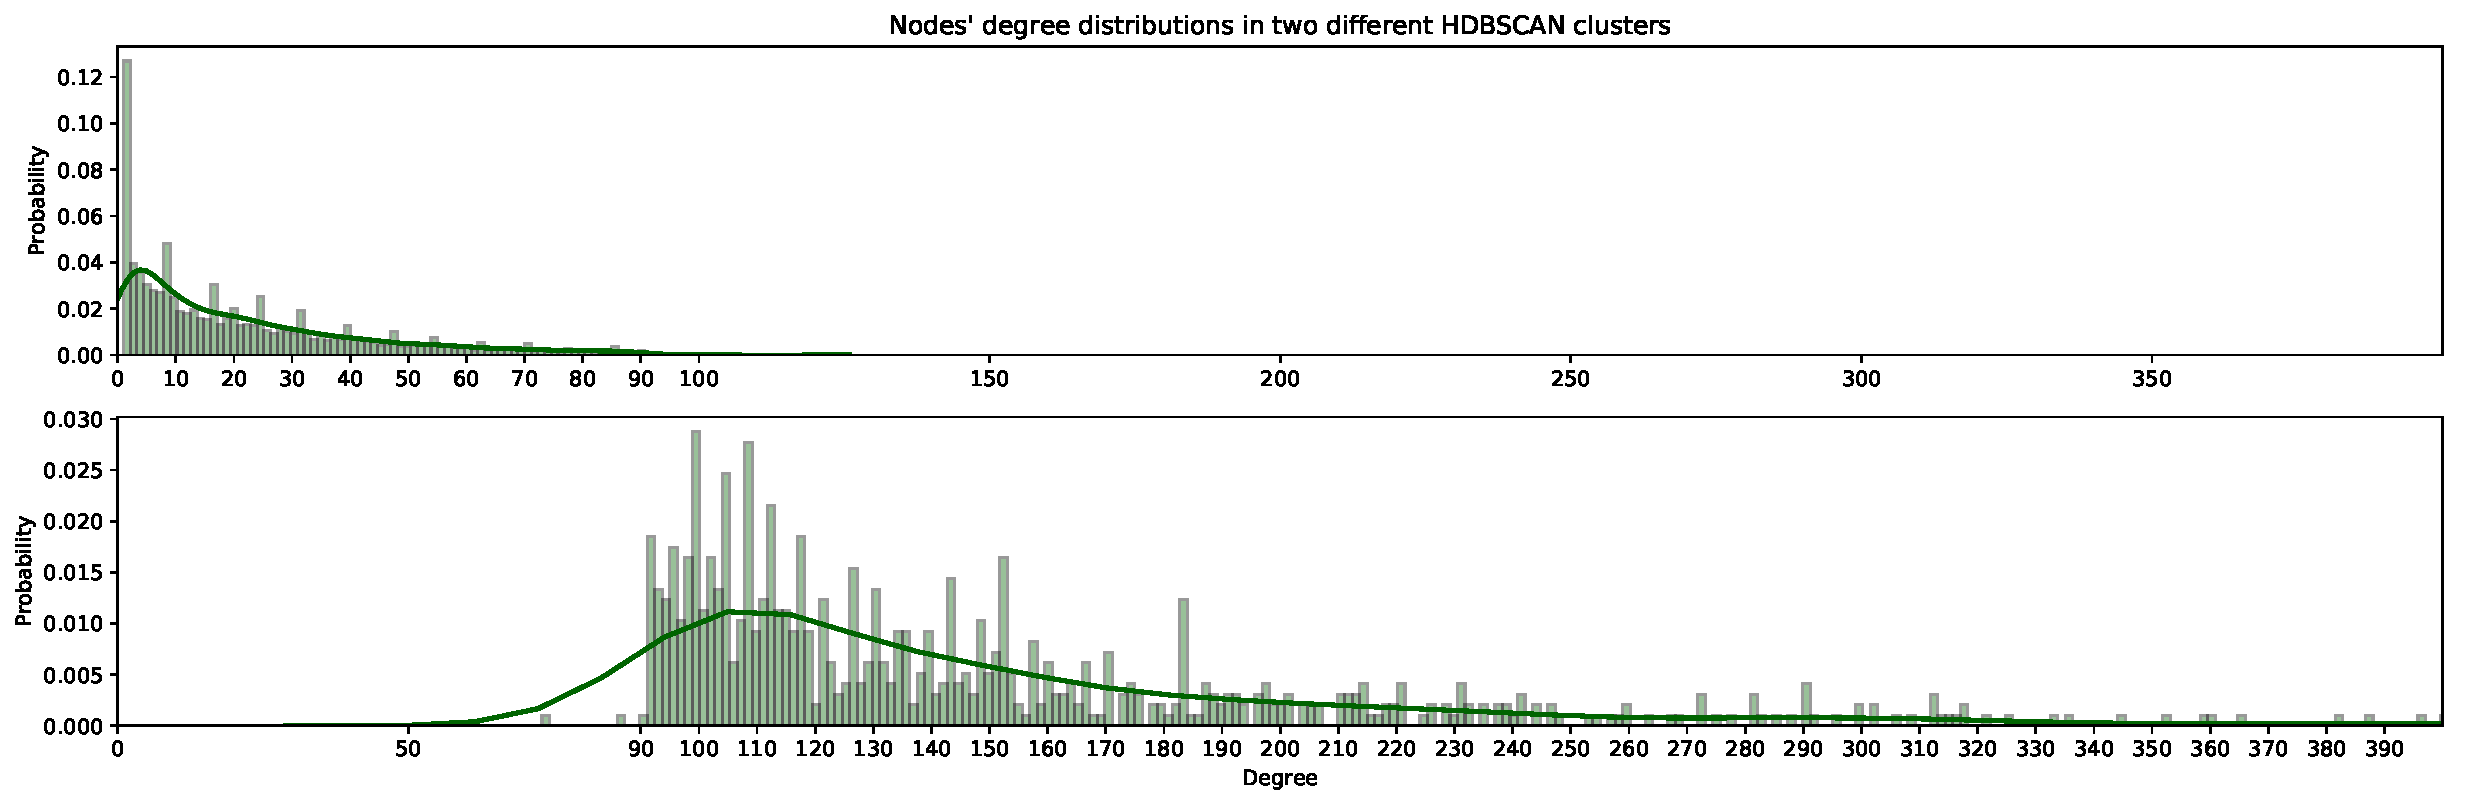
\includegraphics[width=1.0\textwidth]{images/evaluations/Fig45.pdf}\\
	\caption{Degree distribution of nodes in 2 HDBSCAN defined clusters. From the first to the second cluster top to bottom}
	\label{fig:Fig45}
\end{figure}
% \fi
    \begin{itemize}
        \item The first cluster consists of 11 126 nodes with the mean degree equal to 21.5. Its standard deviation is lower than the second cluster has - 20.9 (yellow data points on the right plot on the~\autoref{fig:Fig43}).
        \item the second cluster of HDBSCAN repeats the fourth cluster in $k$-means clustering: 754 nodes, mean of degrees equal to 165.9, standard deviation - 118.8 (violet data points on the right plot on the~\autoref{fig:Fig43})
    \end{itemize}
HDBSCAN finds dense non-globular clusters. The fact that the first cluster is relatively numerous evidences that nodes with degrees lower than 90 are well connected in the underlying network. Furthermore, these UMAP-reduced embeddings in the 3d metric space are dense enough to assign them to the same cluster. The rest separately allocated nodes serve as hubs in the network and belong to the second cluster.

The obtained experiment's result above demonstrated the analytical ability of UMAP approach to derive critical, meaningful information from the high-dimensional data better than others. The $k$-means clustering can capture the finer clusters due to the manual tuning of the hyperparameter $k$, whereas HDBSCAN relies mostly on the density of the points in a space and finds coarse-grained clusters unless clusters are separated with troughs of low density. Visualizations of the original financial network with nodes colored by $k$-means and HDBSCAN clustering labels can be found in the appendix 3.

\section{Summary}
This chapter presented the evaluation of the clustering results as the overall pipeline evaluation. The experiments on the real-world financial data set demonstrated the superiority of particular pipeline's branches over others for the particular input data set. The evaluation have been done by the set of internal clustering measures.

The result of the data science pipeline is strongly affected by the input data set and chosen hyperparameters. Therefore, this chapter suggested the ensemble of indices and heuristics for hyperparameters tuning as well as described the practical example of processing the real-world data set.

The chapter presented and compared the results from two pipeline's branches with the best outcomes according to the set of measures. The analysis of the other branches' results can be found in the appendices 1-2.

The next and last chapter of the current thesis will briefly revise the main points discussed in the work, summarize the main findings, provide some critical reviews, and point the direction for the future improvements.
\chapter{Conclusion}
\label{cha:conclusion}

The final chapter of this thesis includes the overview of the concept, discusses some critical aspects of the thesis, and concludes with potential future improvements and modifications.

\section{Overview of the thesis}

The overall goal of this thesis is to design and develop a concept and a data science pipeline for unsupervised node segmentation in financial transaction networks, that find groups of users similar in a structural and time sense.

Initially, the thesis discussed domain-specific features, which justify the motivation behind the problem statement. Some existing solutions for the same problem were presented along with their flaws and downsides. Thereupon, it moved to the overall goal, the possible contribution of the current work, and how developed approach can be applied to the real-world scenarios. The chapter~\ref{cha:background} presented existing approaches in machine learning domain which are extensively used by the concept. The special attention was paid to the network embedding learning approaches as it is in the core of the developed pipeline. The various research works on this topic explored static networks employing random walk models. Others emphasis the network structure's evolution over. There was only few research available on embedding features learning with existing network attributes incorporation. These works played an important role in this thesis, especially Node2ves~\cite{node2vec} and Role2vec~\cite{role2vec}. The former proposed breakthrough sampling strategy in networks and the latter developed a heuristic on nodes' structural similarity. Sections~\ref{Cluster Analysis} and~\ref{Dimensionality Reduction} covered the traditional and state-of-the-art unsupervised machine learning methods, their usage scenarios, functioning features, and limitations, which were highlighted by authors of competing methodologies. Thereby, the chapter~\ref{cha:background} aggregates insights from more than 50 external competent sources and provides a comprehensive summary of every presented technique. Such that it brings an understanding of the choice of the particular technique for the pipeline as well as a comprehension of their effect.

The concept and design chapter explained the proposed concept from a broader as well as a detailed perspective. It includes the conceptual illustration of the branched data science pipeline divided into main stages (\autoref{fig:Fig28}) along with the content of each stage. The main focus of the chapter is on the unique strategy sampling for network embeddings learning, which allows to incorporate available network attributes into Node2vec' semi-random walks. In the frame of this work, the time and degree attributes were selected. Potentially, one could select other attributes too. Additionally, the chapter covers the preparatory and final procedures as the data pre-processing and results' evaluation steps respectively. 

The following implementation chapter explained how the concept was implemented including the justifications of chosen technologies, used frameworks and tools. The data pre-processing step was mainly created taking the provided data set into consideration. Different data sets will require different adjustment of pre-processing techniques in order to produce meaningful result using the developed user segmentation pipeline. The automated feature learning framework described in section~\ref{Automated Feature Learning Framework} was implemented with the help of Node2vec 0.2.1 framework and several other common Python packages. The common machine learning techniques were implemented with the help of the recent existing frameworks listed in~\ref{Overall data science pipeline for user segmentation}. The common machine learning techniques were implemented with the help of the recent frameworks listed in~\ref{Overall data science pipeline for user segmentation}. All the pipeline's stages are bundled together in a Jupyter notebook named Pipeline. The notebook contains the results evaluation and interpretation sections with illustrations, comments, and explanations. Besides the notebook, another valuable outcome of the work is the web analytics application with some artificially generated data sets for the overall approach comprehension.

The last evaluation chapter presents various insights through plots and figures final segmentation outcomes as well as intermediate results. The outcomes are specific to the provided data set. The quality of a clustering result defined by the presence or absence of strong structural and/or time patterns hidden in the input network.

\section{Critical review}

There are some limitations of the current concept as well as its implementation, that came out of different reasons. Bellow some such aspects will be discussed 

\textbf{Application scenario.}
The data science pipeline has been tested on restricted real-world data set cut off in the number of observations. In general, this is not the best practice to manage the initial data, while all machine learning techniques only benefit from a large data set. To justify this decision, it has been done in order to facilitate the visualisation of observations in the cost of overall accuracy. 

\textbf{Data pre-processing.}
The data pre-processing step is firstly specific to input data and secondly user-defined. Although some intuitive heuristics on the time and degree classes split have been proposed, there is still uncertainty in this. Multiple runs of the pipeline with different splits on the same input data can help to develop some intuition in this regard and find a better split.

\textbf{Implementation.}
The pipeline is able to derive features from three possible combinations of time, local, and global structural components (loc + time, loc + glob, loc + time + glob). These three initial options are implemented in three different Jupyter notebooks. Probably, it would worth to come up with one file and implement this option via the input parameter of the pipeline. However, in this case, one file might become overwhelmed with the analytical illustrations and accompanying explanations for 18 branches results.

\textbf{Interpretation of the results.}
The obtained result strongly depends on the input data and user-defined parameters. To interpret the outcome, one should bear in mind the initial characteristics of the input data such as the time span, transaction distribution over time, degree distribution in the network and other related basic statistics. It can help a lot during the interpretation of the pipeline's result. Furthermore, some knowledge about the specific domain and data set origin are also of great help. In general, the interpretation task is very challenging and this work does not provide an unambiguous recipe either. Therefore the presented analysis is suitable for advanced network exploration additionally to the basic exploratory data analysis.

\section{Future work and research}

The developed approach is another try to learn a meaningful feature representation from dynamic networks, which could potentially explain the underlying network structure. This thesis presents a novel technique for sampling from a graph based on local structures of nodes' neighbourhoods, global structural graph attribute - degree, and time of transaction represented by edges of the graph. However, there is still a large scope for improvement and modification to the present developed approach.
\begin{itemize}
    \item \textbf{Consider directed graph. }In transaction data, users play different roles sending and receiving transactions. With high probability, in average the behavioural pattern for a sender will differ from the same for receiver's in terms of surrounding structures, the number of connections and operating time. A directed graph distinguish between senders and receivers. The preliminary analysis in this regard might help to interpret the pipeline's result and reveal new insights of user segmentation. Furthermore, the Node2vec framework can process directed networks. However, the proposed sampling strategy has to be revised.
    \item \textbf{Consider directed graph. }The obvious enhancement of processing a financial network is considering the amount of transferred assets. It is an edge-based attribute and is available in the standard Node2vec framework.
    \item \textbf{More intensive evaluation. }The current evaluation employs the set of internal clustering measures for globular and non-globular clusters. $k$-means clustering produces globular clusters and HDBSCAN produces clusters of arbitrary shapes. The overall results are compared by the reduced set of parameters which make sense for both techniques, although this set could be extended for better evaluation and comparison.
    \item \textbf{Finer hyperparameters tuning. }Although the pipeline provides semi-automated techniques on hyperparameters optimization, they can be improved and extended by the introduction of a finer scale and new optimizing techniques.
    \item \textbf{Experiments on another financial data set. }To confirm or deny the obtained conclusions, it would be beneficial to test the pipeline on another financial data set of different structure and origin.
\end{itemize}
To conclude, this thesis offers various insights about financial networks. Its users are nodes of the network and can be categorized based on their neighbourhoods in the network and graph-related attributes. The data science pipeline reveals the similarities between users according to their structural and time features within a network. This thesis explains how these similarities were obtained and how users were segmented under the minimum input information about participants. The thesis explains the concept, provides its implementation along with the web application to fully comprehend the idea.


%--------------------------------------------------------------
% TABLES, FIGURES, BIBLOGRAPHY AND APPENDICES
%--------------------------------------------------------------
\backmatter

% Lists of tables and figures
\listoftables
\listoffigures

% Bibliography
\setwidesite{}						% Set page to be wider for bibliography
\markboth{Bibliography}{bibliography}
\label{cha:bibliography}
\bibliographystyle{IEEEtran}
\bibliography{bibliography.bib}


% Use following to separate online (websites) and offline (books, papers) sources
%\printbibliography[heading=offline,filter=offline]
%\printbibliography[heading=online,filter=online]

\begin{appendices}
	\chapter{Appendix 1: Analysis of the network embedding learned from local structural and time components}
\label{appendix:k-means_time}

\section{$k$-means}
~\autoref{fig:App1} shows learned sets of embeddings reduced by three dimensionality reduction techniques.~\autoref{fig:App2} and~\autoref{fig:App3} provide visual insights into the optimal $k$ for $k$-means: PCA - $k$ = 3; t-SNE - $k$ = 3; UMAP - $k$ = 3.~\autoref{fig:App4} demonstrates the clustering results on data sets from ~\autoref{fig:App1}. The best clustering according to the set of internal clustering metrics is UMAP-reduced embeddings split into 3 clusters (right plot on~\autoref{fig:App4}).

\begin{figure}[!ht]
	\centering
	\includegraphics[width=1.0\textwidth]{images/appendix/App1.pdf}\\
	\caption{Embeddings sets reduced to 3 dimensions by three dimensionality reduction techniques.}
	\label{fig:App1}
\end{figure}
\begin{figure}[!ht]
	\centering
	\includegraphics[width=1.0\textwidth]{images/appendix/App2.pdf}\\
	\caption{Elbow plots for 3-dimensional embedding sets.}
	\label{fig:App2}
\end{figure}
\begin{figure}[!ht]
	\centering
	\includegraphics[width=1.0\textwidth]{images/appendix/App3.pdf}\\
	\caption{Evaluation of $k$-means clustering with respect to the number of clusters $k$.}
	\label{fig:App3}
\end{figure}
\begin{figure}[!ht]
	\centering
	\includegraphics[width=1.0\textwidth]{images/appendix/App4.pdf}\\
	\caption{Resulting $k$-means clustering.}
	\label{fig:App4}
\end{figure}

\section{HDBSCAN}

The sets from~\autoref{fig:App1} were clustered by HDBSCAN as well.~\autoref{fig:App9} suggests the best hyperparameters: PCA - min\_cluster\_size = 10, min\_samples = 5, alpha = 0.25;
t-SNE - min\_cluster\_size = 10, min\_samples = 5, alpha = 0.25; UMAP - min\_cluster\_size = 10, min\_samples = 40, alpha = 0.25.~\autoref{fig:App10} shows the coloured by defined HDBSCAN clusters embeddings. The best clustering according to the set of internal clustering metrics is t-SNE-reduced embeddings split into 2 clusters (middle plot on~\autoref{fig:App10}).

\begin{figure}[!ht]
	\centering
	\includegraphics[width=1.0\textwidth]{images/appendix/App9.pdf}\\
	\caption{Evaluation of HDBSCAN clustering with respect to the set of hyperparameters.}
	\label{fig:App9}
\end{figure}
\begin{figure}[!ht]
	\centering
	\includegraphics[width=1.0\textwidth]{images/appendix/App10.pdf}\\
	\caption{Resulting HDBSCAN clustering.}
	\label{fig:App10}
\end{figure}

\section{Interpretation of the results}
Some initial time analysis is needed to get an idea about overall time distribution in the network. The continuous period of explored part of the network spans approximately 13 months so that 26 consecutive time classes were allocated each of length of ~15 days. It is turned out that some of the users were active during several time classes, whereas the majority belong to only one class.~\autoref{fig:App13} shows the number of nodes by the number of time classes when they were active. Out of more than 11k nodes, almost 5k belong to more than one time classes.

\begin{figure}[!ht]
	\centering
	\includegraphics[width=1.0\textwidth]{images/appendix/App13.pdf}\\
	\caption{Number of nodes in the network by the number of time classes.}
	\label{fig:App13}
\end{figure}

A node, which was active in several time classes, is assigned to the class when it sent and received most transfers.~\autoref{fig:App14} describes how many nodes were the most active in every time class.

\begin{figure}[!ht]
	\centering
	\includegraphics[width=1.0\textwidth]{images/appendix/App14.pdf}\\
	\caption{Count of the most active nodes per time class.}
	\label{fig:App14}
\end{figure}

~\autoref{fig:App15} provides a close look at the clusters produces by k-means. The numbers of nodes in each cluster are 3362, 3591, and  4926 from top to bottom respectively. From the figure it can be seen that the first cluster slightly overlaps with the second in terms of when users of each cluster were active. The first cluster consists of users mostly active by the end of the period. The users of the second cluster were the most active earlier in time and almost stop operating later on.  The third cluster unites nodes active over the entire period. The first six periods are naturally almost empty for all clusters because of the overall nodes distribution by time classes on~\autoref{fig:App14}.

\begin{figure}[!ht]
	\centering
	\includegraphics[width=1.0\textwidth]{images/appendix/App15.pdf}\\
	\caption{Time classes distribution of nodes in 3 $k$-means defined clusters in UMAP-redused set. From the first to the third cluster top to bottom.}
	\label{fig:App15}
\end{figure}

HDBSCAN clusters of the t-SNE reduced set of embeddings look interesting. The distribution of time classes within 2 clusters (137 and 11741 nodes) is depicted on~\autoref{fig:App16}. It is notable that some group of users have been operating within each other over time classes $l-m$ as they are connected also by local structural component.

\begin{figure}[!ht]
	\centering
	\includegraphics[width=1.0\textwidth]{images/appendix/App16.pdf}\\
	\caption{Time classes distribution of nodes in 2 HDBSCAN defined clusters in t-SNE-redused set. From the first to the second cluster top to bottom.}
	\label{fig:App16}
\end{figure}

	\chapter{Appendix 2: Analysis of the network embedding learned from local structural, global structural, and time components}
\label{appendix:k-means_time_struc}

\section{$k$-means}
~\autoref{fig:App5} shows learned sets of embeddings reduced by three dimensionality reduction techniques.~\autoref{fig:App6} and~\autoref{fig:App7} provide visual insights into the optimal $k$ for $k$-means: PCA - $k$ = 4; t-SNE - $k$ = 4; UMAP - $k$ = 5.~\autoref{fig:App8} demonstrates the clustering results on data sets from ~\autoref{fig:App6}. The best clustering according to the set of internal clustering metrics is UMAP-reduced embeddings split into 5 clusters (right plot on~\autoref{fig:App5}).

\begin{figure}[!ht]
	\centering
	\includegraphics[width=1.0\textwidth]{images/appendix/App5.pdf}\\
	\caption{Embedding set reduced to 3 dimensions by three dimensionality reduction techniques.}
	\label{fig:App5}
\end{figure}
\begin{figure}[!ht]
	\centering
	\includegraphics[width=1.0\textwidth]{images/appendix/App6.pdf}\\
	\caption{Elbow plots for 3-dimensional embedding sets.}
	\label{fig:App6}
\end{figure}
\begin{figure}[!ht]
	\centering
	\includegraphics[width=1.0\textwidth]{images/appendix/App7.pdf}\\
	\caption{Evaluation of $k$-means clustering with respect to the number of clusters $k$.}
	\label{fig:App7}
\end{figure}
\begin{figure}[!ht]
	\centering
	\includegraphics[width=1.0\textwidth]{images/appendix/App8.pdf}\\
	\caption{Resulting $k$-means clustering.}
	\label{fig:App8}
\end{figure}

\section{HDBSCAN}
The sets from~\autoref{fig:App5} were clustered by HDBSCAN as well.~\autoref{fig:App11} suggests the best hyperparameters: PCA - min\_cluster\_size = 20, min\_samples = 5, alpha = 0.25;
t-SNE - min\_cluster\_size = 30, min\_samples = 40, alpha = 0.25; UMAP - min\_cluster\_size = 10, min\_samples = 20, alpha = 0.25.~\autoref{fig:App12} shows the coloured by defined HDBSCAN clusters embeddings. The best clustering according to the set of internal clustering metrics is PCA-reduced embeddings split into 2 clusters (left plot on~\autoref{fig:App12}).

\begin{figure}[!ht]
	\centering
	\includegraphics[width=1.0\textwidth]{images/appendix/App11.pdf}\\
	\caption{Evaluation of HDBSCAN clustering with respect to the set of hyperparameters.}
	\label{fig:App11}
\end{figure}
\begin{figure}[!ht]
	\centering
	\includegraphics[width=1.0\textwidth]{images/appendix/App12.pdf}\\
	\caption{Resulting HDBSCAN clustering.}
	\label{fig:App12}
\end{figure}

\section{Interpretation of the results}
Some initial time analysis was done in appendix 1 (~\autoref{fig:App13} and ~\autoref{fig:App14}). The degree distribution of the initial network is on the~\autoref{fig:App17}. It follows Power law distribution: the majority of nodes have low degrees and minority - high degrees.

~\autoref{fig:App18} shows degree distribution and distribution of nodes by time classes within each of 5 $k$-means clusters of the UMAP-redused set of embeddings. Characteristics of the clusters on the~\autoref{fig:App19} by their degree and time classes distributions on the ~\autoref{fig:App18} (top to bottom):
    \begin{enumerate}
        \item 1902 nodes (violet) - mean 62.4 - std 61.6
        \item 1949 nodes (blue) - mean 46 - std 64.7
        \item 2163 nodes (light green) - mean 12.5 - std 8.4
        \item 2284 nodes (yellow) - mean 49 - std 60.7
        \item 3579 nodes (dark green) - mean 4.8 - std 4.5
    \end{enumerate}
The majority of the nodes with low degrees from all possible time classes are accumulated in the most numerous fifth cluster. The fifth dark green cluster penetrates to the third light green cluster, whose average degree is slightly higher and nodes mostly act in the latest periods. It might be assumed that nodes on the periphery of the network do not tend to connect to hubs of high degree directly, but by paths through nodes of steadily increasing degrees. The degree distribution within the first class is right-skewed with heavy right tail, where the most hubs are. This cluster is not adjacent to the fifth, and this fact supports the above hypothesis about network structure.

Another observation is the second blue cluster consists of nodes being active in the earlier periods. It does not connect to the first violet and the third light green clusters, whose nodes were active mostly in recent periods. The second blue and the fourth yellow clusters adjoin and have a long border, which was hard to spot by the structure of the set. Their degree and time classes distributions are quite similar. 

The closer look at the second blue -> fourth yellow -> first violet clusters in exactly this sequence reveal some insights: 
\begin{itemize}
    \item degree distributions are right-skewed and their means move gradually to the right from blue cluster to the violet over the set.
    \item the time classes distributions within these three clusters are characterised as the earliest active nodes -> active nodes in the middle time period -> active nodes in the recent time periods. This is also reflected in the gradual transition from the blue -> yellow -> violet clusters.
\end{itemize}

The assumptions made above were based mostly on the clusters adjacency in the representation space. The transitions between clusters help to understand what kinds of nodes of the network tend to communicate with each other.
\begin{figure}[!ht]
	\centering
	\includegraphics[width=1.0\textwidth]{images/appendix/App17.pdf}\\
	\caption{Degree distribution of the financial network.}
	\label{fig:App17}
\end{figure}
\begin{figure}[!ht]
	\centering
	\includegraphics[width=0.4\textwidth]{images/appendix/App19.pdf}\\
	\caption{$k$-means ($k$=5) clustering on UMAP-reduced set of embeddings.}
	\label{fig:App19}
\end{figure}
\begin{figure}[!ht]
	\centering
	\includegraphics[width=0.9\textwidth]{images/appendix/App18.pdf}\\
	\caption{Degree and time classes distributions of nodes within each of 5 $k$-means clusters of the UMAP-redused set of embeddings.From the first to the fifth cluster top to bottom.}
	\label{fig:App18}
\end{figure}

The HDBSCAN clustering on the PCA reduced set (the best out of others according to the ensemble of internal clustering metrics), in this case, produced a poor result. ~5.5\% nodes were recognized as noise - grey colour on~\autoref{fig:App20}, ~0.4\% nodes make up two clusters, and 94\% is in the last cluster. The degree and time classes distributions of the last cluster is on the~\autoref{fig:App21} bottom.

\begin{figure}[!ht]
	\centering
	\includegraphics[width=0.4\textwidth]{images/appendix/App20.pdf}\\
	\caption{HDBSCAN clustering on PCA-reduced set of embeddings.}
	\label{fig:App20}
\end{figure}
\begin{figure}[!ht]
	\centering
	\includegraphics[width=0.9\textwidth]{images/appendix/App21.pdf}\\
	\caption{Degree and time classes distributions of nodes within the HDBSCAN clusters of the PCA-redused set of embeddings. From the first to the fourth cluster top to bottom.}
	\label{fig:App21}
\end{figure}
	\chapter{Appendix 3: Visualization of the financial network}
\label{appendix:k-means_time_struc}

\iffalse
\begin{figure}[!ht]
	\centering
	\includegraphics[width=1.0\textwidth]{images/appendix/k-means_white.pdf}\\
	\caption{Financial network of Prosper.com users. Node size denotes degree; Node colour denotes $k$-means clustering labels of 4 clusters (pipeline branch: loc+glob -> UMAP -> $k$-means)}
	\label{fig:App20}
\end{figure}

\begin{figure}[!ht]
	\centering
	\includegraphics[width=1.0\textwidth]{images/appendix/hdbscan_white.pd}\\
	\caption{Financial network of Prosper.com users. Node size denotes degree; Node colour denotes HDBSCAN clustering labels of 2 clusters (pipeline branch: loc+glob -> UMAP -> HDBSCAN)}
	\label{fig:App21}
\end{figure}

\fi
\end{appendices}

\end{document}
